\section{Breve historia de la teoría de la difracción: de las sombras al mundo vectorial}

	Durante más de dos mil años, desde Euclides hasta el umbral del Renacimiento, la óptica geométrica descansó sobre un único supuesto, casi evidente por sí mismo: la luz viaja en línea recta \cite{herzberger1966optics}. Un rayo recto proyecta una sombra de borde recto, y todo niño que alguna vez ha jugado con su propia silueta sobre una pared lo ha confirmado mil veces. Esta imagen explicaba tan bien los espejos, las lentes y los eclipses que, durante siglos, a nadie se le ocurrió mirar de cerca el borde mismo de una sombra para preguntarse qué ocurre realmente en esa delgada franja fronteriza donde la luz se detiene y comienza la oscuridad. La difracción es la historia de lo que se ocultaba en esa frontera, y de cómo un solo detalle pasado por alto, perseguido pacientemente durante tres siglos, obligó a los físicos a reconstruir por completo su comprensión de lo que es la luz. Es, en un sentido muy real, la historia de la luz negándose a ser simplificada.

	El primero en mirar con suficiente cuidado fue un jesuita italiano llamado Francesco Maria Grimaldi. Hacia 1660, trabajando en una habitación oscurecida en Bolonia, Grimaldi dejó pasar un haz estrecho de luz solar a través de una pequeña abertura y lo hizo cruzar el borde de una varilla antes de incidir sobre una pantalla. La geometría ordinaria hacía una predicción firme: una sombra de borde nítido, oscura de un lado y clara del otro, sin nada más que decir. Lo que Grimaldi vio en cambio era más extraño y mucho más delicado: el límite de la sombra no era una línea limpia sino un flequillo suave, entretejido con tenues bandas de color, y la sombra misma era ligeramente más ancha de lo que la geometría pura permitía. La luz estaba, de alguna manera, alcanzando el espacio al que no debía llegar, y curvándose de maneras en que ningún rayo podría curvarse. Grimaldi no vivió para ver su trabajo impreso; sus observaciones aparecieron solo después de su muerte, en el libro de 1665 \textit{Physico-Mathesis de Lumine} \cite{grimaldi1665physico}. Allí bautizó el efecto con el nombre de \textit{diffractio}, del latín para «romperse en pedazos», porque a él le parecía como si la luz misma se hubiera hecho añicos en el borde del obstáculo. Fue una observación notablemente premonitoria, hecha con nada más que luz solar, una habitación oscura y un ojo agudo, y durante mucho tiempo casi nadie notó que se había hecho.

	La razón por la que casi nadie lo notó tiene, en buena parte, un nombre propio: Isaac Newton. El propio Newton había visto delicados anillos de colores formarse entre una lente y una placa de vidrio plana —el patrón que hoy seguimos llamando los anillos de Newton— y los describió meticulosamente en su propia \textit{Opticks} de 1704 \cite{newton1704opticks}. Sin embargo, Newton seguía convencido de que la luz estaba hecha de pequeñas partículas, corpúsculos, disparados en línea recta, y encajó esos desconcertantes colores en esa imagen lo mejor que pudo en lugar de dejar que la hicieran tambalear. La autoridad científica de Newton en el siglo XVIII era tan enorme que discrepar de él era casi un suicidio profesional, de modo que las franjas de Grimaldi, y el razonamiento ondulatorio que podría haberlas explicado, quedaron silenciosamente arrinconadas durante más de cien años. Es una de las grandes advertencias de la física: la evidencia de la difracción estuvo a la vista todo ese tiempo, esperando a alguien dispuesto a tomarla en serio.

	Alguien lo hizo, aunque su idea llegó un poco adelantada a su tiempo y sin la maquinaria suficiente para terminar el trabajo. En 1690 el físico holandés Christiaan Huygens propuso, en su \textit{Traité de la Lumière} \cite{huygens1690traite}, una manera casi juguetona de imaginar cómo avanza una onda. Imaginemos, decía Huygens, que cada punto de un frente de onda es en sí mismo una pequeña fuente, que emite su propia ondita circular. Un instante después, el nuevo frente de onda es simplemente la envolvente suave que rodea a todas esas innumerables onditas a la vez. Esta imagen, conocida hoy como el principio de Huygens, explicaba maravillosamente la reflexión y la refracción, y sugería que una onda podía, en efecto, colarse lateralmente hacia una sombra geométrica, ya que las onditas que se propagan desde puntos cercanos al borde de un obstáculo no tienen a dónde ir salvo hacia ese espacio prohibido. Lo que la construcción de Huygens todavía no podía explicar era por qué las franjas claras y oscuras resultantes aparecían exactamente donde aparecían, porque él no tenía noción de que las pequeñas onditas pudieran reforzarse en algunos lugares y cancelarse en otros. Esa idea faltante era la interferencia, y suministrarla tomaría más de un siglo.

	Finalmente llegó en unos pocos años notables al comienzo del siglo XIX. En 1801, el polímata inglés Thomas Young realizó el experimento que todo estudiante de óptica encuentra tarde o temprano: dejó pasar la luz por dos rendijas estrechas y muy próximas entre sí, y observó el patrón que formaba sobre una pantalla más allá \cite{young1804bakerian}. En lugar de dos bandas brillantes, vio muchas —toda una secuencia de franjas claras y oscuras, exactamente como cabría esperar si dos onditas superpuestas en un estanque pudieran a veces coronarse juntas y a veces cancelarse hasta la quietud. La luz, concluyó Young, debe ser una onda, y las ondas pueden sumarse o restarse. Fue un experimento devastadoramente simple que llevaba una conclusión enorme, y precisamente por eso fue recibido en Inglaterra con desdén más que con aplausos; atacar a Newton todavía no era un deporte popular. La reivindicación llegó desde Francia. Entre 1815 y 1820 el joven ingeniero Augustin-Jean Fresnel tomó las onditas de Huygens y la interferencia de Young y las soldó en un único principio cuantitativo —el principio de Huygens-Fresnel— capaz de predecir, por primera vez, exactamente cuán brillante u oscuro debía ser cualquier punto de un patrón de difracción \cite{fresnel1819memoire}. Fresnel no se limitó a describir la difracción cualitativamente, como habían hecho Grimaldi y Huygens; la calculó, tratando cada punto de una abertura como una fuente genuina de ondas secundarias cuyas onditas debían sumarse, cresta contra cresta y valle contra valle, para hallar la luz en cualquier punto más allá.

	La teoría de Fresnel entregó entonces uno de los momentos más célebres de la historia de la física. La Academia Francesa de las Ciencias, todavía en buena parte incrédula, propuso la difracción como tema de un concurso con premio, y el matemático Siméon Denis Poisson, escéptico confeso de la imagen ondulatoria, examinó las ecuaciones de Fresnel buscando un absurdo que las hundiera de una vez por todas. Encontró lo que buscaba, o creyó encontrarlo: las propias matemáticas de Fresnel predecían que, justo en el centro de la sombra proyectada por un pequeño disco circular, directamente detrás del obstáculo donde el sentido común garantiza oscuridad total, debía haber un punto brillante de luz. Poisson presentó esto como una reducción al absurdo, confiado en que jamás podría observarse tal cosa. El presidente de la academia, Dominique Arago, decidió realmente llevar a cabo el experimento en lugar de discutir sobre él, y allí, brillando tenuemente en el corazón de la sombra del disco, estaba el punto que Poisson había predicho en son de burla. El punto de Poisson-Arago, como se le conoce hoy con cierta ironía, se convirtió en una de las confirmaciones experimentales más espectaculares que teoría alguna haya recibido jamás, y zanjó el pleito entre partículas y ondas por el resto del siglo.

	El éxito de Fresnel, sin embargo, se apoyaba en una intuición inspirada más que en una derivación rigurosa: su integral funcionaba extraordinariamente bien, pero nadie había demostrado que se siguiera necesariamente de la propia ecuación de onda. Esa brecha fue cerrada en 1883 por el físico alemán Gustav Kirchhoff, quien empleó las matemáticas del teorema de Green para derivar la integral de difracción de Fresnel directamente a partir de la ecuación de onda, colocando toda la construcción sobre un cimiento matemático firme \cite{kirchhoff1883theorie}. La formulación de Kirchhoff se convirtió, y en gran medida sigue siendo, el caballo de batalla de lo que hoy llamamos la teoría escalar de la difracción: trata la luz como una única ondulación escalar en vez de como el vector electromagnético completo, una aproximación que funciona notablemente bien siempre que los obstáculos involucrados sean mucho mayores que la longitud de onda de la luz. Hubo, es cierto, una sutil grieta lógica en el argumento de Kirchhoff —sus condiciones de frontera exigían que tanto el campo como su derivada se anularan simultáneamente detrás de una pantalla opaca, un requisito matemáticamente excesivo— y fue Henri Poincaré quien primero lo señaló. La grieta fue subsanada en 1896 por Arnold Sommerfeld, quien halló una solución alternativa, plenamente autoconsistente, para la difracción por un borde recto y un semiplano, eliminando la inconsistencia sin sacrificar nada del éxito práctico de Kirchhoff \cite{sommerfeld1896mathematische, sommerfeld1954optics}.

	Todo esto, por ingenioso que fuera, seguía tratando la luz como un único número que oscila en lugar de la cantidad vectorial que, según las ecuaciones de Maxwell, verdaderamente es —y a comienzos del siglo XX esa omisión empezó a importar. En 1908 Gustav Mie resolvió exactamente las ecuaciones de Maxwell para la dispersión de la luz por una pequeña esfera, conservando todo el contenido vectorial y de polarización del campo \cite{mie1908beitrage}; su resultado explica, entre muchas otras cosas, por qué el cielo es azul y por qué las nubes y la leche son blancas, y sigue siendo indispensable siempre que la luz interactúa con partículas de tamaño comparable al de su propia longitud de onda. Al año siguiente Peter Debye extendió el mismo pensamiento vectorial al foco estrecho de una lente, mostrando que cerca de un punto focal agudo la aproximación escalar simplemente se derrumba. La síntesis de todo lo anterior —la integral de Fresnel, el rigor de Kirchhoff y Sommerfeld, y las correcciones vectoriales completas de Mie y Debye— quedó finalmente reunida en una única referencia monumental por Max Born y Emil Wolf, cuyo \textit{Principles of Optics} (1959) ha servido desde entonces como la biblia del campo \cite{born1999principles}. Born y Wolf dejaron explícito exactamente cuándo es confiable la imagen escalar más simple y cuándo falla del todo: en lentes de alta apertura numérica, en materiales anisótropos o quirales, y siempre que las estructuras relevantes se reducen a la escala de la propia longitud de onda, la naturaleza vectorial de la luz ya no puede ignorarse.

	La invención del láser en 1960 le dio a la teoría de la difracción una urgencia práctica enteramente nueva, ya que de pronto proporcionó una fuente de luz suficientemente coherente y controlable como para explotar la difracción a propósito en lugar de simplemente tolerarla. \textit{Introduction to Fourier Optics} (1968), de Joseph Goodman, replanteó todo el tema de una manera hermosamente económica: un sistema óptico, mostró Goodman, puede tratarse como una especie de procesador de señales, y el patrón de difracción producido lejos de una abertura es, para todos los efectos prácticos, el mismo objeto matemático que la transformada de Fourier de la forma de esa abertura \cite{goodman2005introduction}. Este único replanteamiento abrió la puerta a la holografía, a lentes difractivas que enfocan la luz mediante patrones grabados en vez de vidrio curvo, y a la corrección computacional de aberraciones en cámaras y telescopios modernos.

	La historia todavía se está escribiendo. Hoy, los ingenieros graban \textit{metasuperficies} —arreglos de estructuras a escala nanométrica, mucho más pequeñas que la longitud de onda de la luz— que remodelan la fase y la polarización de un frente de onda punto por punto, permitiendo que una lámina apenas más gruesa que un cabello humano haga el trabajo de toda una pila de lentes \cite{yu2011light}. La difracción de electrones y de rayos X, gobernada exactamente por la misma lógica ondulatoria que Fresnel y Kirchhoff dedujeron para la luz visible, permite a los científicos cartografiar la arquitectura atómica de cristales y moléculas —fue, después de todo, la difracción de rayos X la que reveló por primera vez la estructura de doble hélice del ADN. Y la difracción impone un límite absoluto e infranqueable a lo que cualquier instrumento óptico puede llegar a resolver: ningún telescopio, por perfectamente pulido que esté, y ningún microscopio, por costosamente construido que sea, puede enfocar la luz hasta un punto matemático, porque el mismo acto de hacer pasar la luz por una abertura finita vuelve a esparcirla. Toda imagen que un telescopio o un microscopio hayan producido jamás, desde las primeras lunas borrosas que Galileo esbozó hasta las fotografías más nítidas que los observatorios más grandes pueden ofrecer hoy, lleva estampada sobre la luz misma la firma de la difracción. Tres siglos y medio después de que un jesuita notara que una sombra en una habitación oscura de Bolonia no era tan nítida como exigía la geometría, la difracción ha crecido desde una curiosa imperfección hasta convertirse en una de las ideas más profundas y útiles de toda la física —y, como los capítulos que siguen mostrarán con cuidado en detalle, todavía tiene mucho que enseñarnos sobre la naturaleza de la luz.

\section{Teoría escalar de la difracción}\label{Sec:Diffraction}

	Como es bien sabido a partir de las ecuaciones de onda eléctrica y magnética con fuentes, las ondas electromagnéticas son muy ricas en su naturaleza y en la naturaleza que pueden crear como ondas. En este capítulo vamos a estudiar este comportamiento ondulatorio de la luz; sin embargo, al tratarse de unas notas introductorias, resolver esas dos ecuaciones resulta difícil, y si pretendiéramos resolverlas analíticamente, eso sería completamente imposible.

	Para hacer física es muy frecuente imponer supuestos sobre el modelo con el fin de hacerlo más fácil de entender y desarrollar, o incluso, de calcular soluciones analíticas. En este capítulo vamos a contar cuántos supuestos necesitamos para llegar a la teoría escalar de la difracción. Teniendo esto en cuenta, comencemos con el primero.

	\begin{Assumption}
		En la propagación de la luz la interacción magnética es completamente nula.
	\end{Assumption}

	Esto debe hacerse porque, en la naturaleza, las interacciones magnéticas son más ricas que las eléctricas; sin embargo, por curioso que suene, esto hace que las soluciones de la ecuación de onda magnética con fuentes sean mucho más difíciles de calcular. Por lo tanto, la formulación electromagnética puede entenderse únicamente por medio de la ecuación de onda eléctrica
	\begin{equation*}
		\left(\nabla^2 - \frac{1}{C}^2 \frac{\partial^2}{\partial t^2}\right)\vec{E} = \frac{1}{\epsilon_0}\bm{\nabla}\rho + \mu_o \frac{\partial}{\partial t}\vec{J}.
	\end{equation*}
	Sin embargo, esta ecuación de onda es realmente difícil de resolver de manera exacta, y la mayoría de las soluciones se encontrarán de forma numérica. Así que, para simplificarnos la vida, vamos a usar el siguiente supuesto

	\begin{Assumption}
		La onda eléctrica se propaga en el vacío, no existen densidades de carga ni densidades de corriente.
	\end{Assumption}
	Bajo estos supuestos, la ecuación de onda adopta la conocida forma
	\begin{equation}
		\nabla^2 \vec{E} = \frac{1}{C^2}\frac{\partial^2}{\partial t^2}\vec{E}
	\end{equation}

	Al estudiar el comportamiento vectorial de la radiación electromagnética se llega al concepto de polarización, que describe el comportamiento vectorial de la luz, y se encuentra que, en general, este comportamiento vectorial está confinado a una elipse, conocida como la elipse de polarización. Así, en general, el vector eléctrico está dado por
	\begin{equation}
	\vec{E}(\vec{r},t) = E(\vec{r},t) \, \hat{\vec{e}}(\vec{r},t),
	\end{equation}
	donde $E(\vec{r},t)$ denota la amplitud del campo y $\hat{\vec{e}}(\vec{r},t)$ representa el vector de polarización, el cual, además de variar en el espacio, puede evolucionar en el tiempo de manera estocástica.

	La ecuación de onda asociada toma entonces la forma
	\begin{equation}
	\nabla^2 \left[ E(\vec{r},t)\hat{\vec{e}}(\vec{r},t) \right] - \mu\varepsilon \frac{\partial^2}{\partial t^2} \left[ E(\vec{r},t)\hat{\vec{e}}(\vec{r},t) \right] = 0,
	\end{equation}
	cuya solución directa presenta complejidades notables. Para abordar este problema se recurre a estrategias de simplificación, como descomponer el campo en componentes escalares. Estas soluciones escalares pueden combinarse después para reconstruir el comportamiento vectorial completo.

	La variación temporal de la amplitud, la fase y la polarización se analiza rigurosamente mediante la teoría de la coherencia (explorada en profundidad en el Capítulo~\ref{chap:Coherencia}). No obstante, bajo ciertas aproximaciones la dependencia temporal de la amplitud se atribuye únicamente a las oscilaciones intrínsecas del campo, mientras que la polarización se considera estática. Además, desde un punto de vista electromagnético, el estado de polarización está completamente determinado por los coeficientes de Fresnel, por lo que en cada posición espacial la onda eléctrica puede tener un estado de polarización completamente distinto, así que vamos a necesitar hacer algunos supuestos adicionales:

	\begin{Assumption}
		La polarización de la onda no evoluciona en el tiempo.
	\end{Assumption}
	\begin{Assumption}
		La polarización de la onda no cambia en ningún punto del espacio, siendo completamente isótropa y homogénea en el espacio.
	\end{Assumption}

	Bajo estos dos supuestos, el campo eléctrico se simplifica a
	\begin{equation}
	\vec{E}(\vec{r},t) = E(\vec{r},t) \, \hat{\vec{e}}(\vec{r}),
	\end{equation}
	lo que permite su expansión en una base de polarización ortogonal,
	\begin{equation}
	\vec{E}(\vec{r},t) = E_1(\vec{r},t)\hat{\vec{e}}_1 + E_2(\vec{r},t)\hat{\vec{e}}_2.
	\end{equation}

	Sin embargo, permitir esta expresión conlleva otro supuesto. Como se ha visto al estudiar la polarización, se trata de una aproximación que permite estudiar el campo eléctrico pasando de una perspectiva $3D$ a una $2D$; esto se debe a que el campo eléctrico y el magnético, bajo nuestras condiciones, son ortogonales a la dirección de propagación, y el frente de onda es suave. Resumiendo, el supuesto empleado para expresar la polarización como la superposición de dos estados ortogonales $\left\{\hat{e}_1, \hat{e}_2 \right\}$ es

	\begin{Assumption}
		Los campos eléctrico y magnético que componen la onda electromagnética son ortogonales al eje de propagación, de modo que el comportamiento vectorial está dado por $2$ vectores de polarización.
	\end{Assumption}

	Cada componente escalar $E_i$ satisface individualmente la ecuación de onda
	\begin{equation}
	\nabla^2 E_i - \mu\varepsilon \frac{\partial^2 E_i}{\partial t^2} = 0 \quad (i=1,2),
	\end{equation}
	desacoplando así el problema vectorial en ecuaciones escalares manejables.

	En situaciones donde una de las componentes es despreciable (por ejemplo $E_2 \to 0$), el campo se reduce a
	\begin{equation}
		\vec{E}(\vec{r},t) = E(\vec{r},t) \, \hat{e},
	\end{equation}
	definiendo un caso puramente escalar. Este formalismo subraya cómo la descripción vectorial general puede emerger de la superposición controlada de soluciones escalares.

\section{Ecuación de onda escalar (ecuación de Helmholtz)}

	Sea $\Psi(\mathbf{r},t)$ una componente arbitraria y policromática del campo eléctrico. Esta cantidad satisface la ecuación de onda clásica
	\begin{equation}
		\nabla^{2}\Psi(\mathbf{r},t) - \mu\varepsilon \frac{\partial^{2}\Psi(\mathbf{r},t)}{\partial t^{2}} = 0.
		\label{eq.wave.classic}
	\end{equation}

	El estudio de la luz blanca combina muchos fenómenos y, desde un punto de vista experimental, puede resultar difícil; además, desde un punto de vista matemático y físico no estamos completamente interesados en la evolución temporal de la onda, sino que quisiéramos \textbf{estudiar la propagación espacial de una onda de un único modo}.

	Para poder aislar, matemáticamente, esta frecuencia única vamos a imponer el siguiente supuesto

	\begin{Assumption}
		La componente del campo eléctrico $\Psi(\vec{r},t)$ puede escribirse como una transformada de Fourier temporal.
	\end{Assumption}

	Así, la amplitud del campo eléctrico está dada por
	\begin{equation}
		\Psi(\mathbf{r},t) = \int_{\mathbb{R}^{+}} U(\mathbf{r},\nu) \, \exp(-2\pi\mathrm{i}\nu t) \, d\nu .
		\label{eq.FT}
	\end{equation}
	Sustituyendo \eqref{eq.FT} en \eqref{eq.wave.classic}, la ecuación se reescribe como
	\begin{equation}
		\int_{\mathbb{R}^{+}} \left[ \nabla^{2}U(\mathbf{r},\nu) + \frac{\omega^{2}}{C^{2}} U(\mathbf{r},\nu) \right] \exp(-2\pi\mathrm{i}\nu t) \, d\nu = 0,
	\end{equation}
	donde debemos integrar sobre todas las frecuencias positivas; sin embargo, esto es solo un argumento físico, ya que desde un punto de vista matemático es más correcto integrar sobre todo $\mathbb{R}$, pues las frecuencias negativas son simplemente extensiones matemáticas de las positivas. Esta integral conduce directamente a la ecuación de Helmholtz para cada componente espectral
	\begin{equation}
		(\nabla^{2} + k^{2})U(\mathbf{r},\nu) = 0 .
	\end{equation}
	Aquí $k = 2\pi/\lambda$ denota el número de onda, y $\lambda = c/(n\nu)$ es la longitud de onda en un medio de índice de refracción $n$. Esta formulación describe matemáticamente cómo cada componente monocromática del campo (caracterizada por su amplitud compleja $U$) obedece una ecuación independiente de la frecuencia temporal.

	Antes de continuar, hablemos un poco de la manera en que vamos a resolver la ecuación de Helmholtz. Existen muchas formas de intentar resolver EDPs analíticamente; de hecho, una vez que se ha demostrado que un problema tiene solución única dadas una condición de frontera y una condición inicial, sin importar qué método usemos, como la solución es única, todos los métodos llegan a la misma solución.

	Desde el punto de vista físico, este problema de difracción es un modelo matemático de cómo el efecto del campo eléctrico restringido a la frontera de una superficie afecta al campo eléctrico en el interior. Debido a este significado físico del problema, necesitamos un método para transformar la ecuación de Helmholtz en una ecuación integral, integrada primero sobre un volumen, para luego reducirla a una integral de superficie. Esta metodología es lo que condiciona la necesidad de emplear la teoría escalar de Kirchhoff, la cual requiere el teorema de Green-Kirchhoff.

\section{El problema escalar de valores de frontera de Kirchhoff}

	La teoría escalar de la difracción, basada en soluciones de la ecuación de onda bajo condiciones de frontera, describe la propagación de campos en aproximaciones paraxiales o con modulaciones de fase suaves. A pesar de su formulación escalar, el formalismo desarrollado por Kirchhoff por medio de funciones de Green es adaptable a campos vectoriales.

	La inconsistencia original de Kirchhoff, señalada por Poincaré, radica en la sobredeterminación de las condiciones de frontera (prescribir simultáneamente el campo y su derivada normal sobre un plano), lo cual viola los teoremas de unicidad de las ecuaciones diferenciales. Sommerfeld resolvió esto redefiniendo la función de Green de manera que se eliminara la redundancia, garantizando la consistencia matemática.

	\subsection{Teorema de Green}

		El teorema de Green, corolario directo del teorema de Gauss, establece relaciones fundamentales entre integrales de volumen y de superficie para campos escalares. Su derivación descansa sobre el teorema de la divergencia, y el teorema de la divergencia no es válido para funciones arbitrarias: exige que el campo vectorial cuya divergencia se integra sea diferenciable en todo punto interior y continuo hasta la frontera. Dado que las dos funciones que finalmente insertaremos son el campo óptico y una función de Green, ese requisito es una afirmación física sobre la luz y sobre la pantalla, y merece dejarse registrado en lugar de suponerse en silencio.

		\begin{Assumption}
			El campo y la función auxiliar tienen primeras y segundas derivadas continuas en todo el volumen $V$ y en su frontera $\Sigma(V)$, de modo que ninguna fuente, discontinuidad ni singularidad se encuentra sobre la superficie de integración.
		\end{Assumption}

		Sean $f(\vec{r})$ y $g(\vec{r})$ dos funciones escalares que cumplen este requisito en un dominio $V$. Partimos de la identidad diferencial
		\begin{equation}
			\nabla \cdot \left[ f(\vec{r})\nabla g(\vec{r}) \right] = f(\vec{r})\nabla^{2}g(\vec{r}) + \nabla f(\vec{r}) \cdot \nabla g(\vec{r}).
		\end{equation}
		Restando la expresión análoga con $f$ y $g$ intercambiadas, obtenemos
		\begin{equation}
			\nabla \cdot \left[ f\nabla g - g\nabla f \right] = f\nabla^{2}g - g\nabla^{2}f.
		\end{equation}
		Integrando esta relación sobre un volumen $V$ y aplicando el teorema de la divergencia de Gauss,
		\begin{equation}
			\int_{V} \nabla \cdot \left[ f(\vec{r})\nabla g(\vec{r}) - g(\vec{r})\nabla f(\vec{r}) \right] dV = \int_{V} \left( f\nabla^{2}g - g\nabla^{2}f \right) dV,
		\end{equation}
		lo cual permite convertir la integral de volumen del lado derecho en una integral de superficie sobre $\partial V$
		\begin{equation}
			\oint_{\Sigma(V)} \left[ f(\vec{r})\nabla g(\vec{r}) - g(\vec{r})\nabla f(\vec{r}) \right] \cdot d\vec{\sigma} = \int_V \left( f\nabla^2 g - g\nabla^2 f \right) dV,
		\end{equation}
		donde:
		\begin{itemize}
			\item $ d\vec{\sigma} = \hat{n}\, d\sigma $ es el elemento diferencial de superficie orientado a lo largo de la normal exterior $\hat{n}$ a la superficie $\Sigma(V)$.
			\item $\frac{\partial}{\partial n} = \hat{n} \cdot \nabla$ denota la derivada direccional a lo largo de $\hat{n}$.
			\item El operador $\nabla$ actúa exclusivamente sobre las coordenadas espaciales $\vec{r}$.
		\end{itemize}

		Esta identidad permite expresar la solución de ecuaciones diferenciales inhomogéneas (por ejemplo, la ecuación de Helmholtz) en términos de integrales sobre las fuentes y las condiciones de frontera. La presencia de $\hat{n}$ pone de relieve que la contribución de la superficie depende críticamente de la geometría del volumen $V$.

	\subsection{El teorema integral de Helmholtz-Kirchhoff}

		El teorema integral de Helmholtz-Kirchhoff extiende el formalismo de Green a los campos electromagnéticos. Partiendo de la identidad de Green y sumando el término $k^2fg$ a ambos lados, se obtiene
		\begin{equation}
			\oint_{\Sigma(V)} \left[ f(\vec{r})\nabla g(\vec{r}) - g(\vec{r})\nabla f(\vec{r}) \right] \cdot d\vec{\sigma} = \int_{V} f(\vec{r})\left(\nabla^2 + k^2\right)g(\vec{r})\, dV - \int_{V} g(\vec{r})\left(\nabla^2 + k^2\right)f(\vec{r})\, dV,
		\end{equation}
		donde $f$ y $g$ son funciones escalares. Colocamos ahora el campo óptico en el lugar de $f$, y al hacerlo afirmamos que el campo obedece la ecuación de Helmholtz homogénea en todo punto de $V$, es decir, que la región en la que observamos la luz no contiene nada de la materia que la produjo. Esto no es una propiedad de la ecuación sino una descripción del experimento, y es la razón por la cual los datos de frontera pueden determinar el interior: si la luz estuviera siendo creada dentro de $V$, ninguna cantidad de información sobre $\Sigma(V)$ podría dar cuenta de ella.

		\begin{Assumption}
			Toda fuente del campo se encuentra fuera del volumen $V$, de modo que en su interior la amplitud satisface la ecuación homogénea $\left(\nabla^{2}+k^{2}\right)U = 0$ y toda la luz observada en su interior ha entrado a través de la frontera.
		\end{Assumption}

		Eligiendo entonces $f = U(\vec{r}, \nu)$ y $g$ como una función suave arbitraria, la expresión se simplifica a
		\begin{equation}
			\oint_{\Sigma(V)} \left[ U(\vec{r}, \nu)\nabla g(\vec{r}) - g(\vec{r})\nabla U(\vec{r}, \nu) \right] \cdot d\vec{\sigma} = \int_{V} U(\vec{r}, \nu)\left(\nabla^2 + k^2\right)g(\vec{r})\, dV.
		\end{equation}
		Todo depende ahora de qué se ponga en el lugar de $g$, y la elección no es cuestión de gusto. Vale la pena decir con claridad qué estamos tratando de lograr, porque toda la teoría de Kirchhoff está contenida en esa afirmación. Conocemos, o estamos dispuestos a prescribir, el campo sobre una superficie cerrada, y queremos el campo en un punto arbitrario de la región que la superficie encierra. Una ecuación diferencial parcial no responde directamente a tal pregunta, ya que solo relaciona el campo en un punto con el campo en los puntos vecinos; para viajar de la frontera al interior hay que propagar esa relación local a través de toda la región. Lo que queremos en cambio es una fórmula, una integral en la que los datos de frontera entren tal cual son y el campo en el punto interior elegido resulte de ella.

		La manera sistemática de fabricar tal fórmula fue inventada por George Green en 1828, en un ensayo impreso de forma privada sobre electricidad y magnetismo que casi nadie leyó en su momento \citep{green1828essay}, y la idea se aprecia mejor mediante una analogía algebraica. Un sistema lineal $A\vec{x} = \vec{b}$ queda resuelto de una vez por todas tan pronto se conoce la matriz inversa, y la inversa se caracteriza columna por columna mediante $A\vec{g}_{j} = \hat{e}_{j}$: la $j$-ésima columna de $A^{-1}$ es la respuesta del sistema a una excitación unitaria concentrada en la $j$-ésima posición, y la solución del problema original es entonces la superposición $\vec{x} = \sum_{j} b_{j}\vec{g}_{j}$. Un operador diferencial lineal es el límite continuo de tal matriz. El índice discreto se convierte en un punto del espacio, la delta de Kronecker $\hat{e}_{j}$ se convierte en la delta de Dirac $\delta(\vec{r}-\vec{r}')$, la columna $\vec{g}_{j}$ se convierte en una función $G(\vec{r},\vec{r}')$ de dos puntos, y la suma sobre $j$ se convierte en una integral sobre el punto fuente.

		\begin{myDef}
			Sea $\mathcal{L}$ un operador diferencial lineal que actúa sobre la variable $\vec{r}$. Una función de Green de $\mathcal{L}$ es una solución, en el sentido de las distribuciones, de $\mathcal{L}\,G(\vec{r},\vec{r}') = \delta(\vec{r}-\vec{r}')$, salvo una constante que normaliza la intensidad de la excitación; de manera equivalente, es el núcleo integral del operador inverso $\mathcal{L}^{-1}$, de modo que la solución de $\mathcal{L}u = f$ es $u(\vec{r}') = \int G(\vec{r},\vec{r}')f(\vec{r})\,dV$.
		\end{myDef}

		Tres rasgos de esta definición merecen énfasis. El primero es que $G$ no es una función en el sentido ordinario sino una distribución, y una singular: diverge en el lugar donde se sitúa la excitación, y solo adquiere significado bajo un signo de integral, una noción que Dirac introdujo en la mecánica cuántica \citep{dirac1930principles} y que Schwartz colocó después sobre una base rigurosa \citep{schwartz1950theorie}. El segundo es que una función de Green nunca es única, porque cualquier solución de la ecuación homogénea $\mathcal{L}h = 0$ puede sumársele sin estropear la propiedad que la define; esa libertad no es un defecto sino el recurso que las condiciones de frontera están ahí para consumir, y lo gastaremos deliberadamente dentro de un momento. El tercero es que conocer $G$ equivale a haber invertido el operador de una vez por todas: el trabajo de resolver la ecuación se ha realizado de antemano para la excitación más elemental concebible, y todo otro problema gobernado por el mismo operador se reduce así a una cuadratura.

		La razón por la cual esto es exactamente lo que pide nuestro problema reside en la estructura de la identidad de Green, que es un emparejamiento bilineal: acopla la incógnita $U$ con una segunda función que somos enteramente libres de inventar. Si alimentamos en ella una función cuya imagen bajo $(\nabla^{2}+k^{2})$ está concentrada en un único punto, la integral de volumen del lado derecho deja de ser una integral y colapsa al valor de $U$ en ese punto, mientras que el lado izquierdo conserva la forma de una integral sobre la frontera. De un solo golpe, el problema diferencial se convierte en la fórmula de representación que buscábamos. Además, la no unicidad recién mencionada es precisamente lo que nos permitirá suprimir uno de los dos términos de frontera, y con él la sobredeterminación que Poincaré objetó a la formulación de Kirchhoff.

		La clave consiste en elegir $g$ como la función de Green $G(\vec{r}, \vec{r}')$, definida por
		\begin{equation}\label{eq:GreenHomogeneous}
			\left(\nabla^2 + k^2\right)G(\vec{r}, \vec{r}') = -4\pi \delta(\vec{r} - \vec{r}').
		\end{equation}

		La constante $-4\pi$ del lado derecho es solo una normalización, elegida para que los factores de la geometría esférica salgan ordenados y para que la solución elemental resulte ser la onda esférica saliente con amplitud positiva; lo que carga la física es la delta misma, y vale la pena explicar por qué está ahí, porque la respuesta habitual, que es matemáticamente conveniente, pierde por completo el punto.

		Recordemos dónde pertenece un término fuente en una ecuación de onda. La ecuación de Helmholtz homogénea afirma que en el punto considerado no se está creando luz: cualquier amplitud que se encuentre allí ha llegado de otro lugar. Un lado derecho no nulo afirma lo contrario, que se está vertiendo luz en el medio en ese lugar, y el número que lo multiplica mide cuánta. Esta es una afirmación cuantitativa y no una figura retórica, como se ve integrando \eqref{eq:GreenHomogeneous} sobre una pequeña bola $B_{\varepsilon}$ centrada en $\vec{r}'$ y aplicando el teorema de la divergencia al primer término,
		\begin{equation}\label{eq:GreenFlux}
			\oint_{\partial B_{\varepsilon}} \nabla G \cdot d\vec{\sigma} \;+\; k^{2}\int_{B_{\varepsilon}} G\, dV \;=\; -4\pi .
		\end{equation}
		Se verá que el término de volumen se anula con $\varepsilon$, de modo que el flujo de $\nabla G$ a través de cualquier esfera que rodee al punto es igual a $-4\pi$ sin importar cuán pequeña se haga la esfera. Una cantidad cuyo flujo a través de una superficie cerrada no depende de cuán ajustadamente se dibuje esa superficie alrededor del punto es exactamente lo que se entiende por una fuente de intensidad fija, y la delta es su nombre matemático. La ecuación \eqref{eq:GreenHomogeneous} dice entonces, en palabras: \textit{el medio está vacío en todas partes salvo en el único punto $\vec{r}'$, donde radia un emisor monocromático de intensidad prescrita}.

		Tal emisor es una idealización física y no una ficción matemática. La luz es emitida por átomos, y un átomo es más pequeño que la longitud de onda de la luz que emite por unos tres órdenes de magnitud; en la escala en que se forma un patrón de difracción, un emisor elemental real es un punto con una precisión muy superior a lo que cualquier experimento puede resolver. La delta es la descripción honesta de un objeto cuyo tamaño es irrelevante para el fenómeno que se describe, de la misma manera en que un planeta es un punto para los efectos de la mecánica celeste. Y porque el medio es lineal, de modo que los campos se superponen, el emisor puntual es el átomo de toda la teoría: una fuente de cualquier forma es una suma de emisores puntuales ponderados por su densidad, y el campo que radia es la suma correspondiente de campos elementales. Resolver el problema para una delta equivale entonces a resolverlo para toda fuente a la vez, razón por la cual se resuelve primero, y es también la razón por la cual la generalización a fuentes extendidas esbozada en la Figura~\ref{fig:greennonpoint} no cuesta nada conceptualmente.

		\begin{Assumption}
			El emisor elemental es un punto, siendo sus dimensiones lineales despreciables frente a la longitud de onda de la luz que radia, de modo que su excitación puede representarse mediante una delta de Dirac.
		\end{Assumption}


		En nuestro contexto la función de Green admite una lectura óptica inmediata. $G(\vec{r},\vec{r}')$ es la amplitud compleja que un emisor puntual situado en $\vec{r}'$ produce en el punto $\vec{r}$ del mismo medio, y la onda esférica \eqref{sol_Green} que obtendremos más abajo no es otra cosa que esa amplitud. Pero esto es precisamente el objeto que Huygens postuló en 1690, la ondita secundaria emitida por cada elemento de un frente de onda \citep{huygens1690traite}. Huygens tuvo que suponer las onditas, y Fresnel tuvo además que suponer que interfieren y suministrar sus amplitudes y fases a mano; aquí la ondita no se postula sino que se deriva, como la solución de la ecuación de campo para una fuente elemental, y el peso con que contribuye cada elemento de la superficie no se adivina sino que lo entrega la identidad de Green. La fórmula de Helmholtz-Kirchhoff \eqref{green} es, en este sentido, el principio de Huygens-Fresnel escrito como teorema en lugar de como hipótesis.

		Un último comentario sobre la delta disolverá lo que de otro modo sería una genuina perplejidad. La fuente en \eqref{eq:GreenHomogeneous} no se coloca donde realmente proviene la luz; se coloca en $\vec{r}'$, que es el punto en el que deseamos conocer el campo. Esto parece extraño hasta que se recuerda que la función de Green del operador de Helmholtz es simétrica en sus dos argumentos, $G(\vec{r},\vec{r}') = G(\vec{r}',\vec{r})$, afirmación que no es otra cosa que el teorema de reciprocidad óptica: la amplitud que una fuente en $\vec{r}'$ envía a $\vec{r}$ es igual a la amplitud que una fuente en $\vec{r}$ envía a $\vec{r}'$. La delta en el punto de observación es, por lo tanto, una sonda. Interrogamos la región colocando un emisor unitario en el punto de interés y preguntando con qué intensidad ilumina la frontera; la reciprocidad convierte esa respuesta en la afirmación de con qué intensidad ilumina el punto cada elemento de la frontera, y esta es la suma de Huygens. Sin la delta, la integral de volumen en la identidad de Helmholtz-Kirchhoff se anularía idénticamente y la identidad degeneraría en una relación entre los datos de frontera solamente, sin decir nada acerca del interior. Es la delta la que distingue al punto de observación y convierte una identidad en una solución.

		Notablemente, podemos añadir un número arbitrario de funciones de Green manteniendo invariante la solución. Lo que sí podemos hacer es añadir una infinidad de cargas imagen, pero \emph{fuera} del volumen de integración delimitado por la superficie $\Sigma(V)$, como se muestra en la Figura~\ref{fig:greenimages}.

		\begin{figure}[htbp]
			\centering
			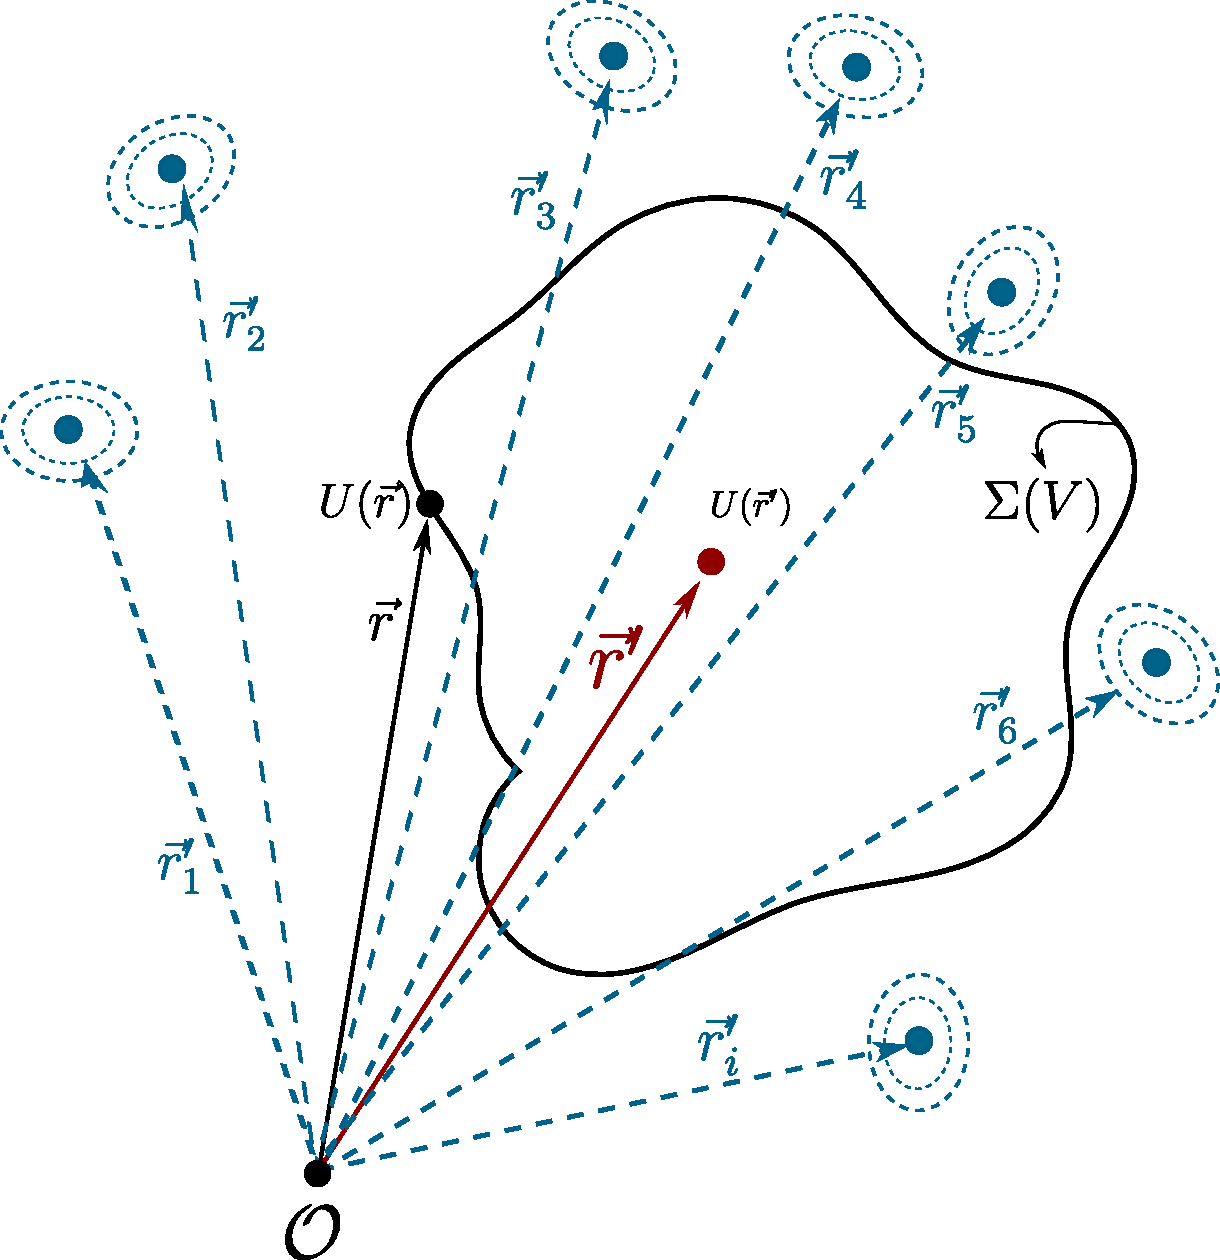
\includegraphics[width=0.7\linewidth]{Capitulo 1/Figuras/GreenImagenes}
			\caption{Sobre la frontera $\Sigma(V)$ se muestra la contribución de las componentes del campo $U(\vec{r})$; dentro de la región, el campo total se construye a partir de la contribución de todos los puntos de la frontera. Se pueden añadir infinitas cargas puntuales de Green de naturaleza de propagación arbitraria; la condición para la invariancia de la ecuación \eqref{eq:GreenHomogeneous} es que estas cargas imagen se encuentren fuera de $\Sigma(V)$.}
			\label{fig:greenimages}
		\end{figure}

		En este espíritu, la ecuación \eqref{eq:GreenHomogeneous} se convierte en
		\begin{equation}
			(\nabla^2 + k^2)G(\vec{r},\vec{r}') = -4\pi \delta(\vec{r}-\vec{r}') - 4\pi \sum_{i=1}^{\infty} \delta(\vec{r}-\vec{r}''_i).
		\end{equation}
		La solución explícita para un medio homogéneo de la ecuación \eqref{eq:GreenHomogeneous} es
		\begin{equation}
			\label{sol_Green}
			G(\vec{r}, \vec{r}') = \frac{e^{ik\|\vec{r} - \vec{r}'\|}}{\|\vec{r} - \vec{r}'\|},
		\end{equation}
		correspondiente a una onda esférica saliente centrada en $\vec{r}'$, como se demostrará en \eqref{eq:GreenSpherical}. Sustituyendo $G$ en la identidad de Green, y usando que la integral de volumen recoge el valor $-4\pi U(\vec{r}',\nu)$ debido a la delta, se obtiene
		\begin{equation}
			\label{green}
			U(\vec{r}', \nu) = -\frac{1}{4\pi} \oint_{\Sigma(V)} \left[ U(\vec{r}, \nu)\nabla G(\vec{r}, \vec{r}')- G(\vec{r}, \vec{r}')\nabla U(\vec{r}, \nu)  \right ] \cdot d\vec{\sigma},
		\end{equation}
		conocida como la fórmula integral de Helmholtz-Kirchhoff. Esta ecuación permite calcular $U(\vec{r}', \nu)$ en cualquier punto del volumen $V$ mediante una integral sobre su frontera $\Sigma(V)$.

		\begin{figure}[htbp]
			\centering
			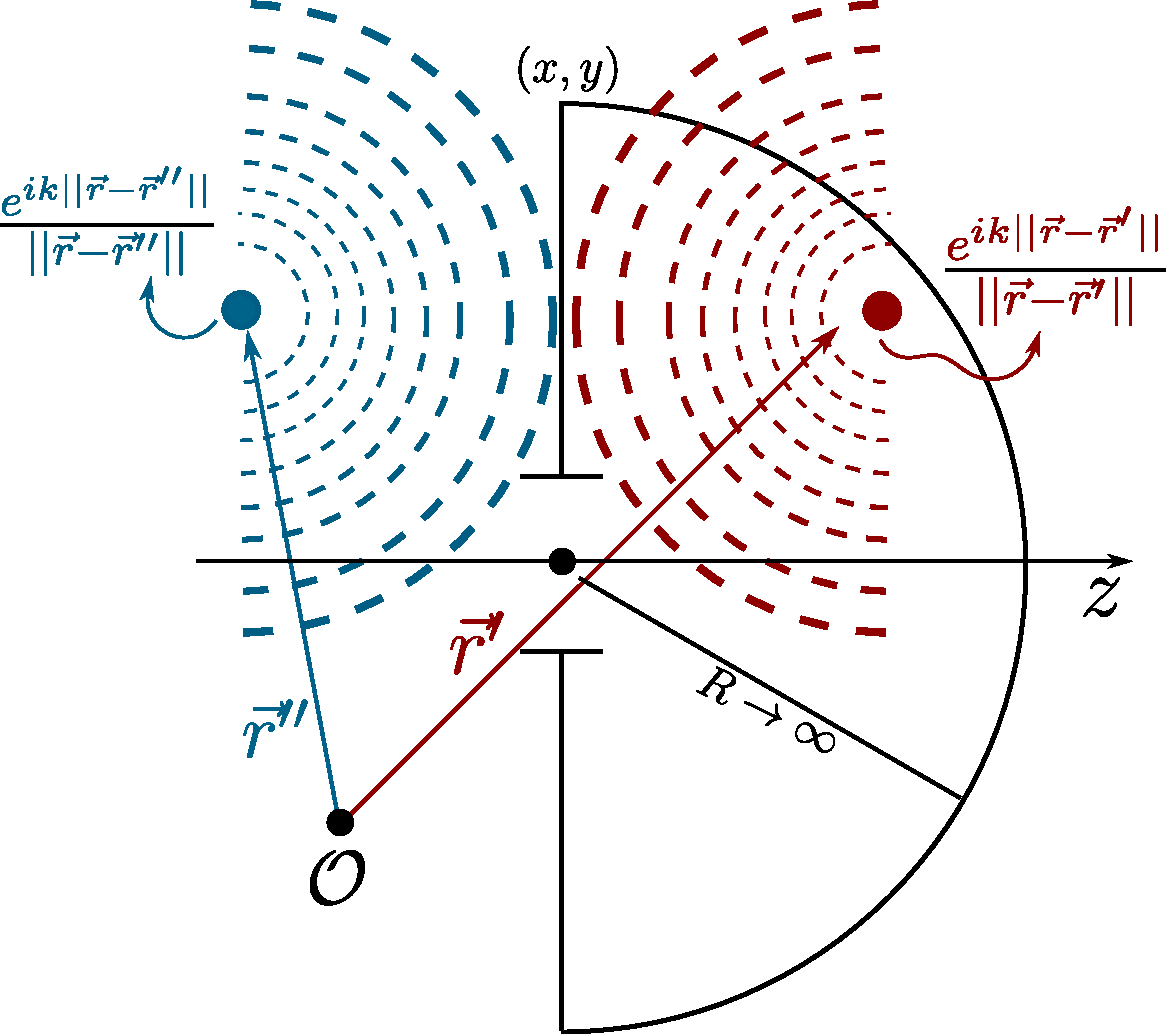
\includegraphics[width=0.7\linewidth]{Capitulo 1/Figuras/GreenPuntual}
			\caption{Representación de las funciones de Green para fuentes puntuales. Bajo estas condiciones de frontera, las funciones de Green se comportan como cargas puntuales, una imagen especular de la otra.}
			\label{fig:greenpoint}
		\end{figure}

		Antes de continuar, vale la pena notar que la naturaleza de carga puntual de las funciones de Green $G(\vec{r},\vec{r}')$ es un supuesto que se da por sentado; no existe, sin embargo, ninguna restricción sobre su naturaleza física. Como es bien sabido en la teoría electromagnética, las fuentes de radiación pueden tener cualquier volumen y forma, de modo que nuestro problema (Figura~\ref{fig:greenpoint}) puede generalizarse, como se muestra en la Figura~\ref{fig:greennonpoint}, y la ecuación diferencial para funciones de Green con volumen se leería
		\begin{equation}
			\left( \nabla^2 + k^2 \right)G(\vec{r},\vec{r}') = -4\pi \rho(\vec{r}-\vec{r}'_+) + 4\pi\rho(\vec{r}-\vec{r}'_-).
		\end{equation}

		\begin{figure}[htbp]
			\centering
			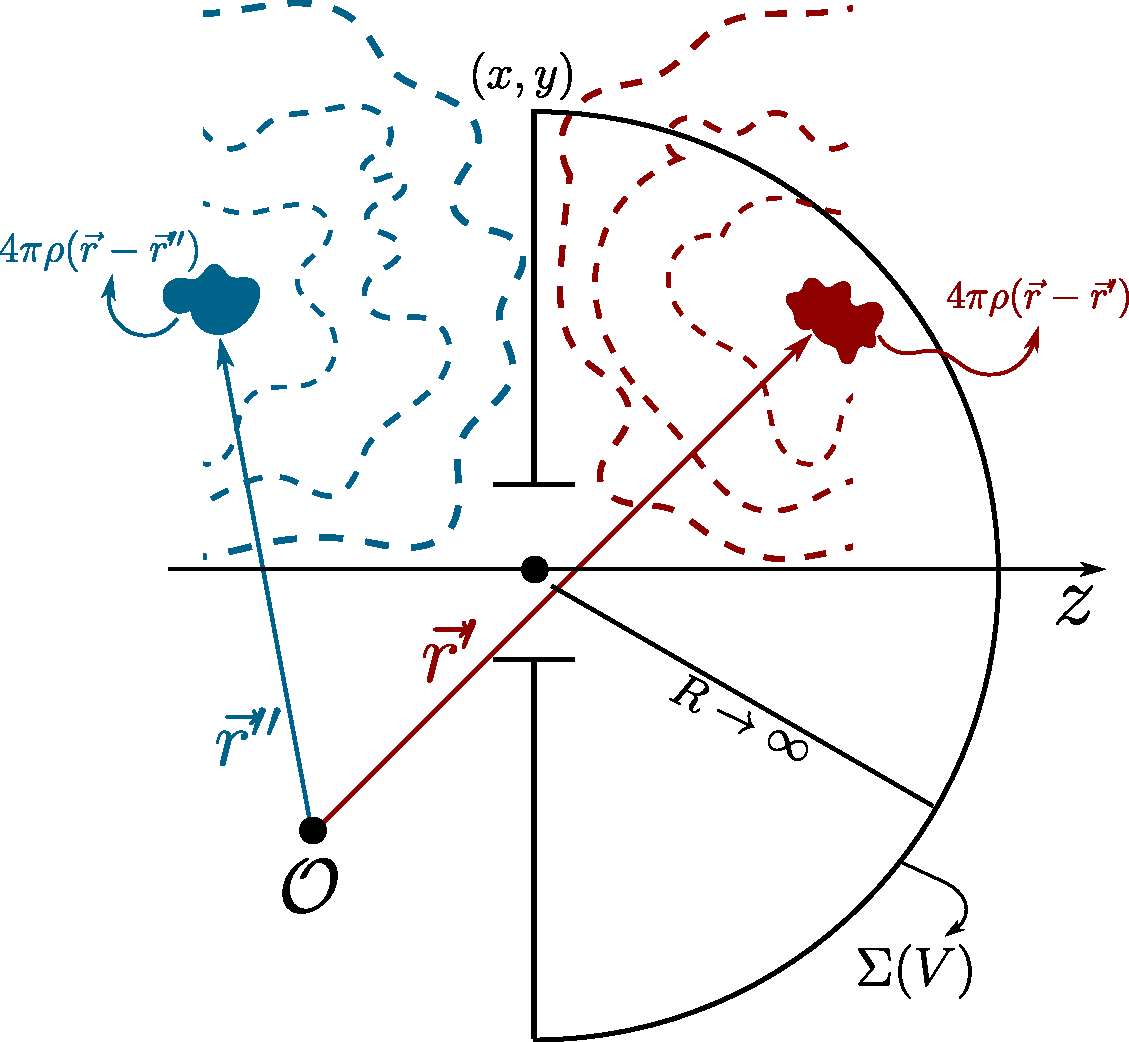
\includegraphics[width=0.7\linewidth]{Capitulo 1/Figuras/GreenNoPuntual}
			\caption{Representación de las funciones de Green para fuentes no puntuales. Bajo estas condiciones de frontera, las funciones de Green siguen comportándose como imágenes especulares, pero ahora con un volumen y una geometría dados; la única restricción sobre la emisión de estas fuentes es que, en la frontera $z=0$, el campo total debe anularse, como exigen las condiciones de Dirichlet supuestas.}
			\label{fig:greennonpoint}
		\end{figure}

		Continuemos con el desarrollo para funciones de Green puntuales. Para simplificar la evaluación de la integral, consideramos un volumen $V$ delimitado por un plano infinito $\Sigma_1$ ($z=0$) y una semiesfera $\Sigma_2$ de radio $R$ (véase la Figura~\ref{fig:greenpoint}). Cerrar la superficie en el infinito es legítimo solo si nada llega desde allí, y de nuevo esto es una decisión sobre el experimento y no una consecuencia de las matemáticas: excluye cualquier onda que converja sobre la abertura desde el lado lejano, que es precisamente lo que se dispone en el laboratorio al colocar toda fuente de luz detrás de la pantalla y al trabajar en una habitación oscurecida.

		\begin{Assumption}
			Ninguna radiación llega a la región de observación desde el infinito, siendo el campo sobre la semiesfera $\Sigma_{2}$ puramente saliente y obedeciendo la condición de radiación de Sommerfeld \eqref{eq:SommerfeldRadiation}, de modo que la contribución de $\Sigma_{2}$ se anula cuando $R\to\infty$.
		\end{Assumption}

		La fórmula de Helmholtz-Kirchhoff se reduce entonces a
		\begin{equation}
			U(\vec{r}', \nu) = -\frac{1}{4\pi} \int_{\Sigma_1} \left[U(\vec{r}, \nu)\frac{\partial G}{\partial n} -   G(\vec{r}, \vec{r}')\frac{\partial U}{\partial n} \right] d\sigma,
		\end{equation}
		donde $\frac{\partial}{\partial n} = \hat{n} \cdot \nabla$ denota la derivada normal. Sin embargo, esta formulación exige especificar simultáneamente $U$ y $\partial U/\partial n$ sobre $\Sigma_1$, lo cual sobredetermina el problema. Esta dificultad motiva la introducción de condiciones de frontera físicamente realistas, como las de Kirchhoff, para resolver la ambigüedad.

		Este problema se ve agravado por un teorema del análisis complejo, atribuido a Riemann, que afirma que si una función y su derivada normal se anulan en una región abierta de un plano, entonces la función debe ser idénticamente nula en todo el dominio. Esta restricción motiva la necesidad estratégica de eliminar uno de los términos en la integral de superficie de Helmholtz-Kirchhoff.

		La clave consiste en explotar los grados de libertad inherentes a la elección de la función de Green auxiliar $G$. Kirchhoff propuso inicialmente las condiciones de frontera intuitivas
		\begin{itemize}
			\item $U = 0$ fuera de la abertura sobre $\Sigma$ (campo bloqueado),
			\item $\partial U/\partial n = 0$ en las regiones opacas (derivada normal nula).
		\end{itemize}

		Aunque estas condiciones reproducían los resultados experimentales de la difracción, introducían inconsistencias matemáticas al violar el teorema de unicidad de Cauchy-Riemann. Poincaré mostró que tales supuestos generan contradicciones en las derivadas mixtas del campo. La resolución vino de Sommerfeld, quien redefinió $G$ por medio de una función de Green de doble capa (especular), garantizando que
		\begin{itemize}
			\item $G = 0$ sobre $\Sigma$ (condición de Dirichlet),
			\item $\partial G/\partial n$ permanece no singular,
		\end{itemize}

	eliminando así la redundancia en las condiciones de frontera y preservando la autoconsistencia del formalismo.

	El artificio de Sommerfeld elimina uno de los dos términos de frontera, pero no elimina la necesidad de conocer el que sobrevive. La fórmula de Rayleigh-Sommerfeld sigue requiriendo el valor de $U$ en cada punto del plano $\Sigma_{1}$, y ninguna teoría de la difracción puede suministrarlo, porque obtenerlo significaría resolver exactamente el problema electromagnético de la pantalla que precisamente buscábamos evitar. Lo que se hace en cambio es adivinarlo, y la conjetura es la de Kirchhoff. Descansa sobre dos idealizaciones separadas, una sobre el obstáculo y otra sobre el campo en él, y ambas merecen enunciarse como lo que son.

	\begin{Assumption}
		La pantalla es un obstáculo plano de espesor nulo, perfectamente opaco y perfectamente absorbente, cuyas propiedades materiales no desempeñan ningún papel en el problema y cuyos bordes no perturban el campo en su vecindad.
	\end{Assumption}

	\begin{Assumption}
		Sobre la abertura el campo coincide con el campo que existiría si la pantalla nunca se hubiera introducido, y sobre la parte opaca de la pantalla se anula idénticamente.
	\end{Assumption}

	El segundo de estos supuestos es el eslabón más débil de toda la construcción, y resulta instructivo ver por qué. Un campo que se anula en parte de un plano y coincide con una onda incidente suave en el resto es discontinuo en el borde de la abertura, por lo que no puede ser una solución exacta de la ecuación de Helmholtz; los valores de frontera que prescribimos son, estrictamente hablando, incompatibles con la ecuación que estamos resolviendo. El error queda confinado a un borde de unas pocas longitudes de onda de ancho alrededor del borde, razón por la cual la teoría funciona tan bien para aberturas de muchas longitudes de onda y falla para aberturas comparables con la longitud de onda.


	\subsection{La formulación de Rayleigh-Sommerfeld}

		Ya hemos usado dos veces la forma explícita \eqref{sol_Green} de la función de Green sin justificarla, y puesto que toda la construcción de Rayleigh-Sommerfeld descansa tanto en la forma de esa función como en la libertad de sumarle una segunda, este es el lugar para mostrar de dónde proviene.

		\begin{myteo}
			Sea $R = \|\vec{r}-\vec{r}'\|$. En un medio homogéneo, isótropo e ilimitado, la única solución de la ecuación de Green \eqref{eq:GreenHomogeneous} que transporta energía alejándose de la fuente es la onda esférica saliente
			\begin{equation}\label{eq:GreenSpherical}
				G(\vec{r},\vec{r}') = \frac{e^{ikR}}{R},
			\end{equation}
			fijándose su amplitud por la intensidad asignada al emisor puntual y quedando excluida la solución convergente por la condición de radiación.
		\end{myteo}

		La demostración tiene cuatro pasos, y cada uno de ellos es una afirmación física antes de ser una afirmación matemática. El primero es una cuestión de simetría. El medio es homogéneo e isótropo y la fuente es un único punto, de modo que, una vez colocado el origen en $\vec{r}'$, nada en el problema distingue una dirección del espacio de otra; la solución solo puede depender de la distancia $R$ a la fuente, y podemos escribir $G = G(R)$.

		El segundo paso consiste en resolver la ecuación lejos de la fuente, donde es homogénea. Para una función que depende únicamente de $R$, el laplaciano se reduce a
		\begin{equation}\label{eq:GreenRadialLaplacian}
			\nabla^{2}G = \frac{1}{R^{2}}\frac{d}{dR}\left(R^{2}\frac{dG}{dR}\right) = \frac{1}{R}\frac{d^{2}}{dR^{2}}\left(R\,G\right),
		\end{equation}
		donde la segunda forma corresponde a una identidad radial ya establecida al estudiar el laplaciano en coordenadas esféricas, y que sugiere de inmediato la sustitución $\chi(R) = R\,G(R)$. Con ella, la ecuación de Helmholtz homogénea se convierte en
		\begin{equation}\label{eq:RadialOscillator}
			\frac{d^{2}\chi}{dR^{2}} + k^{2}\chi = 0 ,
		\end{equation}
		que es la ecuación de un oscilador armónico en la variable $R$ y cuya solución general es $\chi = A\,e^{ikR} + B\,e^{-ikR}$. Deshaciendo la sustitución,
		\begin{equation}\label{eq:GreenGeneralRadial}
			G(R) = A\,\frac{e^{ikR}}{R} + B\,\frac{e^{-ikR}}{R},
		\end{equation}
		de modo que la amplitud de un campo monocromático con simetría esférica decae necesariamente como el inverso de la distancia. Esto no es un accidente del álgebra. La energía que atraviesa una esfera de radio $R$ es proporcional a $|G|^{2}R^{2}$, y solo con la dependencia $1/R$ esta cantidad resulta independiente de $R$, tal como exige la conservación de la energía en un medio transparente.

		El tercer paso selecciona entre los dos términos de \eqref{eq:GreenGeneralRadial}. Restaurando el factor temporal de la convención de Fourier adoptada en \eqref{eq.FT}, las dos soluciones se leen $e^{i(kR-\omega t)}/R$ y $e^{-i(kR+\omega t)}/R$, y sus superficies de fase constante obedecen respectivamente $R = ct + \text{const}$ y $R = -ct + \text{const}$. La primera se expande y la segunda se contrae. Nuestro punto es un emisor y no un sumidero, y la luz debe alejarse de él y nunca regresar, que es el contenido físico de la condición de radiación de Sommerfeld ya invocada al descartar la semiesfera $\Sigma_{2}$,
		\begin{equation}\label{eq:SommerfeldRadiation}
			\lim_{R\to\infty} R\left(\frac{\partial G}{\partial R} - ikG\right) = 0 .
		\end{equation}
		La onda convergente la viola, pues para ella el corchete se comporta como $-2ikB\,e^{-ikR}/R$ y el producto con $R$ no tiende a cero. Por lo tanto $B = 0$.

		El cuarto paso es el único en el que interviene la delta, y es el que fija la amplitud $A$. Integramos \eqref{eq:GreenHomogeneous} sobre la bola $B_{\varepsilon}$ de radio $\varepsilon$ centrada en la fuente, que es lo que produjo \eqref{eq:GreenFlux}. Con $G = A\,e^{ikR}/R$ el término de volumen está acotado por
		\begin{equation*}
			\left|k^{2}\int_{B_{\varepsilon}} G\, dV\right| = \left|4\pi A k^{2}\int_{0}^{\varepsilon} \frac{e^{ikR}}{R}\,R^{2}\,dR\right| \leq 2\pi |A|\,k^{2}\varepsilon^{2} \xrightarrow[\varepsilon\to 0]{} 0,
		\end{equation*}
		de modo que la singularidad de $G$ es lo suficientemente suave para ser integrable, y toda la intensidad de la fuente debe provenir del término de flujo. Puesto que $\partial G/\partial R = A\,e^{ikR}\left(ik/R - 1/R^{2}\right)$, y la esfera $\partial B_{\varepsilon}$ tiene área $4\pi\varepsilon^{2}$ con normal exterior $\hat{R}$,
		\begin{equation*}
			\oint_{\partial B_{\varepsilon}} \nabla G\cdot d\vec{\sigma} = 4\pi\varepsilon^{2}\,A\,e^{ik\varepsilon}\left(\frac{ik}{\varepsilon}-\frac{1}{\varepsilon^{2}}\right) = 4\pi A\,e^{ik\varepsilon}\left(ik\varepsilon - 1\right) \xrightarrow[\varepsilon\to 0]{} -4\pi A ,
		\end{equation*}
		y \eqref{eq:GreenFlux} da entonces $-4\pi A = -4\pi$, es decir $A = 1$, lo que demuestra \eqref{eq:GreenSpherical} y completa el argumento.

		El signo de la fuente merece un comentario, porque es la razón por la cual \eqref{eq:GreenHomogeneous} lleva $-4\pi$ y no $+4\pi$ en el lado derecho. El último paso de la demostración muestra que el flujo de $\nabla G$ que sale de una pequeña esfera es $-4\pi A$, de modo que una amplitud positiva $A$ exige una constante negativa en la ecuación; si hubiéramos escrito $+4\pi\delta(\vec{r}-\vec{r}')$ nos habríamos visto obligados a aceptar $A = -1$, es decir $G = -e^{ikR}/R$, y toda fórmula escrita a partir de \eqref{sol_Green} en adelante habría cambiado de signo. La convención adoptada aquí es la usada por Sommerfeld, Born y Wolf, y Goodman \citep{sommerfeld1954optics, born1999principles, goodman2005introduction}, y es la convención para la cual la integral de difracción resulta con la conocida constante $1/(i\lambda)$. Lo que el cálculo establece, más allá de la contabilidad de signos, es que la solución elemental es una onda esférica saliente centrada en el punto fuente cuya amplitud es inversamente proporcional a la distancia. Esta es la ondita de Huygens, ahora obtenida en lugar de supuesta.

		Volviendo a la ecuación \eqref{green} y eligiendo la condición de Dirichlet para la función $G$, el segundo término del integrando desaparece y nos queda
		\begin{equation}
			\label{psi_expr}
			U(\vec{r}', \nu) = -\frac{1}{4\pi} \int_{\Sigma_1} \left[U(\vec{r}, \nu) \nabla G \cdot\hat{n}\right] d\sigma .
		\end{equation}
		Aquí $\hat{n}$ es la normal que apunta \textit{hacia afuera} de $V$, y como $V$ es el semiespacio $z>0$, sobre el plano $\Sigma_{1}$ esa normal apunta hacia abajo, $\hat{n} = -\hat{z}$. Vale la pena escribir esto explícitamente, porque es el signo que con mayor facilidad se pierde en toda la construcción,
		\begin{equation}\label{eq:RSnormal}
			U(\vec{r}', \nu) = \frac{1}{4\pi} \int_{\Sigma_1} U(\vec{r}, \nu)\,\nabla G \cdot\hat{z}\; d\sigma .
		\end{equation}
		Dada la superficie de integración considerada, podemos expresar \eqref{sol_Green} como
		\begin{equation}
			\label{sol_Green_RS}
			G(\vec{r}, \vec{r}') = \frac{e^{ik\|\vec{r} - \vec{r}'\|}}{\|\vec{r} - \vec{r}'\|} - \frac{e^{ik\|\vec{r} - \vec{r}''\|}}{\|\vec{r} - \vec{r}''\|},
		\end{equation}
		\noindent donde
		\begin{align}
			\|\vec{r} - \vec{r}''\| &= \|\vec{r} - \vec{r}'\|, \qquad x'' = x', \quad y'' = y', \quad z'' = -z',
		\end{align}
		puesto que $\vec{r}''$ es la imagen especular de $\vec{r}'$ respecto al plano $\Sigma_1$.

		Que \eqref{sol_Green_RS} sea una función de Green legítima se verifica de inmediato con el teorema recién demostrado. El punto de observación $\vec{r}'$ se encuentra en el semiespacio $z>0$, de modo que su imagen $\vec{r}''$ se encuentra en $z<0$, fuera del volumen $V$; dentro de $V$, el segundo término es entonces una solución perfectamente regular de la ecuación de Helmholtz homogénea, y sumarlo no altera ni la fuente en $\vec{r}'$ ni el valor de la integral de volumen, de acuerdo con la libertad discutida después de \eqref{eq:GreenHomogeneous}. Sobre el plano $\Sigma_{1}$, en cambio, todo punto es equidistante de $\vec{r}'$ y de $\vec{r}''$, de modo que las dos ondas esféricas llegan allí con la misma amplitud y la misma fase y se cancelan idénticamente, dando $G = 0$ en todo $\Sigma_{1}$. Esta es la condición de Dirichlet que buscábamos, obtenida mediante el mismo método de imágenes que resuelve el interferómetro de Michelson, y es lo que elimina el término en $\partial U/\partial n$ de \eqref{green} y con él la sobredeterminación de las condiciones de frontera de Kirchhoff.

		Todo lo que \eqref{eq:RSnormal} sigue requiriendo es la derivada axial de $G$ sobre el plano. Este es el único cálculo de la sección, y puesto que un signo perdido aquí cambia el signo de toda fórmula de difracción del resto del capítulo, lo llevaremos a cabo sin omitir un solo paso. Para aligerar la notación escribimos
		\begin{equation}\label{eq:RSDistances}
			r_{1} = \|\vec{r}-\vec{r}'\|, \qquad r_{2} = \|\vec{r}-\vec{r}''\|, \qquad f(\rho) = \dfrac{e^{ik\rho}}{\rho},
		\end{equation}
		de modo que \eqref{sol_Green_RS} se lee simplemente $G = f(r_{1}) - f(r_{2})$.

		\textit{Primer paso: la derivada de $f$.} Derivando el cociente,
		\begin{equation}\label{eq:RSderivf}
			\dfrac{df}{d\rho} = \dfrac{\left(ik\,e^{ik\rho}\right)\rho - e^{ik\rho}}{\rho^{2}} = \dfrac{e^{ik\rho}}{\rho}\left(ik - \dfrac{1}{\rho}\right) = \left(ik-\dfrac{1}{\rho}\right)f(\rho).
		\end{equation}

		\textit{Segundo paso: el gradiente de una distancia.} Con $\vec{r} = (x,y,z)$ el punto de integración y $\vec{r}' = (x',y',z')$ fijo,
		\begin{equation}\label{eq:RSr1}
			r_{1} = \left[(x-x')^{2}+(y-y')^{2}+(z-z')^{2}\right]^{1/2},
		\end{equation}
		y derivando respecto a $z$, que es la única componente que necesitaremos,
		\begin{equation}\label{eq:RSdr1dz}
			\dfrac{\partial r_{1}}{\partial z} = \dfrac{1}{2}\,\dfrac{2\left(z-z'\right)}{\left[(x-x')^{2}+(y-y')^{2}+(z-z')^{2}\right]^{1/2}} = \dfrac{z-z'}{r_{1}} ,
		\end{equation}
		el mismo cálculo con $\vec{r}''$ en lugar de $\vec{r}'$ da $\partial r_{2}/\partial z = (z-z'')/r_{2}$. Realizado para las tres componentes a la vez, estos dos resultados se leen $\nabla r_{1} = (\vec{r}-\vec{r}')/r_{1}$ y $\nabla r_{2} = (\vec{r}-\vec{r}'')/r_{2}$: el gradiente de una distancia es el vector unitario que apunta alejándose del centro desde el cual se mide la distancia.

		\textit{Tercer paso: el gradiente de $G$.} Aplicando la regla de la cadena a cada término y usando \eqref{eq:RSderivf},
		\begin{equation}\label{eq:RSgradG}
			\nabla G = \left(ik-\dfrac{1}{r_{1}}\right)\dfrac{e^{ikr_{1}}}{r_{1}}\,\dfrac{\vec{r}-\vec{r}'}{r_{1}} \;-\; \left(ik-\dfrac{1}{r_{2}}\right)\dfrac{e^{ikr_{2}}}{r_{2}}\,\dfrac{\vec{r}-\vec{r}''}{r_{2}} .
		\end{equation}

		\textit{Cuarto paso: la proyección sobre el eje.} Tomando el producto escalar de \eqref{eq:RSgradG} con $\hat{z}$, lo cual equivale a conservar la tercera componente de cada uno de los dos vectores,
		\begin{equation}\label{eq:RSgradGz}
			\nabla G\cdot\hat{z} = \left(ik-\dfrac{1}{r_{1}}\right)\dfrac{e^{ikr_{1}}}{r_{1}}\,\dfrac{z-z'}{r_{1}} \;-\; \left(ik-\dfrac{1}{r_{2}}\right)\dfrac{e^{ikr_{2}}}{r_{2}}\,\dfrac{z-z''}{r_{2}} .
		\end{equation}

		\textit{Quinto paso: evaluación sobre el plano.} La integral de \eqref{eq:RSnormal} se extiende sobre $\Sigma_{1}$, de modo que \eqref{eq:RSgradGz} solo se necesita en $z=0$. Allí las dos distancias coinciden, $r_{1} = r_{2} \equiv r$, que es la relación especular ya usada, y los dos desplazamientos axiales son
		\begin{equation}\label{eq:RSopposite}
			\left.\left(z-z'\right)\right|_{z=0} = -z', \qquad \left.\left(z-z''\right)\right|_{z=0} = -z'' = z' ,
		\end{equation}
		porque $z'' = -z'$. Este es el punto crucial de todo el cálculo: la fuente y su imagen se encuentran en lados opuestos del plano, de modo que sus cosenos directores axiales son iguales en magnitud y opuestos en signo. Sustituyendo \eqref{eq:RSopposite} en \eqref{eq:RSgradGz}, el factor común $\left(ik-1/r\right)e^{ikr}/r$ puede extraerse y lo que queda es una diferencia de dos números opuestos,
		\begin{equation}\label{eq:RSgradGplane}
			\left.\nabla G\cdot\hat{z}\right|_{\Sigma_{1}} = \left(ik-\dfrac{1}{r}\right)\dfrac{e^{ikr}}{r}\left[\dfrac{-z'}{r} - \dfrac{z'}{r}\right] = -\,\dfrac{2z'}{r}\left(ik-\dfrac{1}{r}\right)\dfrac{e^{ikr}}{r} .
		\end{equation}
		El factor dos merece un comentario. El signo menos que separa los dos términos de \eqref{sol_Green_RS} es lo que hace que las dos ondas esféricas se cancelen sobre el plano; ese mismo signo menos, combinado con los cosenos directores opuestos de \eqref{eq:RSopposite}, hace que sus derivadas axiales se sumen. La función de Green de Dirichlet se anula sobre $\Sigma_{1}$ y tiene allí exactamente el doble de la derivada normal de una única ondita, que es la huella analítica del hecho de que la pantalla se comporta como un espejo perfecto.

		\textit{Sexto paso: el factor de oblicuidad.} Solo resta nombrar la cantidad geométrica $z'/r$. Sea $\theta$ el ángulo entre el eje $\hat{z}$ y el vector $\vec{r}\,'-\vec{r}$ que va del punto de la abertura al punto de observación, de modo que
		\begin{equation}\label{eq:RSobliquity}
			\cos\theta = \hat{z}\cdot\dfrac{\vec{r}\,'-\vec{r}}{\|\vec{r}\,'-\vec{r}\|} = \dfrac{z'}{r} ,
		\end{equation}
		cantidad que es positiva porque el punto de observación se encuentra en $z>0$, y que es igual a uno para un punto de la abertura situado sobre el eje de observación. Con esta notación, \eqref{eq:RSgradGplane} adopta su forma final,
		\begin{equation}\label{eq:RSnormalDerivative}
			\left.\nabla G\cdot\hat{z}\right|_{\Sigma_{1}} = -2\left[ik-\dfrac{1}{r}\right]\dfrac{e^{ikr}}{r}\,\cos\theta .
		\end{equation}
		Es esencial tener presente desde cuál de los dos vectores se mide el ángulo. Si hubiéramos escrito el coseno director de $\vec{r}-\vec{r}'$, que apunta desde el punto de observación de vuelta a la abertura, habríamos obtenido el número opuesto, y la integral de difracción habría resultado con el signo equivocado.

		Sustituyendo \eqref{eq:RSnormalDerivative} en \eqref{eq:RSnormal}, los dos factores de dos se combinan con el $4\pi$ y obtenemos
		\begin{equation}\label{eq:RSexact}
			U(\vec{r}',\nu) = -\dfrac{1}{2\pi} \int_{\Sigma} U(\vec{r},\nu) \left[ik - \dfrac{1}{\|\vec{r} - \vec{r}'\|} \right] \dfrac{e^{ik\|\vec{r}-\vec{r}'\|}}{\|\vec{r}-\vec{r}'\|} \cos\theta\,d\sigma .
		\end{equation}
		La ecuación \eqref{eq:RSexact} es exacta dentro de la teoría escalar, y es la última expresión de este capítulo de la que puede decirse esto. Para llevarla a la forma en que efectivamente se usa, se descarta el término $1/\|\vec{r}-\vec{r}'\|$ frente a $k$, lo cual solo es lícito cuando el punto de observación se encuentra a muchas longitudes de onda de la abertura. Para luz visible y distancias de laboratorio, la razón descartada $\lambda/(2\pi\|\vec{r}-\vec{r}'\|)$ es del orden de $10^{-7}$, de modo que la aproximación es excelente, pero es una aproximación y no una identidad.

		\begin{Assumption}
			El punto de observación se encuentra a muchas longitudes de onda de todo punto de la abertura, $\|\vec{r}-\vec{r}'\| \gg \lambda$, de modo que el término de campo cercano $1/\|\vec{r}-\vec{r}'\|$ es despreciable frente al número de onda $k$.
		\end{Assumption}

		Con ello obtenemos
		\begin{equation}\label{eq:RSfinal}
			U(\vec{r}',\nu) = -\dfrac{ik}{2\pi} \int_{\Sigma} U(\vec{r},\nu)\dfrac{e^{ik\|\vec{r}-\vec{r}'\|}}{\|\vec{r}-\vec{r}'\|} \cos\theta\,d\sigma = \dfrac{1}{i\lambda} \int_{\Sigma} U(\vec{r},\nu)\dfrac{e^{ik\|\vec{r}-\vec{r}'\|}}{\|\vec{r}-\vec{r}'\|} \cos\theta\,d\sigma,
		\end{equation}
		donde la última igualdad no es otra cosa que $-ik/2\pi = -i/\lambda = 1/(i\lambda)$. Esta es una expresión matemática que encarna el principio de Huygens-Fresnel: como puede apreciarse, hay una onda esférica por cada punto de la superficie de integración, ponderada por el factor de oblicuidad $\cos\theta$ y por la constante $1/(i\lambda)$, que es la constante que Fresnel tuvo que postular y que la derivación ahora entrega, con avance de cuarto de onda y $1/\lambda$ incluidos.

\section{La aproximación de Fresnel}

Partiendo del campo
\begin{align}
	U(\vec{r}') = -\frac{ik}{2\pi}\int_{\Sigma} U(\vec{r}) \frac{e^{ik \left\| \vec{r} - \vec{r}' \right\|}}{\left\| \vec{r} - \vec{r}' \right\|} \cos\theta \, \mathrm{d}\sigma,
\end{align}
es posible llevar a cabo la llamada aproximación de campo medio, o de Fresnel. La expansión sobre la que descansa es de tipo binomial, y una serie binomial solo puede truncarse cuando la cantidad expandida es pequeña; aquí esa cantidad es la razón entre la separación transversal y la distancia de propagación, de modo que truncar equivale a confinar todo el problema a un cono estrecho alrededor del eje óptico.

\begin{Assumption}
	Las dimensiones transversales de la abertura y de la región de observación son pequeñas comparadas con la distancia de propagación $z'$, y el término cuártico omitido en la expansión contribuye con una fase muy por debajo de un radián, $k\left[(x-x')^{2}+(y-y')^{2}\right]^{2}/8z'^{3} \ll 1$.
\end{Assumption}

Para ello recordamos que la integración se extiende sobre el plano $\Sigma_{1}$, en el cual $z=0$, de modo que la separación axial entre los dos puntos es la coordenada $z'$ del punto de observación por sí sola,
\begin{align}
	\label{aprox_r}
	\|\vec{r}-\vec{r}'\| &= \left.\left[(x-x')^2 + (y-y')^2 + (z-z')^2\right]^{1/2}\right|_{z=0} \notag \\
	&= \left[(x-x')^2 + (y-y')^2 + z'^2\right]^{1/2} \notag \\
	&= z'\left(1 + \dfrac{(x-x')^2 + (y-y')^2}{z'^2} \right)^{1/2} \notag \\
	&\approx z' + \dfrac{(x-x')^2+(y-y')^2}{2z'}.
\end{align}
Es $z'$, y no $z$, lo que mide la distancia de propagación. La abertura se encuentra en el origen del eje y es el punto de observación el que se desplaza, lo cual es la misma convención que produjo el factor de oblicuidad $\cos\theta = z'/r$ de \eqref{eq:RSobliquity} y la evaluación en $z=0$ de \eqref{eq:RSopposite}. Fijar $z'=0$ y factorizar $z$ en su lugar colocaría el punto de observación sobre la pantalla y haría que la distancia de propagación se anulara idénticamente.
Resulta claro que, para el factor $\dfrac{1}{\|\vec{r}- \vec{r}'\|}$, basta una expansión hasta el primer término de \eqref{aprox_r}; esto no basta, sin embargo, para el factor $e^{ik \left\| \vec{r} - \vec{r}' \right\|}$, ya que este último tiene comportamiento oscilatorio en su dominio, de modo que se requieren ambos términos. Los dos factores se tratan, por lo tanto, con distintos grados de precisión, y esa asimetría es en sí misma una hipótesis: presupone que un error de una fracción de longitud de onda, inofensivo en una amplitud que varía lentamente, es fatal en una fase, lo cual es cierto precisamente porque $k$ es enorme en la escala de la abertura.

\begin{Assumption}
	En la amplitud, la distancia puede reemplazarse por la separación axial, $\|\vec{r}-\vec{r}'\| \approx z'$, mientras que en la fase debe conservarse el término cuadrático de \eqref{aprox_r}.
\end{Assumption}

Tomamos además, para el factor de oblicuidad \eqref{eq:RSobliquity}, $\cos\theta = \dfrac{z'}{\|\vec{r} - \vec{r} '\|} \approx 1$, lo cual es lícito en el régimen paraxial porque el punto de observación se encuentra entonces cerca del eje.

\begin{Assumption}
	El factor de oblicuidad es unitario, $\cos\theta \approx 1$, formando toda dirección de interés un ángulo pequeño con el eje óptico.
\end{Assumption}

En este espíritu, obtenemos una expresión para el campo de la forma
\begin{equation}
	\label{Fresnel}
	U(\vec{r}') = \dfrac{e^{ikz'}}{i\lambda z'} \int U(\vec{r}) \exp \left(\dfrac{ik}{2z'} ((x-x')^2 + (y-y')^2) \right) d\sigma,
\end{equation}
que describe la propagación o difracción del campo electromagnético en el régimen de Fresnel. La constante $1/(i\lambda z')$, heredada de \eqref{eq:RSfinal}, es aquella para la cual el núcleo de \eqref{Fresnel} tiende a $\delta(\vec{r}-\vec{r}\,')$ cuando $z'\to 0$, de modo que una propagación a distancia nula deja el campo inalterado; esta es la comprobación que fija el signo sin lugar a dudas. Vale la pena subrayar que la ecuación \eqref{Fresnel} describe una onda parabólica, y aunque, al menos conceptualmente, tal propagación es válida para un campo medio, en la práctica ha resultado más que suficiente para distancias suficientemente cortas.

	\subsection{Ejemplo: difracción de Fraunhofer entre dos esferas confocales}

		\textit{Partiendo de la integral de Fresnel \eqref{Fresnel}, mostrar que entre dos esferas confocales se obtiene difracción de Fraunhofer.}

		Ante todo conviene expandir el cuadrado en el exponente de \eqref{Fresnel}. Escribiendo $r^{2} = x^{2}+y^{2}$ para el radio transversal en el plano emisor y $r'^{2} = x'^{2}+y'^{2}$ para el del plano receptor,
		\begin{equation}\label{eq:ExpandFresnelSquare}
			(x-x')^{2} + (y-y')^{2} = r^{2} + r'^{2} - 2\left(xx'+yy'\right),
		\end{equation}
		de modo que la integral de Fresnel se separa en tres factores,
		\begin{equation}\label{eq:FresnelThreeFactors}
			U(\vec{r}\,') = \dfrac{e^{ikz'}}{i\lambda z'}\int U(\vec{r})\,
			e^{\frac{ik}{2z'}r^{2}}\;
			e^{\frac{ik}{2z'}r'^{2}}\;
			e^{-\frac{ik}{z'}\left(xx'+yy'\right)}\,d\sigma .
		\end{equation}
		El último factor ya es el núcleo de una transformación de Fourier. El obstáculo es el par de factores cuadráticos, y todo el sentido del ejercicio es que no son obstáculo en absoluto si se acepta leer el campo sobre una superficie curva en lugar de sobre un plano.

		Consideremos un casquete esférico tangente a un plano transversal en el eje óptico, con su centro de curvatura sobre el eje a la distancia con signo $c$ desde el vértice, contada positiva en la dirección de propagación. El punto del casquete en la posición transversal $\vec{r}$ está desplazado axialmente respecto al plano tangente por la sagita
		\begin{align*}
			& \delta(r) = c - \operatorname{sgn}(c)\sqrt{c^{2}-r^{2}} = c - \operatorname{sgn}(c)\,|c|\sqrt{1-\dfrac{r^{2}}{c^{2}}} \approx {\color{red}c} - {\color{red}c}\left(1 - \dfrac{r^{2}}{2c^{2}}\right),
		\end{align*}
		donde usamos $\operatorname{sgn}(c)\,|c| = c$ y expandimos la raíz a primer orden, que es la misma expansión paraxial ya realizada en \eqref{aprox_r}. Los dos términos en rojo se cancelan y queda
		\begin{equation}\label{eq:ConfocalSagitta}
			\delta(r) = \dfrac{r^{2}}{2c}.
		\end{equation}
		Puesto que un campo que se propaga en la dirección positiva adquiere el factor $e^{ik\delta}$ a lo largo de un desplazamiento axial $\delta$, el campo leído sobre el casquete y el campo leído sobre el plano tangente están relacionados por
		\begin{equation}\label{eq:ConfocalRule}
			u_{\text{cap}}(\vec{r}) = U(\vec{r})\exp\left(\dfrac{ik\,r^{2}}{2c}\right).
		\end{equation}

		Se dice que dos esferas son \textit{confocales} cuando cada una tiene su centro de curvatura en el vértice de la otra. Sea entonces $\mathcal{A}$ el casquete tangente al plano emisor $\mathcal{P}$ en el vértice $O$ y centrado en $O'$, y sea $\mathcal{F}$ el casquete tangente al plano receptor $\mathcal{Q}$ en el vértice $O'$ y centrado en $O$, como se muestra en la Figura~\ref{fig:ConfocalSpheres}. Ambos radios son entonces iguales a la distancia de propagación, y con la convención de signos de \eqref{eq:ConfocalRule} las dos distancias con signo son
		\begin{equation}\label{eq:ConfocalRadii}
			c_{\mathcal{A}} = +z', \qquad c_{\mathcal{F}} = -z',
		\end{equation}
		siendo la segunda negativa porque el centro de $\mathcal{F}$ se encuentra aguas arriba de su propio vértice.

		\begin{figure}[!ht]
			\centering
			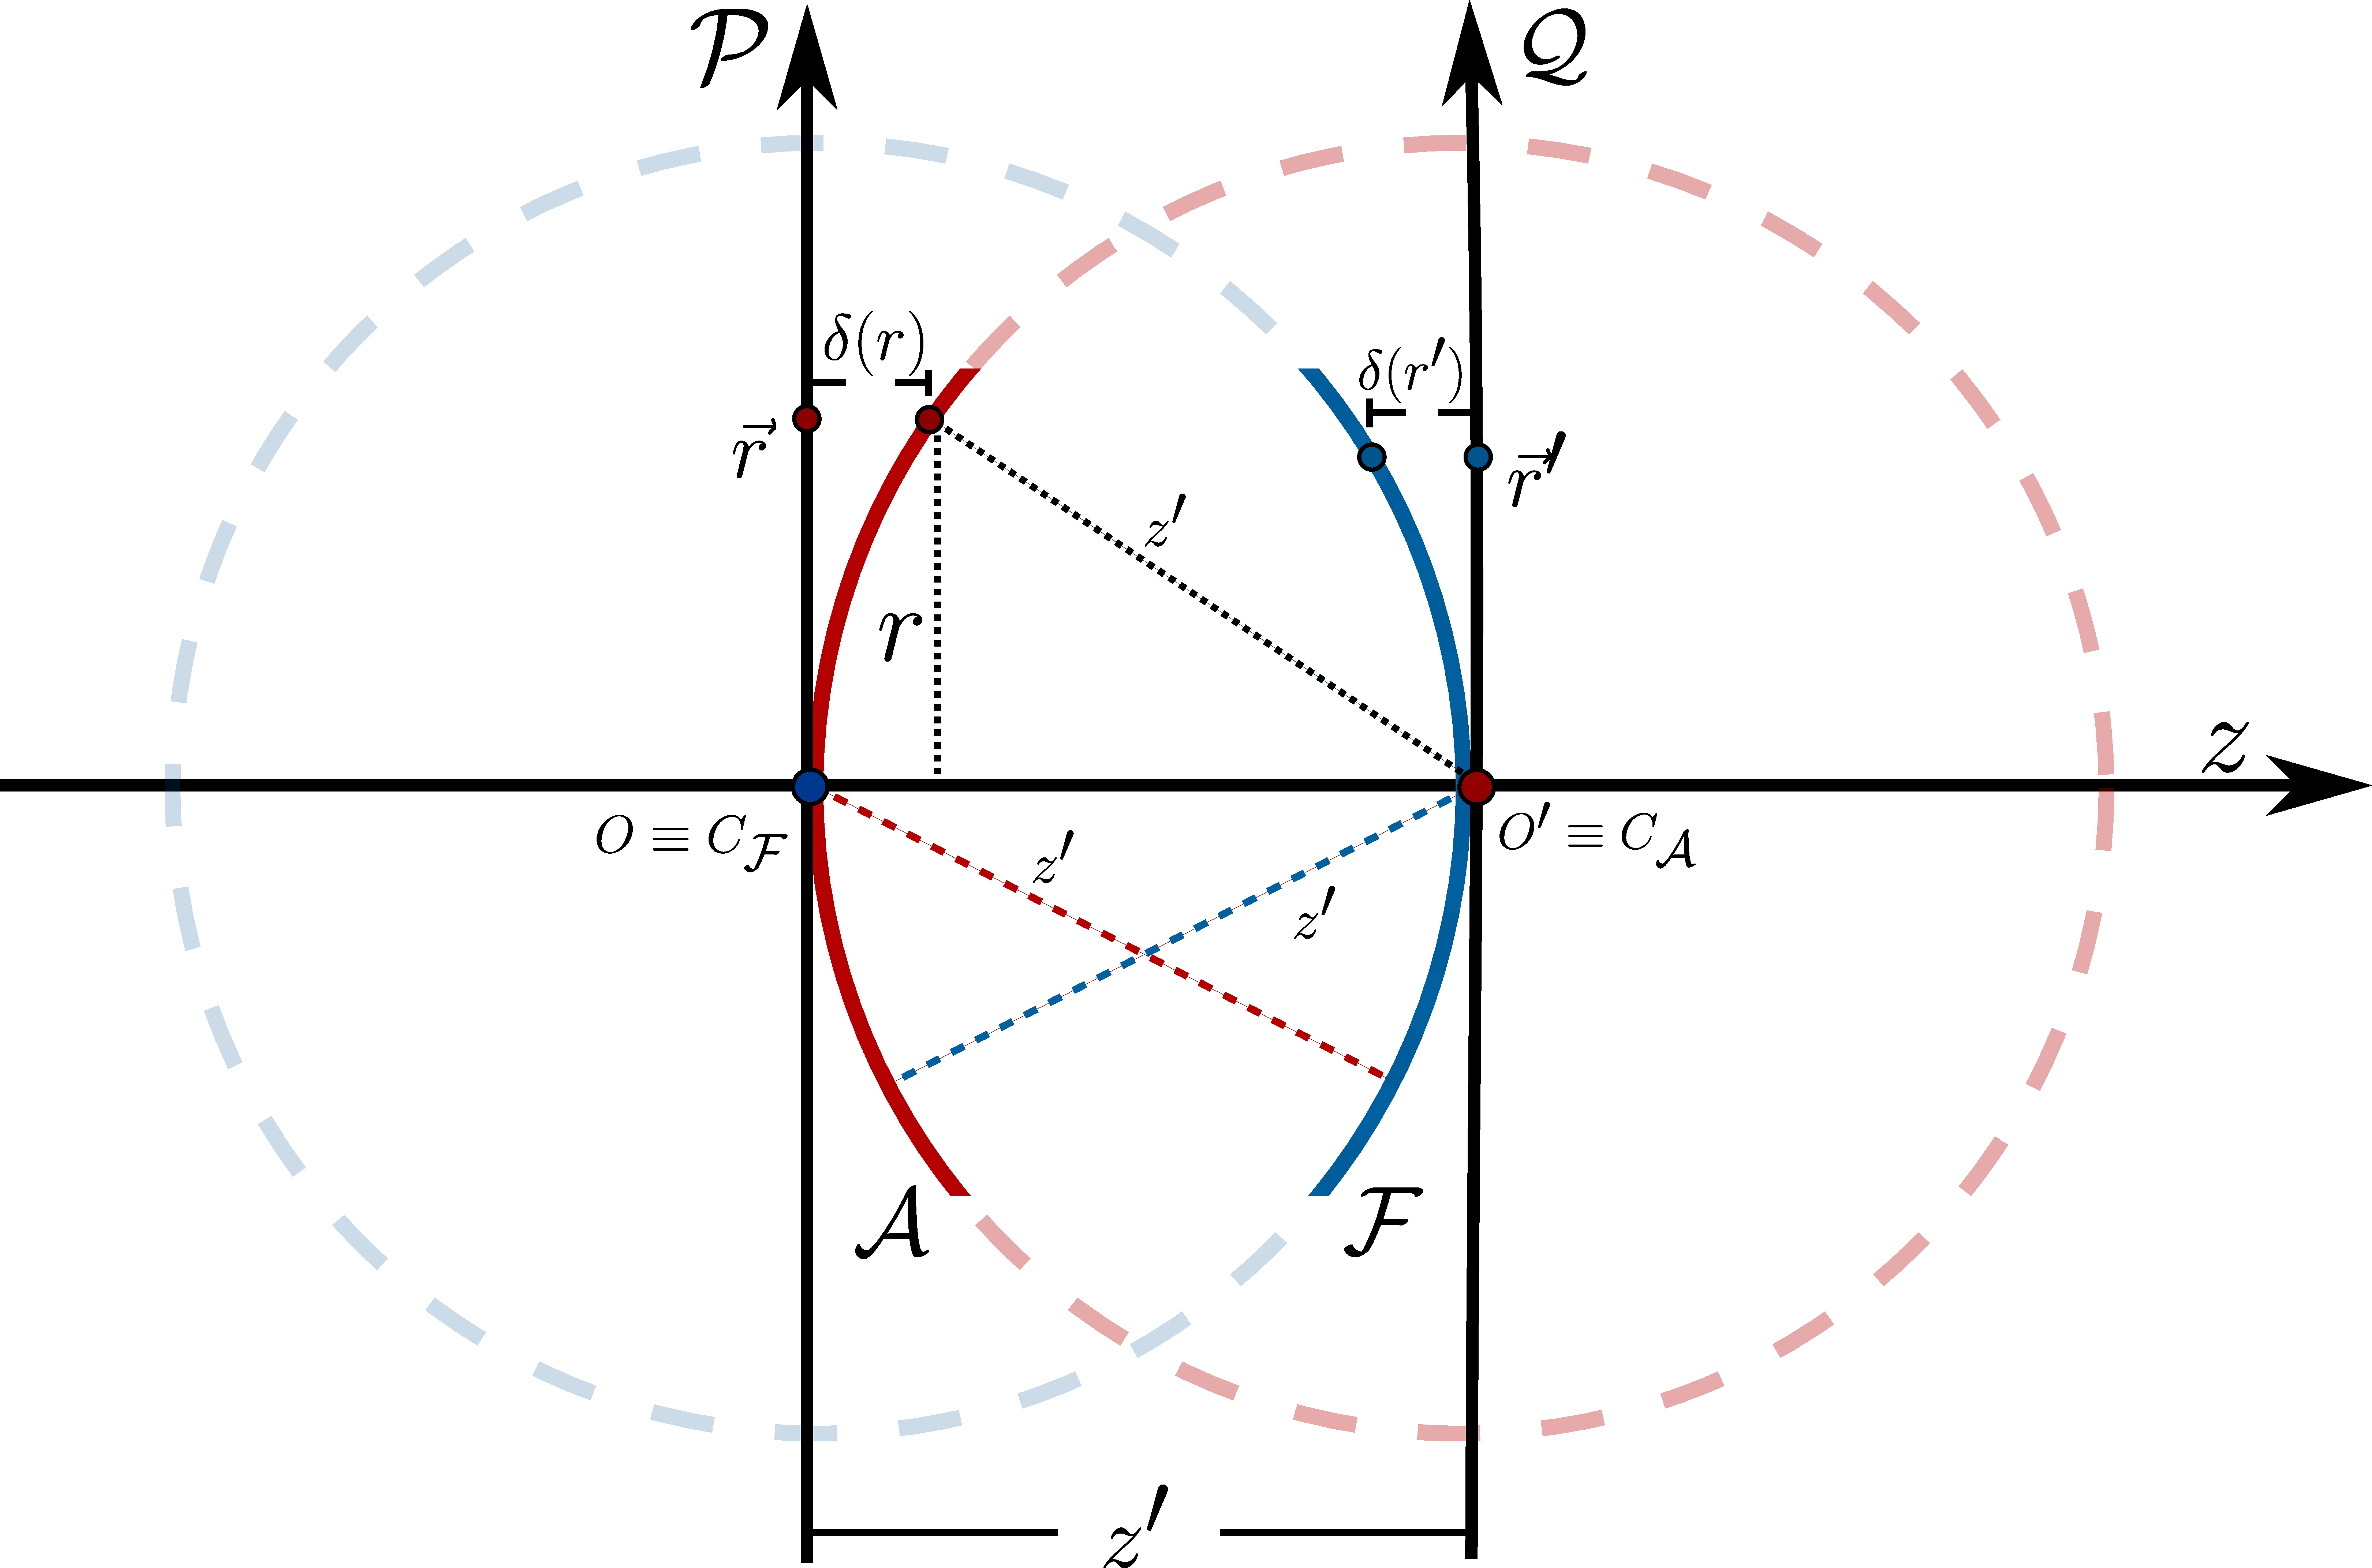
\includegraphics[width=0.7\textwidth]{Capitulo 1/Figuras/ConfocalSpheres.pdf}
			\caption{Geometría de las dos esferas confocales. El casquete $\mathcal{A}$ es tangente
			al plano emisor $\mathcal{P}$ en el vértice $O$ y tiene su centro de curvatura en
			$O'$, mientras que el casquete $\mathcal{F}$ es tangente al plano receptor $\mathcal{Q}$ en
			$O'$ y tiene su centro de curvatura en $O$, de modo que ambos radios son iguales a la distancia de
			propagación $z'$. Leída sobre estas dos superficies, la propagación de Fresnel se reduce a una
			transformación de Fourier exacta, que en el lenguaje de la transformada fraccionaria de Fourier
			de la Sección~\ref{sec:FrFT} corresponde al orden $\alpha = \pi/2$.}
			\label{fig:ConfocalSpheres}
		\end{figure}

		Aplicando \eqref{eq:ConfocalRule} en cada lado con los radios \eqref{eq:ConfocalRadii},
		\begin{equation}\label{eq:ConfocalReferring}
			U(\vec{r}) = u_{\mathcal{A}}(\vec{r})\,e^{-\frac{ik}{2z'}r^{2}}, \qquad
			u_{\mathcal{F}}(\vec{r}\,') = U(\vec{r}\,')\,e^{-\frac{ik}{2z'}r'^{2}} ,
		\end{equation}
		y sustituyendo ambas relaciones en \eqref{eq:FresnelThreeFactors},
		\begin{align*}
			& u_{\mathcal{F}}(\vec{r}\,') = \dfrac{e^{ikz'}}{i\lambda z'}\;
			{\color{red}e^{-\frac{ik}{2z'}r'^{2}}}\;{\color{red}e^{\frac{ik}{2z'}r'^{2}}}
			\int u_{\mathcal{A}}(\vec{r})\;
			{\color{red}e^{-\frac{ik}{2z'}r^{2}}}\;{\color{red}e^{\frac{ik}{2z'}r^{2}}}\;
			e^{-\frac{ik}{z'}\left(xx'+yy'\right)}\,d\sigma ,
		\end{align*}
		donde las cuatro exponenciales en rojo se cancelan en pares, ya que en cada par los dos exponentes son opuestos. Nos queda
		\begin{equation}\label{eq:ConfocalResult}
			\boxed{\;u_{\mathcal{F}}(\vec{r}\,') = \dfrac{e^{ikz'}}{i\lambda z'}\int u_{\mathcal{A}}(\vec{r})\,
			\exp\left[-\dfrac{ik}{z'}\left(xx'+yy'\right)\right]d\sigma ,\;}
		\end{equation}
		que es exactamente la expresión de Fraunhofer \eqref{Fraunhofer} \textit{sin el factor de curvatura}. Esto demuestra la afirmación.

		Son pertinentes tres comentarios, porque el resultado es más fuerte de lo que parece.

		En la derivación de \eqref{Fraunhofer} el factor $e^{ikr^{2}/2z'}$ fue \textit{despreciado} apelando al campo lejano. Aquí no ha sido despreciado, ha sido \textit{absorbido} por la elección de la superficie de referencia, y \eqref{eq:ConfocalResult} es por lo tanto exacta dentro de la aproximación de Fresnel, para cualquier distancia de propagación $z'$. La lección es que la difracción de Fraunhofer no es en realidad un régimen de distancias sino un enunciado sobre geometría: es lo que parece la propagación de Fresnel cuando el campo se lee sobre dos esferas confocales. El factor de curvatura que sobrevive fuera de la integral en \eqref{Fraunhofer} no es sino el precio de insistir en leer el campo sobre un plano, y esta es precisamente la interpretación anticipada en la Figura~\ref{fig:cardinals}.

		Introduciendo la frecuencia espacial asociada al punto de observación,
		\begin{equation}\label{eq:ConfocalFrequency}
			\vec{\nu} = \dfrac{\vec{r}\,'}{\lambda z'}, \qquad \dfrac{k}{z'}\left(xx'+yy'\right) = \dfrac{2\pi}{\lambda z'}\,\vec{r}\cdot\vec{r}\,' = 2\pi\,\vec{r}\cdot\vec{\nu},
		\end{equation}
		la ecuación \eqref{eq:ConfocalResult} se convierte en
		\begin{equation}\label{eq:ConfocalFourier}
			u_{\mathcal{F}}(\lambda z'\,\vec{\nu}) = \dfrac{e^{ikz'}}{i\lambda z'}\,\widehat{u_{\mathcal{A}}}(\vec{\nu}), \qquad \widehat{u_{\mathcal{A}}}(\vec{\nu}) = \int u_{\mathcal{A}}(\vec{r})\,e^{-2\pi i\,\vec{r}\cdot\vec{\nu}}\,d\sigma ,
		\end{equation}
		de modo que la coordenada de observación sobre la esfera $\mathcal{F}$ es, salvo por el factor de escala $\lambda z'$, la frecuencia espacial del campo sobre la esfera $\mathcal{A}$. Este es el sentido preciso en el cual un sistema difractante realiza un análisis de Fourier del objeto, la afirmación a la que Abbe había llegado cualitativamente en 1873 \citep{abbe1873beitrage}.

		Las únicas aproximaciones usadas son las ya contenidas en \eqref{Fresnel} junto con la expansión a primer orden \eqref{eq:ConfocalSagitta} de la sagita, de modo que el resultado se mantiene mientras la región iluminada satisfaga $r_{\max}\ll z'$, que es la condición para que los casquetes no se aparten apreciablemente de sus planos tangentes. Cuando esto deja de cumplirse hay que abandonar la descripción paraxial, tal como se señala al final de la siguiente sección.

		Por último, vale la pena registrar que este ejemplo es la primera instancia de un hecho mucho más general. Nada obliga a que las dos esferas de referencia sean confocales, y si se les da un radio común $R$ distinto de $z'$, los dos factores cuadráticos ya no se cancelan sino que se combinan en un chirp, y la propagación se convierte en una transformada fraccionaria de Fourier de un orden fijado por la razón $z'/R$. El caso confocal aquí tratado es el orden particular $\alpha = \pi/2$. Este es el tema de la Sección~\ref{sec:FrFT}.

\section{La aproximación de Fraunhofer}

Finalmente, a partir de la expresión \eqref{Fresnel} puede llevarse a cabo una segunda aproximación, correspondiente al campo lejano o régimen de Fraunhofer, en el cual las distancias de observación son considerablemente mayores que el área sobre la cual se desea estudiar el campo propagado (ya sea a través de una rendija u otro objeto). Nos concentramos en el factor
\begin{align}
	\exp\left( \frac{ik}{2z'} ((x-x')^2 + (y-y')^2) \right)
	&= \exp\left( \frac{ik}{2z'} (x^2 + y^2) \right)
	\exp\left( \frac{ik}{2z'} (x'^2 + y'^2) \right) \notag \\
	&\quad \times \exp\left( -\frac{ik}{z'} (xx' + yy') \right),
\end{align}
donde la primera de las tres exponenciales es la fase cuadrática acumulada a través de la abertura misma. Fijarla en la unidad es el paso que define el campo lejano, y la condición para hacerlo es que la mayor fase que pueda producir sobre la región iluminada sea pequeña.

\begin{Assumption}
	La fase cuadrática adquirida a través de la abertura es despreciable, $k\,r_{\max}^{2}/2z' \ll 1$, es decir, $z' \gg \pi r_{\max}^{2}/\lambda$, de modo que el número de Fresnel de la abertura es pequeño comparado con la unidad.
\end{Assumption}

Con $\exp\left( \frac{ik}{2z'} (x^2 + y^2) \right) \approx 1$ obtenemos
\begin{equation}
	\label{Fraunhofer}
	U(\vec{r}') = \dfrac{e^{ikz'}}{i\lambda z'} \exp \left(\dfrac{ik}{2z'} (x'^2 + y'^2)\right) \int U(\vec{r}) \exp\left( -\frac{ik}{z'} (xx' + yy') \right) d\sigma .
\end{equation}
Allí todavía podemos apreciar un término de fase cuadrática fuera de la integral, habitualmente llamado factor de curvatura, que muestra precisamente el desfase inducido por la diferencia de camino óptico entre un plano llamado pantalla de observación y una superficie esférica de radio $z'$ (la distancia de propagación del campo a lo largo del eje óptico), conocida como esfera cardinal. La introducción de esta superficie esférica resulta bastante útil cuando se desea describir la difracción de Fraunhofer sobre una pantalla como una propagación de Fresnel a través de dos esferas cardinales confocales, como se muestra en la Figura~\ref{fig:cardinals}.

\begin{figure}[htbp]
	\centering
	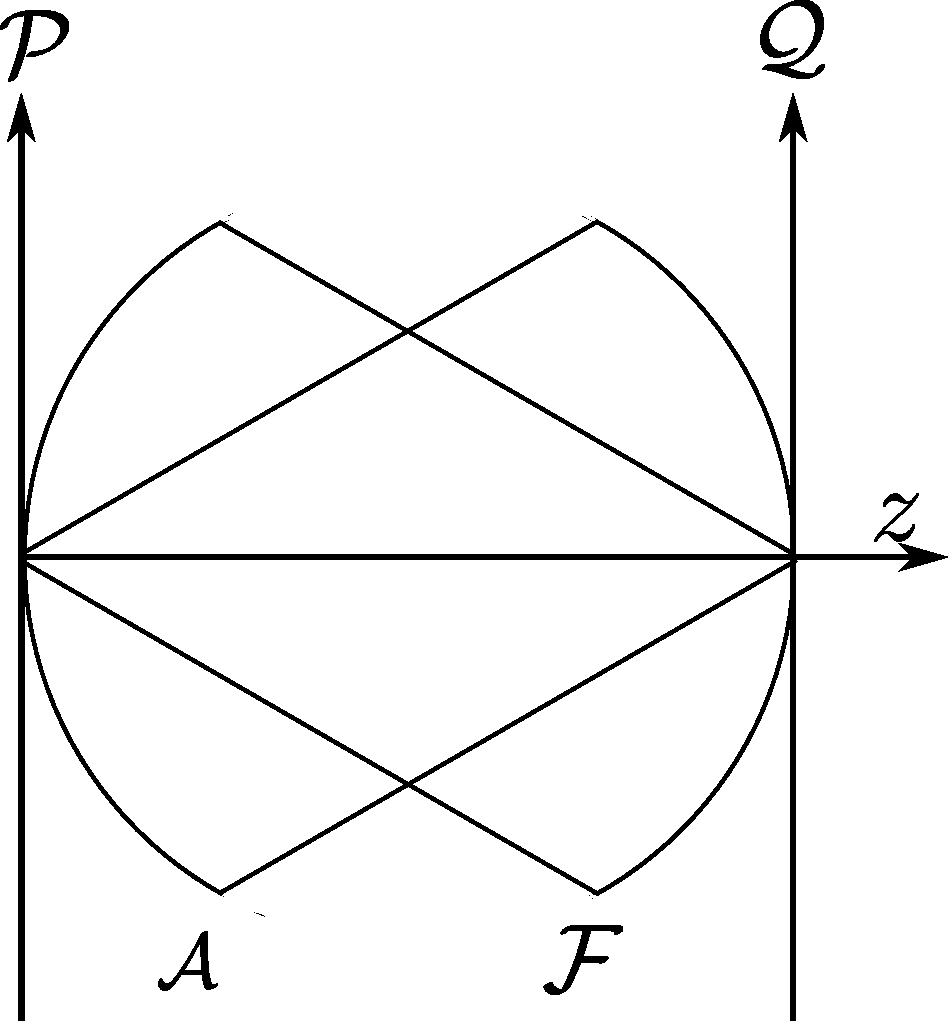
\includegraphics[width=0.5\linewidth]{Capitulo 1/Figuras/Cardinales}
	\caption{Esquema de las esferas cardinales confocales, con radios iguales a la distancia de propagación $z'$ del campo.}
	\label{fig:cardinals}
\end{figure}

Esto cobra más sentido una vez que analizamos el efecto de cada paso de propagación. Resulta claro que, sin imponer aproximaciones de campo lejano desde el inicio, al propagar el campo en $\mathcal{A}$ hacia $\mathcal{F}$ con la aproximación de Fresnel, obtendríamos
\begin{equation}
	U_{\mathcal{F}}(\vec{r}\,') = \dfrac{e^{ikz'}}{i\lambda z'} \exp\left( \frac{ik}{2z'} (x'^2 + y'^2) \right)  \int u_{\mathcal{A}}
	\exp\left( \frac{ik}{2z'} (x^2 + y^2) \right)
	\exp\left( -\frac{ik}{z'} (xx' + yy') \right)d\sigma ,
\end{equation}
donde podemos asociar $u_{\mathcal{A}}$, es decir, el campo sobre la esfera $\mathcal{A}$, con el campo sobre $\mathcal{P}$ multiplicado por su factor cuadrático correspondiente $u_{\mathcal{P}} = u_{\mathcal{A}} (\vec{r}) \exp{\left( \dfrac{ik}{2z'}(x^2+y^2) \right)}$, mientras que el término $\exp{\left( \frac{ik}{2z'} (x'^2 + y'^2) \right)}$ puede entenderse como el factor resultante de pasar el campo de la esfera $\mathcal{F}$ a la pantalla $\mathcal{Q}$, de modo que el campo sobre $\mathcal{F}$ correspondería a
\begin{equation}
	u_{\mathcal{Q}}(\vec{r}\,') = \dfrac{e^{ikz'}}{i\lambda z'} \int u_{\mathcal{P}}
	\exp\left( -\frac{ik}{z'} (xx' + yy') \right)d\sigma ,
\end{equation}
recuperando así una expresión de Fraunhofer para la difracción sobre $\mathcal{Q}$. Cabe señalar que debe verificarse si el estudio del campo propagado es válido dentro de un régimen paraxial, en el que el campo está confinado a la vecindad del eje óptico y por lo tanto la curvatura de la esfera cardinal no difiere mucho del plano (la pantalla). En los casos en que el factor de curvatura deja de ser despreciable, el régimen paraxial pierde validez y el problema debe abordarse desde un punto de vista metaxial.

Vale la pena detenerse aquí a contar, porque este es el lugar en que se cumple la promesa hecha al comienzo del capítulo. Diecisiete supuestos separan las ecuaciones de Maxwell de la integral de Fraunhofer \eqref{Fraunhofer}, y se agrupan en seis familias. Cinco fueron necesarios simplemente para reemplazar el campo electromagnético por una única cantidad escalar: se descartó la interacción magnética, se vació el medio de cargas y corrientes, se congeló la polarización primero en el tiempo y luego en el espacio, y se declaró transversal el campo. Un sexto redujo la luz policromática a una componente espectral a la vez. Cuatro más se gastaron en construir el aparato integral, exigiendo suavidad del campo, vaciando de fuentes la región de observación, reduciendo el emisor elemental a un punto y prohibiendo que llegara radiación alguna desde el infinito. Dos se gastaron en la pantalla, cuyo material fue idealizado hasta desaparecer y sobre la cual el campo fue luego prescrito a mano. Uno colocó al observador a muchas longitudes de onda de la abertura. Tres construyeron el régimen paraxial, truncando la expansión binomial, tratando la amplitud y la fase con distintos grados de precisión y enderezando a la unidad el factor de oblicuidad. El decimoséptimo y último empujó al observador hacia el campo lejano.

De este recuento se siguen dos lecciones. La primera es que la elegancia de \eqref{Fraunhofer}, una simple transformada de Fourier de la abertura, se compra en lugar de regalarse: cada uno de los diecisiete pasos ha estrechado la clase de experimentos que la fórmula puede describir, y cada uno de ellos puede violarse en un laboratorio. La teoría escalar falla cuando la abertura se vuelve comparable con la longitud de onda, cuando la apertura numérica es grande, cuando la pantalla es un buen conductor y la polarización de la iluminación resulta importar, o cuando la distancia de observación no es suficientemente grande para que el número de Fresnel sea pequeño; en cada uno de esos casos el culpable puede rastrearse hasta un elemento definido de la lista anterior. La segunda lección es la más notable, y es la razón por la que la teoría se enseña en absoluto: la fórmula funciona de todos modos, y funciona en un rango de situaciones mucho más amplio de lo que los supuestos tendrían derecho a garantizar. Entender cuál de los diecisiete está a punto de romperse es, en la práctica, todo el arte de aplicar la teoría de la difracción.


Estudiar la propagación del campo mediante la difracción de Fresnel es de gran importancia porque, como se discutirá más adelante, guarda una estrecha relación con lo que se conoce como la transformada fraccionaria de Fourier, una herramienta que surge naturalmente al encadenar pasos de propagación paraxial.

\section{La transformada fraccionaria de Fourier}\label{sec:FrFT}

	La sección anterior cerró con la observación de que la propagación de Fresnel guarda una estrecha relación con la transformada fraccionaria de Fourier. Esa observación es el tema de la presente sección, y merece un tratamiento cuidadoso por dos razones. La primera es que la transformada fraccionaria de Fourier no es una curiosidad formal sino el lenguaje natural en el que debería escribirse la propagación paraxial, en el mismo sentido en que la transformada de Fourier ordinaria es el lenguaje natural del campo lejano. La segunda es que el objeto en sí, una familia continua de operadores que interpola entre la identidad y la transformación de Fourier, tiene una historia larga e instructiva, en la que la misma idea fue redescubierta de manera independiente en el análisis puro, en la mecánica cuántica, en el procesamiento de señales y en la óptica, antes de que alguien se percatara de que las cuatro comunidades hablaban del mismo grupo uniparamétrico.

	Una palabra sobre notación antes de comenzar. En \eqref{Fresnel} la distancia de propagación aparecía como $z'$, la coordenada axial del punto de observación, quedando la abertura fija en el origen del eje. En la presente sección las dos superficies de referencia se tratan en pie de igualdad y ninguna de ellas está privilegiada, de modo que colocamos la superficie emisora en el origen y escribimos simplemente $z$ para la distancia a la receptora. La $z$ de esta sección es, por lo tanto, la $z'$ de \eqref{Fresnel}, y ninguna coordenada axial de la variable de integración aparece en ningún lugar de lo que sigue.


	\subsection{Contexto histórico del análisis de Fourier y de sus potencias fraccionarias}

		La historia comienza, como tantas historias de la física matemática, con una cuerda vibrante. En 1747 Jean le Rond d'Alembert escribió la ecuación de onda de una cuerda tensa y la resolvió superponiendo dos ondas viajeras \citep{dalembert1747recherches}, solución que Leonhard Euler generalizó de inmediato a formas iniciales arbitrarias \citep{euler1748vibration}. Seis años más tarde Daniel Bernoulli propuso algo que a sus contemporáneos les pareció físicamente obvio y matemáticamente escandaloso a la vez, a saber, que todo movimiento posible de la cuerda podía escribirse como una suma de los modos sinusoidales de vibración \citep{bernoulli1753reflexions}. Euler y d'Alembert rechazaron ambos la afirmación. Su objeción no era estética sino lógica, ya que una suma de senos es un objeto suave y periódico mientras que la forma inicial de una cuerda pulsada tiene un pico, y ningún matemático del siglo XVIII estaba dispuesto a aceptar que una suma infinita de funciones analíticas pudiera reproducir una curva con un quiebre. La disputa duró medio siglo y nunca fue zanjada por quienes la iniciaron.

		Quedó zanjada, en cierto sentido, por alguien que no intentaba zanjarla. En 1807 Joseph Fourier presentó al Institut de France una memoria sobre la propagación del calor en los sólidos en la que afirmaba, y usaba, precisamente la representación que Euler había rechazado. Los árbitros, entre ellos Lagrange, rechazaron la memoria. Lagrange en particular nunca aceptó la generalidad de la expansión trigonométrica, y Fourier tuvo que esperar hasta 1822 para publicar la versión madura de sus ideas como la \textit{Théorie Analytique de la Chaleur} \citep{fourier1822theorie}. Lo que Fourier había entendido, y sus árbitros no, es que la pregunta de si la serie converge a la función es una pregunta distinta de si la serie es útil, y que los coeficientes pueden calcularse mediante una integral sin importar la posición filosófica de cada quien sobre la convergencia. El paso de la serie sobre un intervalo finito a la integral sobre toda la recta, que es lo que hoy llamamos la transformación de Fourier, ya está presente en ese libro como un caso límite.

		La osadía de Fourier dejó una deuda que el siglo XIX pasó décadas pagando. Peter Gustav Lejeune Dirichlet dio en 1829 el primer teorema de convergencia genuino, mostrando que la serie de una función monótona a trozos con un número finito de discontinuidades converge al promedio de los límites laterales \citep{dirichlet1829convergence}. Bernhard Riemann, en su habilitación de 1854 publicada póstumamente en 1867, planteó la pregunta inversa de qué funciones admiten en absoluto una representación trigonométrica, y al hacerlo se vio obligado a inventar una teoría de la integración \citep{riemann1867darstellbarkeit}. Georg Cantor, estudiando la unicidad de las representaciones trigonométricas, fue llevado a clasificar los conjuntos excepcionales sobre los cuales dos series distintas pueden coincidir, y de esa clasificación creció la propia teoría de conjuntos \citep{cantor1872ausdehnung}. Henri Lebesgue construyó una nueva integral en parte para hacer que la teoría de las series trigonométricas se comportara \citep{lebesgue1903series}. No es exagerado decir que buena parte del análisis moderno existe porque Fourier escribió una fórmula que nadie podía justificar.

		La teoría alcanzó su forma definitiva en el siglo XX. Michel Plancherel demostró en 1910 la identidad que lleva su nombre, estableciendo que la transformación de Fourier es una isometría del espacio de funciones de cuadrado integrable sobre sí mismo \citep{plancherel1910contribution}. Este es, para nuestros propósitos, el hecho estructural más importante sobre la transformación, porque una isometría de un espacio de Hilbert sobre sí mismo es un operador unitario, y los operadores unitarios son exactamente los objetos que pueden elevarse a potencias continuas. Norbert Wiener \citeyearpar{wiener1933fourier} y Edward Titchmarsh \citeyearpar{titchmarsh1937introduction} consolidaron la teoría analítica en los dos tratados que definieron el tema durante una generación, y en 1965 James Cooley y John Tukey redescubrieron un algoritmo que redujo el costo numérico de la transformación discreta de una ley cuadrática a una logarítmica, y con ello llevó el análisis de Fourier del pizarrón a todos los instrumentos de laboratorio \citep{cooley1965algorithm}.

		La óptica entró en la historia por una puerta distinta. Ernst Abbe ya había entendido en 1873, tratando de explicar por qué sus microscopios no podían resolver detalles arbitrariamente finos, que el objetivo de un microscopio realiza una descomposición del objeto en frecuencias espaciales y que la abertura del instrumento trunca esa descomposición \citep{abbe1873beitrage}. La idea permaneció esencialmente cualitativa hasta que Pierre-Michel Duffieux publicó en 1946 el primer tratado sistemático sobre la integral de Fourier en óptica \citep{duffieux1946integrale}, antecesor directo del tratamiento moderno que se encuentra en Goodman \citeyearpar{goodman2005introduction}. Hacia mediados del siglo XX era un lugar común que el campo lejano de una abertura es la transformada de Fourier de la abertura, que es la afirmación que dedujimos en la sección sobre la aproximación de Fraunhofer.

		La idea de una potencia \textit{fraccionaria} de la transformación de Fourier tiene una genealogía separada y mucho menos lineal. Su semilla es una observación puramente analítica. Charles Hermite había introducido en 1864 los polinomios que llevan su nombre \citep{hermite1864nouveau}, y Ferdinand Gustav Mehler había hallado en 1866 la función generadora bilineal de esos polinomios \citep{mehler1866entwicklung}, fórmula que hará todo el trabajo por nosotros más adelante en esta sección. En 1929 Norbert Wiener publicó una breve nota en la que observaba que las funciones de Hermite son funciones propias de la transformación de Fourier con valores propios que son las cuatro raíces cuartas de la unidad \citep{wiener1929hermitian}. La observación es elemental una vez enunciada, pero es toda la idea, porque un operador cuyo espectro se conoce puede elevarse a cualquier potencia que se desee simplemente elevando los valores propios a esa potencia.

		Edward Uhler Condon dio ese paso explícitamente en 1937, en un artículo cuyo título dice exactamente lo que hace, a saber, sumergir la transformación de Fourier en un grupo continuo de transformaciones funcionales \citep{condon1937immersion}. Condon estaba interesado en la estructura teórico-grupal y en la conexión con el oscilador armónico cuántico, y ya notó que el generador de la familia continua es el hamiltoniano del oscilador. Dos años más tarde Hermann Kober, trabajando desde el punto de vista de las transformaciones integrales, construyó raíces de las transformaciones de Fourier y de Hankel y dio los núcleos correspondientes \citep{kober1939wurzeln}. Valentine Bargmann llegó a la misma familia en 1961 desde otra dirección distinta, a través de su espacio de Hilbert de funciones enteras, donde las potencias fraccionarias actúan como simples rotaciones de la variable compleja \citep{bargmann1961hilbert}. Nicolaas de Bruijn las recuperó una vez más en 1973 en su teoría de funciones generalizadas construida sobre la distribución de Wigner \citep{debruijn1973theory}. Cada uno de estos autores tuvo el objeto entre las manos y ninguno le dio un nombre que perdurara.

		El nombre y el tratamiento sistemático se deben a Victor Namias, quien en 1980 publicó el artículo que la comunidad óptica toma hoy como el origen del tema \citep{namias1980fractional}. La contribución de Namias no fue meramente terminológica. Definió la transformación de orden fraccionario de dos maneras equivalentes, como un operador diferencial obtenido al exponenciar el hamiltoniano del oscilador armónico y como un operador integral con núcleo explícito, mostró que las dos definiciones coinciden, y luego usó la herramienta resultante para resolver problemas concretos de mecánica cuántica que resultan incómodos en el lenguaje de Fourier ordinario. Es su derivación la que reproduciremos por completo en la siguiente subsección.

		El tratamiento de Namias fue, según sus propios estándares, el de un físico en ejercicio. La integral que escribió no converge absolutamente para toda función que uno quisiera transformar, la raíz cuadrada que aparece en la constante de normalización se escribe sin especificar qué rama se entiende, y la aditividad de los órdenes se verifica sobre la expansión en funciones propias en lugar de demostrarse en un dominio bien definido. Estas no son objeciones pedantes, porque una elección descuidada de rama hace que la ley de composición falle por un signo. Adam McBride y Fiona Kerr repararon todo esto en 1987 \citep{mcbride1987namias}, dando una definición que converge absolutamente en el espacio de Schwartz, fijando la rama de manera que la ley de composición se cumpla para todos los órdenes reales, y demostrando que la familia resultante es un genuino grupo continuo uniparamétrico. Kerr extendió poco después la construcción a espacios de funciones generalizadas \citep{kerr1988distributional} y al espacio de funciones de cuadrado integrable con aplicaciones a ecuaciones diferenciales \citep{kerr1988namias}.

		Mientras los analistas ordenaban la teoría, la comunidad óptica redescubrió el objeto experimentalmente. En 1993 David Mendlovic y Haldun Ozaktas publicaron un par de artículos mostrando que un medio de índice gradual de la longitud apropiada realiza una transformación fraccionaria de Fourier sobre el campo que lo atraviesa \citep{mendlovic1993fractional, ozaktas1993fractional}, y Adolf Lohmann mostró ese mismo año que el orden fraccionario no es otra cosa que un ángulo de rotación de la distribución de Wigner del campo, lo cual dio a toda la construcción un significado transparente en el espacio de fase y una implementación inmediata en óptica de volumen con dos lentes \citep{lohmann1993image}. Un año después Pierre Pellat-Finet demostró el resultado que más directamente nos concierne, a saber, que la difracción de Fresnel entre dos casquetes esféricos es exactamente una transformación fraccionaria de Fourier, con un orden fijado por la geometría \citep{pellatfinet1994fresnel}, resultado desarrollado extensamente junto con Georges Bonnet \citep{pellatfinet1994fractional} e incorporado más tarde a un tratado completo sobre óptica metaxial y fraccionaria de Fourier \citep{pellatfinet2009optique}. Paralelamente, Luís Almeida introdujo la transformación en el procesamiento de señales como una interpolación entre las representaciones temporal y frecuencial \citep{almeida1994fractional}, y todo el cuerpo de aplicaciones ópticas fue recopilado por Ozaktas, Zalevsky y Kutay \citeyearpar{ozaktas2001fractional}.

		Vale la pena detenerse en el hecho de que la literatura no usa una única noción de orden fraccionario, y un lector que se mueva entre artículos encontrará al menos cinco convenciones. La primera es la introducida por Namias, en la que el orden es un ángulo $\alpha$ medido en radianes, correspondiendo la transformación de Fourier ordinaria a $\alpha = \pi/2$ y la identidad a $\alpha = 0$. La segunda, estándar en el procesamiento de señales tras Ozaktas, Mendlovic y Lohmann, reemplaza el ángulo por un orden adimensional $a$ definido mediante $\alpha = a\pi/2$, de modo que la transformación ordinaria es la transformación de orden uno y el operador de paridad es la transformación de orden dos. La tercera es el orden óptico usado por Pellat-Finet, que de nuevo es un ángulo pero está ligado a un par de esferas de referencia en lugar de a una asignación abstracta de valores propios, y que por lo tanto depende de la geometría elegida para describir la propagación. La cuarta es el orden complejo, introducido por Chung-Chieh Shih \citeyearpar{shih1995optical} y realizado ópticamente por Luís Bernardo y Olívio Soares \citeyearpar{bernardo1996optical}, en la cual se permite que el parámetro abandone el eje real y la transformación adquiere una ponderación gaussiana además de su chirp. La quinta no es una convención sino una ambigüedad genuina, y merece énfasis. Puesto que la transformación de Fourier ordinaria satisface $\mathcal{F}^{4} = \mathcal{I}$, el problema de definir $\mathcal{F}^{a}$ es el problema de elegir de manera continua una raíz cuarta de la identidad, y esa elección no es única. Namias asigna a la función propia de índice $n$ el valor propio $e^{-in\alpha}$, que es la elección que hace del generador el hamiltoniano del oscilador armónico, pero Shih mostró que una asignación distinta y perfectamente consistente, basada en ponderar las cuatro potencias de $\mathcal{F}$, produce una familia inequivalente \citep{shih1995fractionalization}. Gianfranco Cariolaro y colaboradores clasificaron después todas las fraccionalizaciones admisibles en un único marco \citep{cariolaro1998unified}, y Çağatay Candan, Alper Kutay y Ozaktas resolvieron el problema discreto correspondiente \citep{candan2000discrete}. Cuando un artículo habla de \textit{la} transformada fraccionaria de Fourier sin mayor calificación, casi siempre se refiere a la familia de Namias, y es esa la que construiremos.

		Por último, cabe decir que la transformación fraccionaria de Fourier no es un objeto aislado sino el miembro no trivial más simple de una familia mucho más amplia. Marcos Moshinsky y Christiane Quesne introdujeron en 1971 las transformaciones canónicas lineales, las representaciones unitarias del grupo de transformaciones lineales del espacio de fase que preservan la forma simpléctica \citep{moshinsky1971linear}, y Kurt Bernardo Wolf desarrolló su teoría como transformaciones integrales \citep{wolf1979integral}. Stuart Collins había escrito en 1970 la integral de difracción de un sistema paraxial arbitrario en términos de la matriz de ese sistema \citep{collins1970lens}, que es la misma familia vista desde el lado de la ingeniería. En ese lenguaje, las transformaciones fraccionarias de Fourier son exactamente los elementos elípticos del grupo, es decir, las rotaciones del espacio de fase, mientras que la propagación libre sobre un plano y la acción de una lente delgada son elementos parabólicos y las magnificaciones son elementos hiperbólicos. La razón por la que la transformación fraccionaria de Fourier ocupa un lugar tan privilegiado en óptica es que, como demostraremos, una vez que el campo se refiere al par correcto de superficies esféricas, la propagación libre se convierte en una rotación pura.

	\subsection{La transformada fraccionaria de Fourier como operador diferencial e integral}

		A lo largo de esta subsección trabajamos en una sola variable transversal, ya que el caso bidimensional se sigue tomando el producto tensorial de dos transformaciones unidimensionales idénticas, y adoptamos la convención simétrica
		\begin{equation}\label{eq:FrFT:FT}
			\mathcal{F}[f](x) = \frac{1}{\sqrt{2\pi}}\int_{-\infty}^{\infty} f(y)\,e^{-ixy}\,\mathrm{d}y,
		\end{equation}
		que es la convención que hace a $\mathcal{F}$ unitaria sobre $L^2(\mathbb{R})$ por el teorema de Plancherel \citeyearpar{plancherel1910contribution}, y que concuerda con el signo del núcleo que apareció en la integral de Fraunhofer \eqref{Fraunhofer}. Aplicando \eqref{eq:FrFT:FT} dos veces se obtiene el operador de paridad, y cuatro veces la identidad,
		\begin{equation}\label{eq:FrFT:Powers}
			\mathcal{F}^{2} = \mathcal{P}, \qquad \mathcal{P}f(x) = f(-x), \qquad \mathcal{F}^{4} = \mathcal{I},
		\end{equation}
		de modo que las potencias enteras de $\mathcal{F}$ forman un grupo cíclico de orden cuatro. Todo el contenido de esta subsección es la construcción de un grupo continuo en el cual ese grupo cíclico de cuatro elementos se aloja como subgrupo.

		Antes de comenzar, es necesario fijar un punto de vocabulario, porque las dos palabras involucradas se confunden rutinariamente y la distinción es esencial para todo lo que sigue.

		\begin{myDef}
			\textit{(Transformación y transformada)} Una \textit{transformación} es un operador, es decir, una aplicación $\mathcal{F}_{\alpha} : \mathcal{H} \to \mathcal{H}$ de un espacio de funciones en sí mismo. Una \textit{transformada} es la imagen de un elemento particular bajo esa aplicación, es decir, la función $\mathcal{F}_{\alpha}f$ obtenida al aplicar la transformación a una $f$ dada.
		\end{myDef}

		La distinción no es pedante. Todo lo que hace valiosa a la construcción fraccionaria de Fourier es un enunciado sobre \textit{transformaciones} y no sobre transformadas: la familia $\{\mathcal{F}_{\alpha}\}_{\alpha\in\mathbb{R}}$ es un grupo uniparamétrico, su ley de composición es $\mathcal{F}_{\alpha}\mathcal{F}_{\beta} = \mathcal{F}_{\alpha+\beta}$, su generador es el hamiltoniano del oscilador armónico, y sus elementos son unitarios. Ninguna de estas frases puede siquiera formularse al nivel de una única transformada, porque una transformada es simplemente una función y no lleva estructura de grupo alguna. En la aplicación óptica de la subsección anterior, el punto se vuelve físico en lugar de lingüístico: es la propagación del campo a lo largo de una distancia lo que es una transformación, mientras que el campo observado sobre la superficie receptora es una transformada, y la razón por la cual la propagación se compone de manera tan simple es una propiedad de los operadores, no de ningún campo en particular.

		\subsubsection{Las funciones propias de la transformación de Fourier}

			La construcción descansa sobre un único hecho, observado por Wiener en 1929 \citep{wiener1929hermitian}, a saber, que la transformación de Fourier posee un conjunto ortonormal completo de funciones propias construidas a partir de los polinomios de Hermite \citep{hermite1864nouveau}. Deduzcámoslo, ya que cada paso posterior depende del valor preciso de los valores propios. Recordemos la función generadora de los polinomios de Hermite,
			\begin{equation}\label{eq:FrFT:HermiteGen}
				e^{2xt-t^{2}} = \sum_{n=0}^{\infty}\frac{H_{n}(x)}{n!}t^{n},
			\end{equation}
			y definamos la función generadora de las funciones de Hermite multiplicando \eqref{eq:FrFT:HermiteGen} por la gaussiana $e^{-x^{2}/2}$,
			\begin{equation}\label{eq:FrFT:GDef}
				G(x,t) = e^{-x^{2}/2}\,e^{2xt-t^{2}} = e^{-x^{2}/2}\sum_{n=0}^{\infty}\frac{H_{n}(x)}{n!}t^{n}.
			\end{equation}
			Transformamos ahora \eqref{eq:FrFT:GDef} respecto a $x$. Escribiendo el exponente completo del integrando de \eqref{eq:FrFT:FT},
			\begin{align*}
				& -\frac{x^{2}}{2} + 2xt - t^{2} - i\xi x = -\frac{x^{2}}{2} + x\left(2t-i\xi\right) - t^{2} = \\
				& -\frac{1}{2}\left[x^{2} - 2x\left(2t-i\xi\right) + {\color{blue}\left(2t-i\xi\right)^{2}}\right] + {\color{blue}\frac{\left(2t-i\xi\right)^{2}}{2}} - t^{2},
			\end{align*}
			donde los dos términos en azul se han sumado y restado, lo cual es lícito porque su suma es cero, y lo cual convierte el primer corchete en un cuadrado perfecto,
			\begin{equation*}
				= -\frac{1}{2}\left[x - \left(2t-i\xi\right)\right]^{2} + \frac{\left(2t-i\xi\right)^{2}}{2} - t^{2}.
			\end{equation*}
			La integral restante es la gaussiana $\int_{-\infty}^{\infty}e^{-\frac{1}{2}(x-a)^{2}}\mathrm{d}x = \sqrt{2\pi}$, válida para $a$ compleja mediante una traslación del contorno de integración, de modo que el factor $1/\sqrt{2\pi}$ de \eqref{eq:FrFT:FT} se cancela exactamente y
			\begin{equation}\label{eq:FrFT:GTransformed}
				\mathcal{F}\left[G(\cdot,t)\right](\xi) = \exp\left[\frac{\left(2t-i\xi\right)^{2}}{2} - t^{2}\right].
			\end{equation}
			Resta reconocer el lado derecho. Expandiendo el cuadrado,
			\begin{align*}
				& \frac{4t^{2} - 4it\xi - \xi^{2}}{2} - t^{2} = 2t^{2} - 2it\xi - \frac{\xi^{2}}{2} - t^{2} = -\frac{\xi^{2}}{2} - 2i\xi t + t^{2} = \\
				& -\frac{\xi^{2}}{2} + 2\xi\left(-it\right) - \left(-it\right)^{2},
			\end{align*}
			puesto que $-(-it)^{2} = +t^{2}$, y comparando con la definición \eqref{eq:FrFT:GDef} concluimos que
			\begin{equation}\label{eq:FrFT:GSelf}
				\mathcal{F}\left[G(\cdot,t)\right](\xi) = G(\xi,-it).
			\end{equation}
			\textit{La función generadora se aplica sobre sí misma con el parámetro rotado un cuarto de vuelta en el plano complejo.} Expandiendo ambos lados de \eqref{eq:FrFT:GSelf} en potencias de $t$ mediante \eqref{eq:FrFT:GDef},
			\begin{equation*}
				\sum_{n=0}^{\infty}\frac{t^{n}}{n!}\,\mathcal{F}\!\left[H_{n}\,e^{-x^{2}/2}\right](\xi) = \sum_{n=0}^{\infty}\frac{\left(-it\right)^{n}}{n!}H_{n}(\xi)e^{-\xi^{2}/2},
			\end{equation*}
			e identificando los coeficientes de $t^{n}$, lo cual es lícito porque ambas series convergen para todo $t$ en una vecindad del origen, obtenemos el resultado buscado. Introduciendo las funciones de Hermite normalizadas
			\begin{equation}\label{eq:FrFT:HermiteFunctions}
				\psi_{n}(x) = \left(2^{n}n!\sqrt{\pi}\right)^{-1/2}H_{n}(x)\,e^{-x^{2}/2}, \qquad \int_{-\infty}^{\infty}\psi_{n}(x)\psi_{m}(x)\,\mathrm{d}x = \delta_{nm},
			\end{equation}
			que forman una base ortonormal completa de $L^{2}(\mathbb{R})$, la relación de valores propios se lee
			\begin{equation}\label{eq:FrFT:Eigen}
				\mathcal{F}\left[\psi_{n}\right] = \left(-i\right)^{n}\psi_{n} = e^{-in\pi/2}\,\psi_{n}.
			\end{equation}

			La ecuación \eqref{eq:FrFT:Eigen} contiene toda la idea. Los valores propios de la transformación de Fourier son $e^{-in\pi/2}$, y el número $\pi/2$ aparece allí no por ninguna propiedad profunda de la exponencial, sino simplemente porque $\mathcal{F}$ es la raíz cuarta de la identidad. Nada nos impide reemplazar $\pi/2$ por un ángulo arbitrario.

		\subsubsection{La definición de Namias y el operador diferencial}

			Siguiendo a Namias \citeyearpar{namias1980fractional}, definimos la transformación fraccionaria de Fourier de orden $\alpha$ prescribiendo su acción sobre la base \eqref{eq:FrFT:HermiteFunctions},
			\begin{equation}\label{eq:FrFT:SpectralDef}
				\mathcal{F}_{\alpha}\left[\psi_{n}\right] = e^{-in\alpha}\,\psi_{n},
			\end{equation}
			y extendiéndola a una $f\in L^{2}(\mathbb{R})$ arbitraria por linealidad y continuidad. Escribiendo la expansión de $f$ en la base,
			\begin{equation}\label{eq:FrFT:Expansion}
				f(x) = \sum_{n=0}^{\infty}c_{n}\psi_{n}(x), \qquad c_{n} = \int_{-\infty}^{\infty}f(y)\psi_{n}(y)\,\mathrm{d}y,
			\end{equation}
			la transformada de orden $\alpha$ es por definición
			\begin{equation}\label{eq:FrFT:SpectralTransform}
				F_{\alpha}(x) \equiv \mathcal{F}_{\alpha}\left[f\right](x) = \sum_{n=0}^{\infty}c_{n}e^{-in\alpha}\psi_{n}(x).
			\end{equation}
			La definición es manifiestamente consistente, ya que $\alpha = 0$ da $F_{0} = f$ por completitud, $\alpha = \pi/2$ reproduce \eqref{eq:FrFT:Eigen}, $\alpha = \pi$ da $\sum c_{n}(-1)^{n}\psi_{n}$, que es el operador de paridad porque $\psi_{n}$ tiene la paridad de $n$, y $\alpha = 2\pi$ devuelve la identidad. La familia es por lo tanto $2\pi$-periódica en $\alpha$ y unitaria, ya que multiplica los coeficientes de una expansión ortonormal por números unimodulares.

			La primera observación de Namias es que \eqref{eq:FrFT:SpectralTransform} puede liberarse de la base y escribirse como un operador diferencial. Derivando \eqref{eq:FrFT:SpectralTransform} respecto al orden,
			\begin{equation}\label{eq:FrFT:dFdalpha}
				\frac{\partial F_{\alpha}}{\partial \alpha}(x) = -i\sum_{n=0}^{\infty}n\,c_{n}e^{-in\alpha}\psi_{n}(x),
			\end{equation}
			nos queda el índice $n$ dentro de la suma, lo cual es inconveniente porque $n$ no es un operador que actúe sobre $x$. El remedio es la ecuación diferencial de las funciones de Hermite. Sustituyendo \eqref{eq:FrFT:HermiteFunctions} en la ecuación de Hermite $H_{n}'' - 2xH_{n}' + 2nH_{n} = 0$ se obtiene, tras el cálculo elemental de las dos derivadas del factor gaussiano,
			\begin{equation}\label{eq:FrFT:HermiteODE}
				\psi_{n}''(x) + \left(2n+1-x^{2}\right)\psi_{n}(x) = 0,
			\end{equation}
			que es precisamente la ecuación de Schrödinger estacionaria del oscilador armónico cuántico en unidades naturales. Resolviendo \eqref{eq:FrFT:HermiteODE} para el índice,
			\begin{equation}\label{eq:FrFT:nPsi}
				n\,\psi_{n}(x) = \frac{1}{2}\left[x^{2}\psi_{n}(x) - \psi_{n}''(x) - \psi_{n}(x)\right],
			\end{equation}
			e insertando \eqref{eq:FrFT:nPsi} en \eqref{eq:FrFT:dFdalpha},
			\begin{align*}
				& \frac{\partial F_{\alpha}}{\partial \alpha}(x) = -\frac{i}{2}\sum_{n=0}^{\infty}c_{n}e^{-in\alpha}\left[x^{2}\psi_{n}(x) - \psi_{n}''(x) - \psi_{n}(x)\right] = \\
				& -\frac{i}{2}\left[x^{2}\sum_{n}c_{n}e^{-in\alpha}\psi_{n}(x) - \frac{\partial^{2}}{\partial x^{2}}\sum_{n}c_{n}e^{-in\alpha}\psi_{n}(x) - \sum_{n}c_{n}e^{-in\alpha}\psi_{n}(x)\right],
			\end{align*}
			donde el índice $n$ ha desaparecido por completo y cada una de las tres sumas es de nuevo $F_{\alpha}$ por \eqref{eq:FrFT:SpectralTransform}. Llegamos así a la formulación diferencial de la transformación fraccionaria de Fourier,
			\begin{equation}\label{eq:FrFT:PDE}
				i\,\frac{\partial F_{\alpha}}{\partial \alpha} = \frac{1}{2}\left[-\frac{\partial^{2}}{\partial x^{2}} + x^{2} - 1\right]F_{\alpha}, \qquad F_{\alpha}\big|_{\alpha=0} = f.
			\end{equation}

			\textbf{\textit{La ecuación \eqref{eq:FrFT:PDE} es la definición de Namias de la transformación fraccionaria de Fourier como operador diferencial.}} Vale la pena leerla dos veces. Afirma que la transformada de orden $\alpha$ de una función dada se obtiene dejando que esa función evolucione, según la ecuación de Schrödinger del oscilador armónico, durante un \textit{tiempo} igual a $\alpha$, siendo la constante $-1$ la que simplemente elimina la energía de punto cero para que el estado fundamental no acumule fase. En lenguaje de operadores, introduciendo el hamiltoniano del oscilador
			\begin{equation}\label{eq:FrFT:Hamiltonian}
				\hat{H} = \frac{1}{2}\left(-\frac{\partial^{2}}{\partial x^{2}} + x^{2}\right), \qquad \hat{H}\psi_{n} = \left(n+\frac{1}{2}\right)\psi_{n},
			\end{equation}
			la solución de \eqref{eq:FrFT:PDE} se escribe de inmediato como la exponencial del generador,
			\begin{equation}\label{eq:FrFT:Exponential}
				\mathcal{F}_{\alpha} = \exp\left[-i\alpha\left(\hat{H}-\frac{1}{2}\right)\right] = \exp\left[\frac{i\alpha}{2}\left(\frac{\partial^{2}}{\partial x^{2}} - x^{2} + 1\right)\right],
			\end{equation}
			que reproduce \eqref{eq:FrFT:SpectralDef} de inmediato, ya que $\exp[-i\alpha(\hat{H}-\tfrac{1}{2})]\psi_{n} = e^{-i\alpha n}\psi_{n}$. Esta identificación es la razón por la cual la transformación fraccionaria de Fourier aparece dondequiera que aparece un oscilador armónico, y explica retrospectivamente por qué Condon ya se había encontrado con la misma familia en 1937 al estudiar grupos continuos de transformaciones funcionales \citep{condon1937immersion}.

			De \eqref{eq:FrFT:Exponential} se siguen de inmediato dos consecuencias estructurales. Primero, puesto que las exponenciales de un único generador conmutan y suman sus argumentos,
			\begin{equation}\label{eq:FrFT:GroupExp}
				\mathcal{F}_{\alpha}\mathcal{F}_{\beta} = \mathcal{F}_{\alpha+\beta}, \qquad \mathcal{F}_{\alpha}^{-1} = \mathcal{F}_{-\alpha},
			\end{equation}
			de modo que las transformaciones forman un grupo uniparamétrico conmutativo. Segundo, puesto que $\hat{H}$ es autoadjunto, $\mathcal{F}_{\alpha}$ es unitaria, y el teorema de Plancherel se extiende a todo orden,
			\begin{equation}\label{eq:FrFT:Plancherel}
				\int_{-\infty}^{\infty}\left|\mathcal{F}_{\alpha}[f](x)\right|^{2}\mathrm{d}x = \int_{-\infty}^{\infty}\left|f(x)\right|^{2}\mathrm{d}x,
			\end{equation}
			lo cual, en la lectura óptica de la siguiente subsección, no es otra cosa que la conservación de la energía transportada por el campo.

		\subsubsection{La forma integral de la transformación}

			La forma diferencial \eqref{eq:FrFT:PDE} es compacta y conceptualmente transparente, pero para el cálculo se quiere un núcleo. Puesto que la transformación es lineal y acotada, debe ser representable como
			\begin{equation}\label{eq:FrFT:KernelDef}
				\mathcal{F}_{\alpha}[f](x) = \int_{-\infty}^{\infty}K_{\alpha}(x,y)f(y)\,\mathrm{d}y,
			\end{equation}
			e insertando la expansión \eqref{eq:FrFT:Expansion} en \eqref{eq:FrFT:SpectralTransform} e intercambiando la suma con la integral, el núcleo se lee como la suma espectral bilineal
			\begin{equation}\label{eq:FrFT:KernelSum}
				K_{\alpha}(x,y) = \sum_{n=0}^{\infty}e^{-in\alpha}\psi_{n}(x)\psi_{n}(y).
			\end{equation}
			Sustituyendo las funciones de Hermite explícitas \eqref{eq:FrFT:HermiteFunctions},
			\begin{equation}\label{eq:FrFT:KernelHermite}
				K_{\alpha}(x,y) = \frac{e^{-\left(x^{2}+y^{2}\right)/2}}{\sqrt{\pi}}\sum_{n=0}^{\infty}\frac{H_{n}(x)H_{n}(y)}{2^{n}n!}\,e^{-in\alpha},
			\end{equation}
			nos queda una función generadora bilineal de polinomios de Hermite, que es exactamente el objeto que Mehler calculó en 1866 \citep{mehler1866entwicklung},
			\begin{equation}\label{eq:FrFT:Mehler}
				\sum_{n=0}^{\infty}\frac{H_{n}(x)H_{n}(y)}{2^{n}n!}\,t^{n} = \frac{1}{\sqrt{1-t^{2}}}\exp\left[\frac{2xyt - \left(x^{2}+y^{2}\right)t^{2}}{1-t^{2}}\right], \qquad |t|<1.
			\end{equation}
			Debemos hacer $t = e^{-i\alpha}$, que se encuentra en el borde del disco de convergencia, de modo que \eqref{eq:FrFT:Mehler} debe entenderse como el límite $t\to e^{-i\alpha}$ tomado radialmente desde el interior del disco, límite que existe en el sentido de las distribuciones y que es lícito para todo $\alpha$ que no sea un múltiplo entero de $\pi$. Llevemos a cabo ahora el álgebra paso a paso. El denominador se factoriza como
			\begin{equation}\label{eq:FrFT:Denominator}
				1 - e^{-2i\alpha} = e^{-i\alpha}\left(e^{i\alpha} - e^{-i\alpha}\right) = e^{-i\alpha}\,2i\sin\alpha,
			\end{equation}
			de modo que el término cruzado del exponente de \eqref{eq:FrFT:Mehler} se convierte en
			\begin{equation}\label{eq:FrFT:CrossTerm}
				\frac{2xy\,{\color{red}e^{-i\alpha}}}{{\color{red}e^{-i\alpha}}\,2i\sin\alpha} = \frac{xy}{i\sin\alpha} = -\frac{i\,xy}{\sin\alpha} = -ixy\csc\alpha,
			\end{equation}
			donde las dos exponenciales en rojo se cancelan. Para el término cuadrático no debemos olvidar el prefactor gaussiano de \eqref{eq:FrFT:KernelHermite}, así que reunimos ambas contribuciones,
			\begin{align*}
				& -\frac{x^{2}+y^{2}}{2} - \frac{\left(x^{2}+y^{2}\right)e^{-2i\alpha}}{e^{-i\alpha}\,2i\sin\alpha} = -\frac{x^{2}+y^{2}}{2} - \frac{\left(x^{2}+y^{2}\right)e^{-i\alpha}}{2i\sin\alpha} = \\
				& -\frac{x^{2}+y^{2}}{2}\left[1 + \frac{e^{-i\alpha}}{i\sin\alpha}\right] = -\frac{x^{2}+y^{2}}{2}\cdot\frac{i\sin\alpha + e^{-i\alpha}}{i\sin\alpha},
			\end{align*}
			y el numerador de esta última fracción colapsa hermosamente,
			\begin{equation}\label{eq:FrFT:Collapse}
				i\sin\alpha + e^{-i\alpha} = {\color{red}i\sin\alpha} + \cos\alpha - {\color{red}i\sin\alpha} = \cos\alpha,
			\end{equation}
			de modo que, usando $-1/i = i$,
			\begin{equation}\label{eq:FrFT:QuadTerm}
				-\frac{x^{2}+y^{2}}{2}\cdot\frac{\cos\alpha}{i\sin\alpha} = \frac{i}{2}\left(x^{2}+y^{2}\right)\cot\alpha.
			\end{equation}
			Queda la constante de normalización. Usando de nuevo \eqref{eq:FrFT:Denominator},
			\begin{equation}\label{eq:FrFT:Constant}
				\frac{1}{\sqrt{\pi}}\cdot\frac{1}{\sqrt{1-e^{-2i\alpha}}} = \frac{1}{\sqrt{\pi}}\cdot\frac{e^{i\alpha/2}}{\sqrt{2i\sin\alpha}} = \frac{e^{i\left(\frac{\alpha}{2}-\frac{\pi}{4}\right)}}{\sqrt{2\pi\sin\alpha}},
			\end{equation}
			ya que $1/\sqrt{i} = e^{-i\pi/4}$. Esta constante se escribe más a menudo en la forma compacta que usó Namias, y las dos concuerdan porque
			\begin{equation}\label{eq:FrFT:ConstantEquiv}
				1 - i\cot\alpha = \frac{\sin\alpha - i\cos\alpha}{\sin\alpha} = \frac{-i\left(\cos\alpha + i\sin\alpha\right)}{\sin\alpha} = \frac{e^{-i\pi/2}e^{i\alpha}}{\sin\alpha},
			\end{equation}
			cuya raíz cuadrada dividida por $\sqrt{2\pi}$ es precisamente \eqref{eq:FrFT:Constant}. Reuniendo \eqref{eq:FrFT:CrossTerm}, \eqref{eq:FrFT:QuadTerm} y \eqref{eq:FrFT:Constant} obtenemos la forma integral de la transformación,
			\begin{equation}\label{eq:FrFT:Kernel}
				\boxed{\;\mathcal{F}_{\alpha}[f](x) = \sqrt{\frac{1-i\cot\alpha}{2\pi}}\int_{-\infty}^{\infty}\exp\left\{\frac{i}{2}\left(x^{2}+y^{2}\right)\cot\alpha - i\,xy\csc\alpha\right\}f(y)\,\mathrm{d}y.\;}
			\end{equation}

			Verifiquemos que \eqref{eq:FrFT:Kernel} hace lo que debe. Para $\alpha = \pi/2$ tenemos $\cot\alpha = 0$ y $\csc\alpha = 1$, de modo que la constante se reduce a $1/\sqrt{2\pi}$ y el núcleo a $e^{-ixy}$, recuperando exactamente la transformación ordinaria \eqref{eq:FrFT:FT}. Para $\alpha\to 0$ el coeficiente $\cot\alpha$ diverge y el núcleo oscila infinitamente rápido en todas partes salvo sobre la diagonal, donde el exponente $\frac{i}{2}(x-y)^{2}\cot\alpha$ se anula, y un argumento estándar de fase estacionaria muestra que $K_{\alpha}\to\delta(x-y)$, que es la identidad. Para $\alpha\to\pi$ el mismo argumento aplicado a $\frac{i}{2}(x+y)^{2}\cot\alpha$ da $K_{\pi}(x,y) = \delta(x+y)$, el operador de paridad. Los tres órdenes degenerados $\alpha = 0,\pi,2\pi$, en los cuales la fórmula cerrada \eqref{eq:FrFT:Kernel} carece de sentido porque $\csc\alpha$ diverge, están por lo tanto perfectamente bien definidos en la forma espectral \eqref{eq:FrFT:KernelSum}, discrepancia sobre la que habrá que volver.

		\subsubsection{La transformación inversa y la ley de índices}

			La inversa se obtiene sin ningún cálculo nuevo, porque \eqref{eq:FrFT:KernelSum} hace transparente la composición de dos transformaciones. Consideremos el núcleo del producto $\mathcal{F}_{\alpha}\mathcal{F}_{\beta}$,
			\begin{align*}
				& \int_{-\infty}^{\infty}K_{\alpha}(x,s)K_{\beta}(s,y)\,\mathrm{d}s = \int_{-\infty}^{\infty}\left[\sum_{n}e^{-in\alpha}\psi_{n}(x)\psi_{n}(s)\right]\left[\sum_{m}e^{-im\beta}\psi_{m}(s)\psi_{m}(y)\right]\mathrm{d}s = \\
				& \sum_{n}\sum_{m}e^{-in\alpha}e^{-im\beta}\psi_{n}(x)\psi_{m}(y)\underbrace{\int_{-\infty}^{\infty}\psi_{n}(s)\psi_{m}(s)\,\mathrm{d}s}_{\delta_{nm}} = \sum_{n}e^{-in\left(\alpha+\beta\right)}\psi_{n}(x)\psi_{n}(y),
			\end{align*}
			donde la ortonormalidad \eqref{eq:FrFT:HermiteFunctions} ha colapsado la doble suma en una sola, y la última expresión es por definición $K_{\alpha+\beta}(x,y)$. Hemos demostrado así la \textit{ley de índices}
			\begin{equation}\label{eq:FrFT:IndexLaw}
				\mathcal{F}_{\alpha}\mathcal{F}_{\beta} = \mathcal{F}_{\alpha+\beta},
			\end{equation}
			que es la propiedad que justifica llamar orden a $\alpha$, ya que los órdenes se suman bajo composición exactamente como lo hacen los exponentes. Haciendo $\beta = -\alpha$ y usando la completitud,
			\begin{equation}\label{eq:FrFT:Completeness}
				K_{0}(x,y) = \sum_{n=0}^{\infty}\psi_{n}(x)\psi_{n}(y) = \delta(x-y),
			\end{equation}
			concluimos que $\mathcal{F}_{\alpha}\mathcal{F}_{-\alpha} = \mathcal{I}$, es decir,
			\begin{equation}\label{eq:FrFT:Inverse}
				\mathcal{F}_{\alpha}^{-1} = \mathcal{F}_{-\alpha},
			\end{equation}
			de modo que la transformación inversa es la transformación de orden opuesto. Explícitamente, reemplazando $\alpha$ por $-\alpha$ en \eqref{eq:FrFT:Kernel} y usando $\cot(-\alpha) = -\cot\alpha$ y $\csc(-\alpha) = -\csc\alpha$,
			\begin{equation}\label{eq:FrFT:InverseKernel}
				f(y) = \sqrt{\frac{1+i\cot\alpha}{2\pi}}\int_{-\infty}^{\infty}\exp\left\{-\frac{i}{2}\left(x^{2}+y^{2}\right)\cot\alpha + i\,xy\csc\alpha\right\}F_{\alpha}(x)\,\mathrm{d}x,
			\end{equation}
			y comparando \eqref{eq:FrFT:InverseKernel} con \eqref{eq:FrFT:Kernel} vemos que $K_{-\alpha}(y,x) = \overline{K_{\alpha}(x,y)}$, que es precisamente el enunciado de que $\mathcal{F}_{\alpha}$ es unitaria, en concordancia con \eqref{eq:FrFT:Plancherel}.

		\subsubsection{La regularización de McBride y Kerr}

			La derivación que acabamos de llevar a cabo es la derivación de Namias, y como pieza de física está completa. Como pieza de análisis tiene tres huecos, todos ellos identificados y reparados por Adam McBride y Fiona Kerr en 1987 \citep{mcbride1987namias}. Puesto que la literatura óptica moderna usa su versión sin siempre decirlo, vale la pena enunciar qué cambiaron.

			El primer hueco es la \textit{rama de la raíz cuadrada}. La constante en \eqref{eq:FrFT:Kernel} se escribe como $\sqrt{1-i\cot\alpha}$, y una raíz cuadrada de un número complejo está definida solo salvo un signo. La suma espectral \eqref{eq:FrFT:KernelSum} no tiene tal ambigüedad, así que el signo debe fijarse haciendo coincidir ambas, y la determinación correcta es la ya contenida en \eqref{eq:FrFT:Constant}, que escrita sin ambigüedad se lee
			\begin{equation}\label{eq:FrFT:Branch}
				C_{\alpha} = \frac{\exp\left[i\left(\dfrac{\alpha}{2} - \dfrac{\pi}{4}\,\mathrm{sgn}\left(\sin\alpha\right)\right)\right]}{\sqrt{2\pi\left|\sin\alpha\right|}}.
			\end{equation}

			El factor discreto $\mathrm{sgn}(\sin\alpha)$ no es cosmético. Si se elige ingenuamente la rama principal y se componen dos transformaciones cuyos órdenes suman más de $\pi$, la ley de índices \eqref{eq:FrFT:IndexLaw} falla por un factor $-1$. Esta es la manifestación elemental de un fenómeno bien conocido, a saber, que el grupo de transformaciones no está representado fielmente por los núcleos sino por un recubrimiento doble de ellos, siendo el signo adicional lo que se llama el índice de Maslov en la teoría de las transformaciones canónicas \citep{moshinsky1971linear, wolf1979integral}.

			El segundo hueco es el \textbf{dominio y la convergencia de la integral}. Para una $f\in L^{2}(\mathbb{R})$ general, la integral en \eqref{eq:FrFT:Kernel} no converge absolutamente, porque el módulo del núcleo es constante en $y$ y el integrando por lo tanto no decae más rápido que la propia $f$. McBride y Kerr definen la transformación primero sobre el espacio de Schwartz $\mathcal{S}$ de funciones de decrecimiento rápido, donde la convergencia absoluta está garantizada, demuestran que $\mathcal{F}_{\alpha}$ aplica $\mathcal{S}$ sobre $\mathcal{S}$ de manera homeomorfa, y solo entonces la extienden por dualidad al espacio $\mathcal{S}'$ de las distribuciones temperadas. Su artificio técnico para ampliar el dominio consiste en intercambiar una potencia de decrecimiento en la variable de integración por una derivada en la variable de observación, reemplazando \eqref{eq:FrFT:Kernel} por una expresión de la forma
			\begin{equation}\label{eq:FrFT:MKForm}
				\mathcal{F}_{\alpha}[f](x) = C_{\alpha}\,e^{\frac{i}{2}x^{2}\cot\alpha}\,\frac{\mathrm{d}}{\mathrm{d}x}\int_{-\infty}^{\infty}\frac{e^{-ixy\csc\alpha}}{-i\,y\csc\alpha}\,e^{\frac{i}{2}y^{2}\cot\alpha}f(y)\,\mathrm{d}y,
			\end{equation}
			en la cual el factor adicional $1/y$ hace que la integral converja absolutamente para funciones que no son en sí mismas integrables, mientras que la derivada tomada fuera de la integral restaura el núcleo original. Una vez que se demuestra que el operador resultante es continuo sobre $\mathcal{S}$, la extensión a $\mathcal{S}'$ es automática, y los órdenes degenerados $\alpha = n\pi$ adquieren su significado correcto como los núcleos distribucionales $\delta(x\mp y)$ en lugar de aparecer como integrales divergentes.

			El tercer hueco es que Namias verifica la ley de índices \eqref{eq:FrFT:IndexLaw} sobre la expansión en funciones propias, que es una manipulación formal de una suma doblemente infinita. McBride y Kerr la demuestran como teorema para todo $\alpha$ y $\beta$ reales sobre un dominio establecido, y con ello demuestran que
			\begin{equation}\label{eq:FrFT:Group}
				\left\{\mathcal{F}_{\alpha}\right\}_{\alpha\in\mathbb{R}}, \qquad \mathcal{F}_{0} = \mathcal{I}, \qquad \mathcal{F}_{\alpha+2\pi} = \mathcal{F}_{\alpha},
			\end{equation}
			es un genuino grupo continuo uniparamétrico de homeomorfismos de $\mathcal{S}$, unitario sobre $L^{2}(\mathbb{R})$. Kerr desarrolló después en detalle la teoría distribucional \citep{kerr1988distributional} y la teoría en $L^{2}$ junto con aplicaciones a ecuaciones diferenciales \citep{kerr1988namias}. Solo con estas tres reparaciones, y únicamente con ellas, se tiene derecho a manipular $\mathcal{F}_{\alpha}$ como un objeto algebraico, que es lo que haremos libremente en la siguiente subsección.

		\subsubsection{Por qué la construcción es útil}

			Las dos caras de la transformación, la diferencial y la integral, son útiles en circunstancias distintas, y vale la pena separarlas.

			La \textit{forma diferencial} \eqref{eq:FrFT:PDE} es útil siempre que el oscilador armónico se esconde en el problema, lo cual sucede con mucha más frecuencia de la que cabría esperar. La motivación del propio Namias fue cuántica \citep{namias1980fractional}: puesto que $\mathcal{F}_{\alpha}$ es el operador de evolución del oscilador, la transformada fraccionaria de un paquete de onda inicial \textit{es} el paquete de onda en un instante posterior, de modo que los problemas de evolución temporal se convierten en problemas de elegir un orden, y el bien conocido renacimiento de un paquete de onda tras un período completo es simplemente la periodicidad $2\pi$ de \eqref{eq:FrFT:Group}. De manera más general, puesto que $\mathcal{F}_{\alpha}$ intercambia los operadores $x$ y $-i\partial_{x}$ mediante una rotación de ángulo $\alpha$, una ecuación diferencial con coeficientes polinómicos con frecuencia puede rotarse hasta una más simple, que es la técnica que Kerr sistematizó \citep{kerr1988namias}. El mismo generador gobierna el problema de Landau, la ecuación de onda paraxial en un medio de índice cuadrático, y la dinámica linealizada de cualquier sistema cerca de un equilibrio estable, de modo que la forma diferencial se transfiere de inmediato a todos ellos.

			La \textit{forma integral} \eqref{eq:FrFT:Kernel} es útil siempre que se necesita calcular en lugar de razonar. En el procesamiento de señales proporciona un continuo de representaciones que interpolan entre el dominio temporal y el frecuencial, y puesto que un chirp lineal es una onda plana en algún dominio fraccionario, una señal chirpeada enterrada en ruido se convierte en un pico agudo en el orden correcto, lo cual es la base de la detección de chirps en radar y sonar y del filtrado en dominios fraccionarios \citep{almeida1994fractional, sejdic2011fractional}. La identificación de Lohmann del orden con un ángulo de rotación de la distribución de Wigner \citep{lohmann1993image}, colocada después sobre una base rigurosa por Mustard \citeyearpar{mustard1996fractional}, da a toda la construcción una lectura geométrica en el espacio de fase, y la versión discreta de Candan, Kutay y Ozaktas \citeyearpar{candan2000discrete} la hace computable con el mismo costo logarítmico que la transformación discreta ordinaria \citep{cooley1965algorithm}. En óptica, la forma integral es lo que permite construir en el laboratorio una transformación fraccionaria, ya sea con un medio de índice gradual de la longitud apropiada \citep{mendlovic1993fractional, ozaktas1993fractional} o con un par de lentes \citep{lohmann1993image}, y subyace a aplicaciones en propagación de haces, recuperación de fase, tomografía óptica, filtrado y cifrado de imágenes \citep{ozaktas2001fractional}.

			Para nuestros propósitos, sin embargo, la aplicación decisiva no es ninguna de estas. Es el hecho, demostrado en la siguiente subsección, de que la integral de Fresnel \eqref{Fresnel} es en sí misma una transformación fraccionaria de Fourier. La consecuencia es que toda la propagación paraxial, que en la descripción plano a plano de las secciones anteriores parecía una familia de integrales etiquetadas por una distancia y que se componían de manera complicada, se convierte en un grupo uniparamétrico etiquetado por un ángulo y que se compone mediante simple adición.

	\subsection{El papel del análisis de Fourier en la teoría de la difracción}

		Estamos ahora en posición de demostrar la afirmación enunciada al final de la sección sobre la aproximación de Fraunhofer. El resultado se debe a Pellat-Finet \citep{pellatfinet1994fresnel, pellatfinet1994fractional} y puede enunciarse así: \textit{la difracción de Fresnel entre dos casquetes esféricos de igual radio es exactamente una transformación fraccionaria de Fourier, cuyo orden está fijado por la razón entre la distancia de propagación y el radio de los casquetes.} Puesto que la transformación actúa sobre dos variables transversales usaremos el núcleo bidimensional, que es separable y por lo tanto el producto de dos copias de \eqref{eq:FrFT:Kernel},
		\begin{equation}\label{eq:FrFT:Kernel2D}
			\mathcal{F}_{\alpha}[g](\vec{v}) = \frac{1-i\cot\alpha}{2\pi}\int_{\mathbb{R}^{2}}\exp\left\{\frac{i}{2}\left(u^{2}+v^{2}\right)\cot\alpha - i\,\vec{u}\cdot\vec{v}\csc\alpha\right\}g(\vec{u})\,\mathrm{d}^{2}u,
		\end{equation}
		donde $u^{2}=\|\vec{u}\|^{2}$ y $v^{2}=\|\vec{v}\|^{2}$, siendo la constante el cuadrado de la constante unidimensional porque la transformación bidimensional es el producto tensorial de dos unidimensionales idénticas.

		\subsubsection{Por qué un plano no puede ser la superficie de referencia correcta}

			Resulta instructivo comenzar mostrando que el intento ingenuo fracasa, porque el fracaso nos dice exactamente qué reparar. Expandiendo el cuadrado en la integral de Fresnel \eqref{Fresnel},
			\begin{equation}\label{eq:FrFT:FresnelExpanded}
				U(\vec{r}\,') = \frac{e^{ikz}}{i\lambda z}\int_{\mathbb{R}^{2}} U(\vec{r})\exp\left[\frac{ik}{2z}\left(r^{2}+r'^{2}\right)\right]\exp\left[-\frac{ik}{z}\,\vec{r}\cdot\vec{r}\,'\right]\mathrm{d}^{2}r,
			\end{equation}
			donde usamos $\|\vec{r}-\vec{r}\,'\|^{2} = r^{2}+r'^{2}-2\vec{r}\cdot\vec{r}\,'$, vemos que \eqref{eq:FrFT:FresnelExpanded} tiene exactamente la forma algebraica de \eqref{eq:FrFT:Kernel2D}: dos términos cuadráticos con un coeficiente común y un término cruzado. Introduzcamos entonces las variables reducidas y adimensionales
			\begin{equation}\label{eq:FrFT:Reduced}
				\vec{u} = \frac{\vec{r}}{\omega}, \qquad \vec{v} = \frac{\vec{r}\,'}{\omega},
			\end{equation}
			con $\omega$ una longitud de escala por determinar, e identifiquemos los coeficientes término a término,
			\begin{align}
				& \frac{k}{2z}\,\omega^{2} = \frac{\cot\alpha}{2} \qquad \text{(términos cuadráticos)},\label{eq:FrFT:MatchQuad0}\\
				& \frac{k}{z}\,\omega^{2} = \csc\alpha \qquad\;\;\; \text{(término cruzado)}.\label{eq:FrFT:MatchCross0}
			\end{align}
			Dividiendo \eqref{eq:FrFT:MatchQuad0} entre \eqref{eq:FrFT:MatchCross0} la escala desconocida $\omega$ desaparece y nos queda
			\begin{equation*}
				\frac{1}{2} = \frac{\cot\alpha}{2\csc\alpha} = \frac{\cos\alpha}{2} \quad\Longrightarrow\quad \cos\alpha = 1,
			\end{equation*}
			es decir $\alpha = 0$, que es la identidad y para la cual $\csc\alpha$ es infinito, de modo que \eqref{eq:FrFT:MatchCross0} no puede satisfacerse con ningún $\omega$ finito. La conclusión es inequívoca.

			\begin{myteo}
				La difracción de Fresnel entre dos planos nunca es una transformación fraccionaria de Fourier, sea cual sea el orden. En el lenguaje del grupo de transformaciones canónicas lineales es un elemento parabólico, mientras que las transformaciones fraccionarias de Fourier son los elementos elípticos.
			\end{myteo}

			La obstrucción se debe enteramente al peso relativo de los términos cuadrático y cruzado, que en \eqref{eq:FrFT:FresnelExpanded} está fijado en el valor un medio, mientras que el núcleo \eqref{eq:FrFT:Kernel2D} exige $\cos\alpha/2$. Puesto que el término cruzado es el único que acopla los dos planos, y es por lo tanto el que no podemos tocar, la única libertad que tenemos es modificar los términos cuadráticos. Eso es exactamente lo que logra referir el campo a una superficie curva.

		\subsubsection{Esferas de referencia y el orden fraccionario}

			Sea el plano emisor el origen y el plano receptor la distancia $z$ a lo largo del eje. Consideremos un casquete esférico tangente a un plano transversal en el eje y cuyo centro de curvatura se encuentra sobre el eje a la distancia con signo $c$ desde el vértice, contada positiva en la dirección de propagación. En el régimen paraxial, el punto del casquete en la posición transversal $\vec{r}$ está desplazado axialmente respecto al plano tangente por la sagita
			\begin{equation}\label{eq:FrFT:Sagitta}
				\delta(\vec{r}) = c - \operatorname{sgn}(c)\sqrt{c^{2}-r^{2}} = \frac{r^{2}}{2c} + \mathcal{O}\!\left(\frac{r^{4}}{c^{3}}\right),
			\end{equation}
			que es la misma expansión que realizamos en \eqref{aprox_r}. Puesto que un campo que viaja en la dirección positiva adquiere el factor $e^{ik\delta}$ a lo largo de un desplazamiento axial $\delta$, el campo referido al casquete y el campo sobre el plano tangente están relacionados por
			\begin{equation}\label{eq:FrFT:SphereRule}
				u_{\text{cap}}(\vec{r}) = U(\vec{r})\exp\left(\frac{ik\,r^{2}}{2c}\right).
			\end{equation}

			Sea ahora $\mathcal{A}$ un casquete tangente al plano emisor con centro de curvatura en $c_{1}$, y $\mathcal{B}$ un casquete tangente al plano receptor con centro de curvatura a la distancia con signo $c_{2}$ desde su propio vértice. Usando \eqref{eq:FrFT:SphereRule} en ambos lados,
			\begin{equation}\label{eq:FrFT:Referring}
				U(\vec{r}) = u_{\mathcal{A}}(\vec{r})\exp\left(-\frac{ik\,r^{2}}{2c_{1}}\right), \qquad u_{\mathcal{B}}(\vec{r}\,') = U(\vec{r}\,')\exp\left(\frac{ik\,r'^{2}}{2c_{2}}\right),
			\end{equation}
			y sustituyendo ambas relaciones en \eqref{eq:FrFT:FresnelExpanded},
			\begin{align*}
				& u_{\mathcal{B}}(\vec{r}\,') = \frac{e^{ikz}}{i\lambda z}\,e^{\frac{ikr'^{2}}{2c_{2}}}\int u_{\mathcal{A}}(\vec{r})\,e^{-\frac{ikr^{2}}{2c_{1}}}\exp\left[\frac{ik}{2z}\left(r^{2}+r'^{2}\right)\right]e^{-\frac{ik}{z}\vec{r}\cdot\vec{r}\,'}\,\mathrm{d}^{2}r = \\
				& \frac{e^{ikz}}{i\lambda z}\exp\left[\frac{ikr'^{2}}{2}\left(\frac{1}{z}+\frac{1}{c_{2}}\right)\right]\int u_{\mathcal{A}}(\vec{r})\exp\left[\frac{ikr^{2}}{2}\left(\frac{1}{z}-\frac{1}{c_{1}}\right)\right]e^{-\frac{ik}{z}\vec{r}\cdot\vec{r}\,'}\,\mathrm{d}^{2}r,
			\end{align*}
			donde simplemente hemos reunido los coeficientes de $r^{2}$ y de $r'^{2}$. El núcleo \eqref{eq:FrFT:Kernel2D} exige que los dos coeficientes cuadráticos sean iguales, lo cual impone
			\begin{equation}\label{eq:FrFT:CardinalCondition}
				\frac{1}{z}-\frac{1}{c_{1}} = \frac{1}{z}+\frac{1}{c_{2}} \quad\Longrightarrow\quad \frac{{\color{red}1}}{{\color{red}z}}-\frac{1}{c_{1}}-\frac{{\color{red}1}}{{\color{red}z}}-\frac{1}{c_{2}}=0 \quad\Longrightarrow\quad c_{2} = -c_{1},
			\end{equation}
			cancelándose idénticamente los dos términos en rojo. Fijamos entonces
			\begin{equation}\label{eq:FrFT:Cardinals}
				c_{1} = R, \qquad c_{2} = -R,
			\end{equation}
			lo cual describe una geometría perfectamente definida: \textit{dos casquetes esféricos del mismo radio $R$, teniendo el emisor su centro de curvatura aguas abajo en la abscisa $R$, y teniendo el receptor, cuyo vértice se encuentra en la abscisa $z$, su centro de curvatura aguas arriba en la abscisa $z-R$}. Estas son las esferas cardinales de radio $R$ asociadas a la propagación, y su geometría es la dibujada en la Figura~\ref{fig:CardinalSpheres}.

			\begin{figure}[!ht]
				\centering
				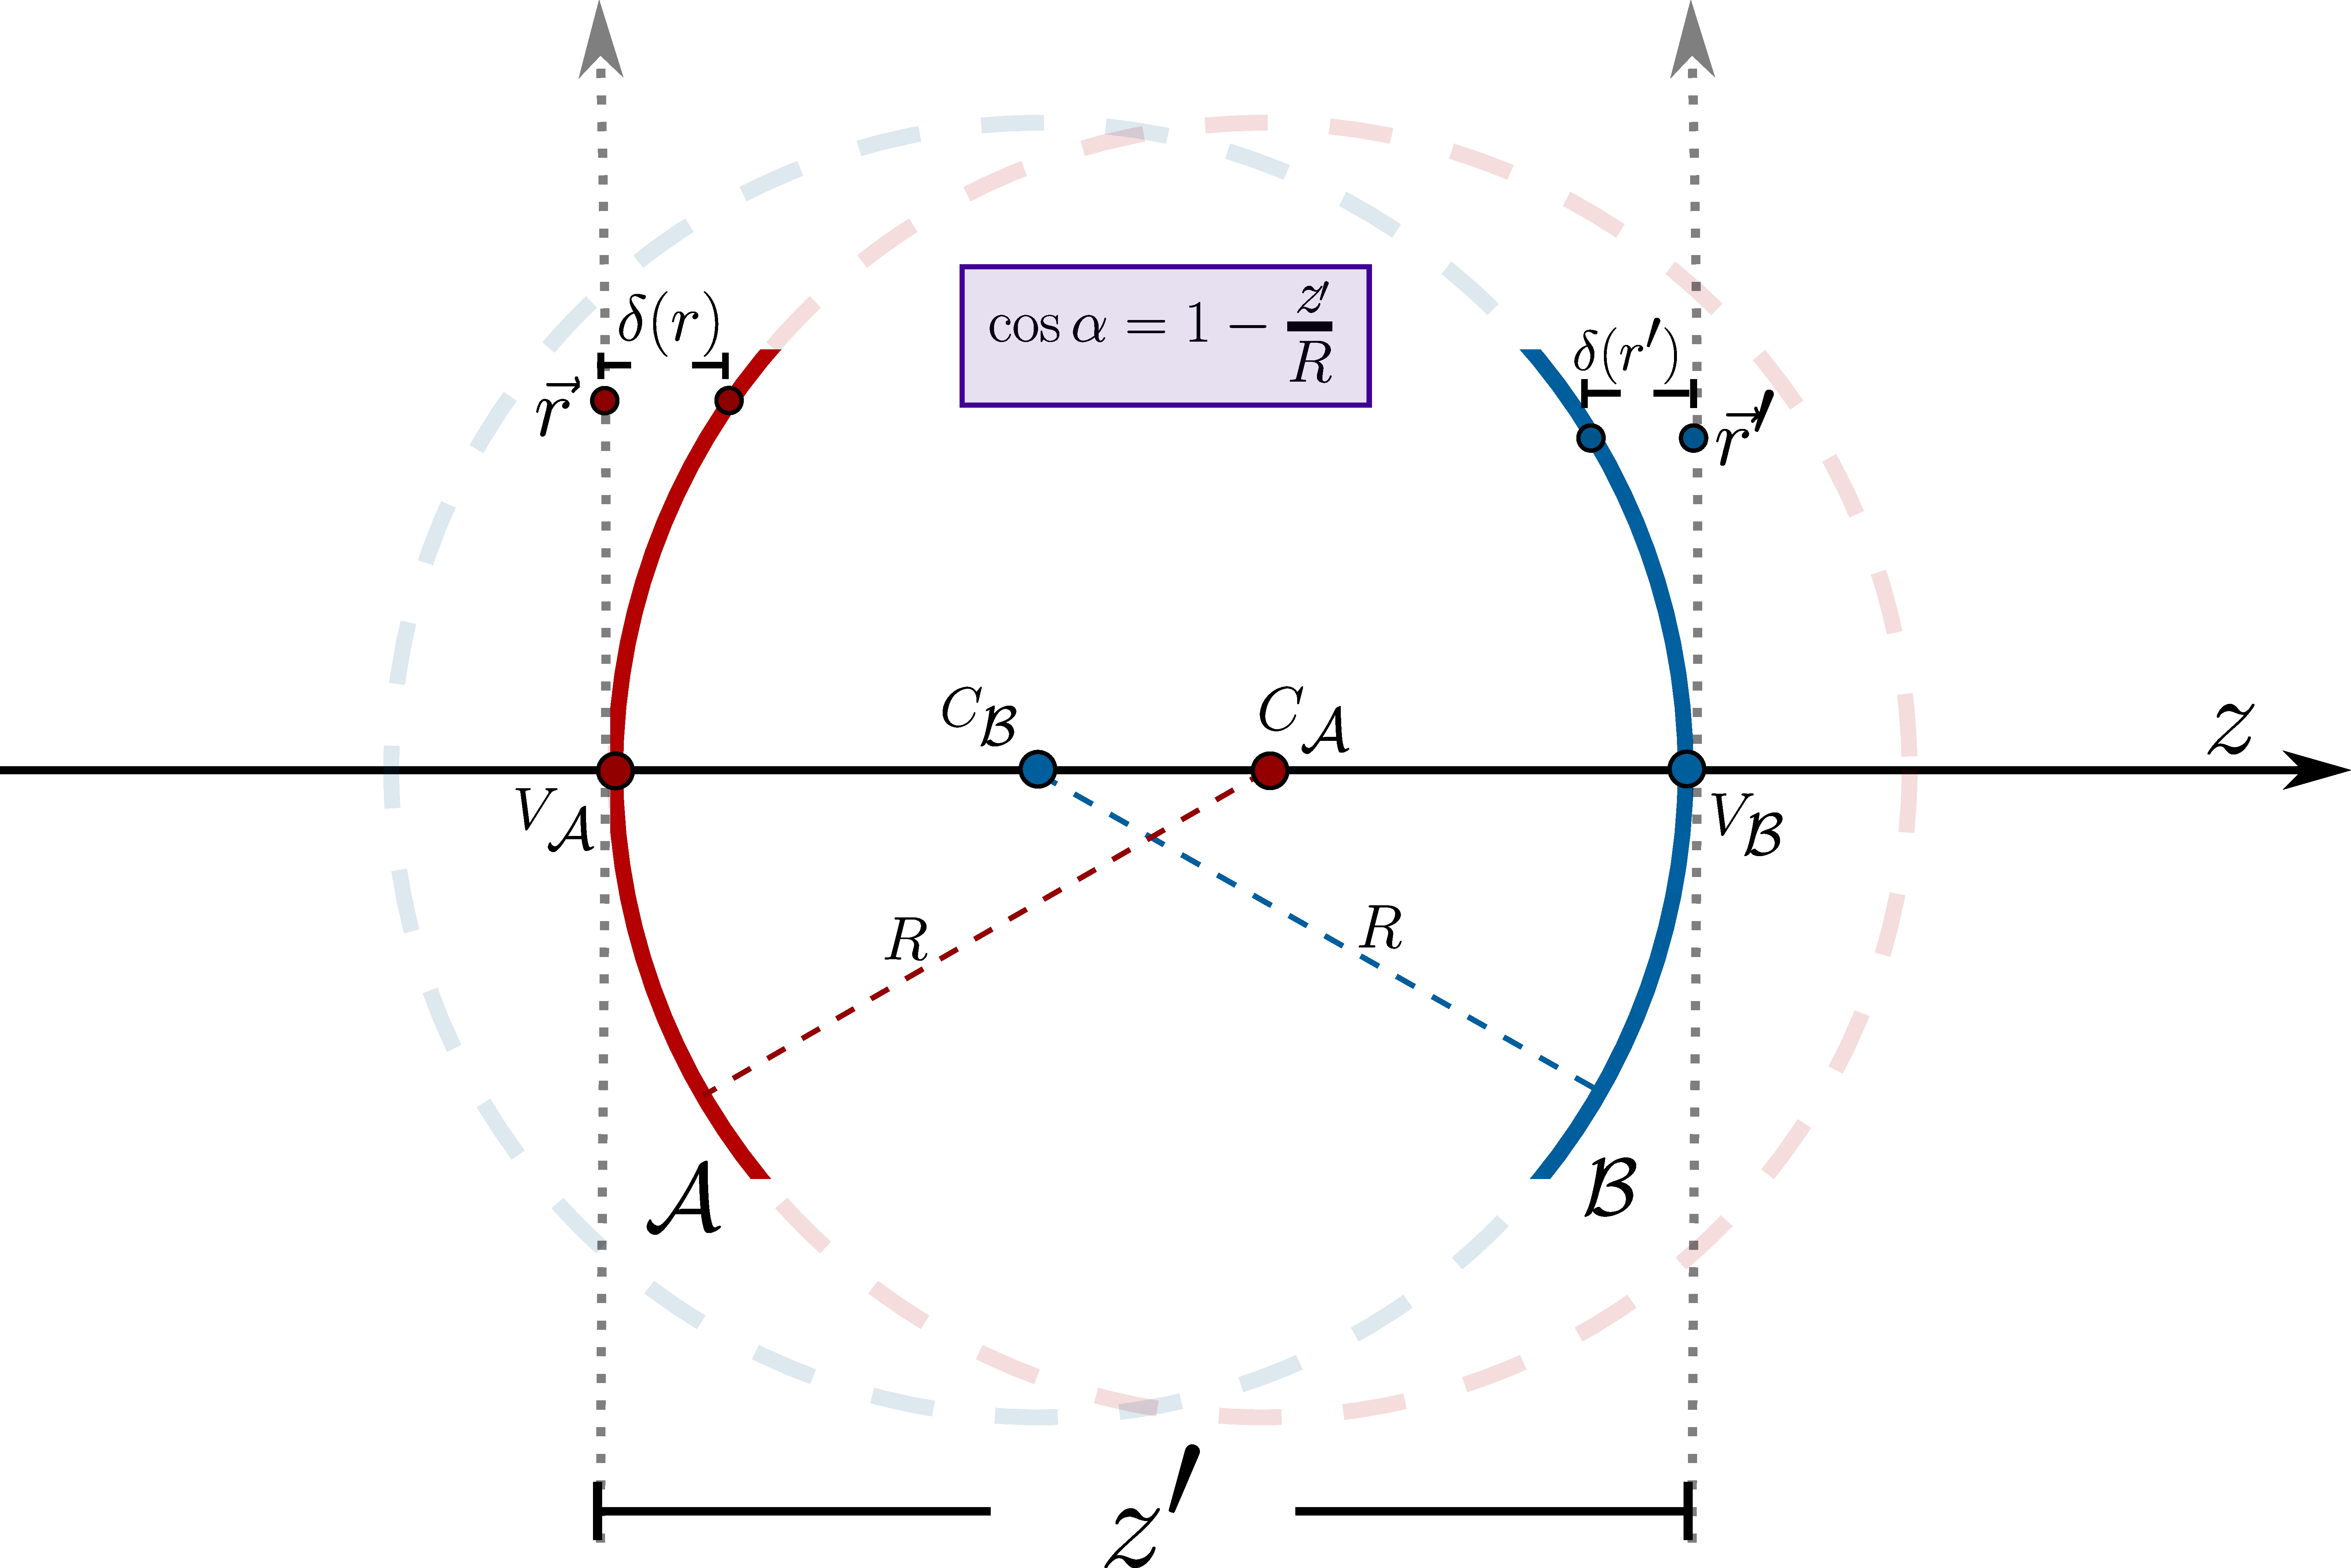
\includegraphics[width=0.8\textwidth]{Capitulo 1/Figuras/CardinalSpheres.pdf}
				\caption{Las dos esferas cardinales de radio $R$ asociadas a una propagación sobre
				la distancia $z$. El casquete emisor $\mathcal{A}$ es tangente a su plano en
				$V_{\mathcal{A}}$ con su centro de curvatura aguas abajo en $C_{\mathcal{A}}$, de
				abscisa $R$, y el casquete receptor $\mathcal{B}$ es tangente a su plano en
				$V_{\mathcal{B}}$ con su centro aguas arriba en $C_{\mathcal{B}}$, de abscisa
				$z-R$, de modo que los dos casquetes se curvan uno hacia el otro. La cantidad $\delta$ es la
				sagita \eqref{eq:FrFT:Sagitta}. El caso confocal de la
				Figura~\ref{fig:ConfocalSpheres} se recupera cuando $R = z$, ya que entonces
				$C_{\mathcal{A}}$ cae sobre $V_{\mathcal{B}}$ y $C_{\mathcal{B}}$ sobre
				$V_{\mathcal{A}}$.}
				\label{fig:CardinalSpheres}
			\end{figure}

			Con \eqref{eq:FrFT:Cardinals} los dos coeficientes cuadráticos colapsan en la única cantidad
			\begin{equation}\label{eq:FrFT:Q}
				Q = \frac{k}{2}\left(\frac{1}{z}-\frac{1}{R}\right),
			\end{equation}
			y la propagación se lee
			\begin{equation}\label{eq:FrFT:SphereToSphere}
				u_{\mathcal{B}}(\vec{r}\,') = \frac{e^{ikz}}{i\lambda z}\int_{\mathbb{R}^{2}} u_{\mathcal{A}}(\vec{r})\exp\left[iQ\left(r^{2}+r'^{2}\right)\right]\exp\left[-\frac{ik}{z}\,\vec{r}\cdot\vec{r}\,'\right]\mathrm{d}^{2}r,
			\end{equation}
			que ahora tiene exactamente la estructura de \eqref{eq:FrFT:Kernel2D} con coeficientes cuadrático y cruzado independientes. Repitiendo la identificación de la subsubsección anterior con las variables reducidas \eqref{eq:FrFT:Reduced},
			\begin{align}
				& Q\,\omega^{2} = \frac{\cot\alpha}{2} \quad\Longrightarrow\quad \cot\alpha = k\,\omega^{2}\left(\frac{1}{z}-\frac{1}{R}\right),\label{eq:FrFT:MatchQuad}\\
				& \frac{k}{z}\,\omega^{2} = \csc\alpha,\label{eq:FrFT:MatchCross}
			\end{align}
			y dividiendo \eqref{eq:FrFT:MatchQuad} entre \eqref{eq:FrFT:MatchCross} la escala $\omega$ se cancela una vez más,
			\begin{equation*}
				\cos\alpha = \frac{\cot\alpha}{\csc\alpha} = \frac{{\color{red}k\,\omega^{2}}\left(\dfrac{1}{z}-\dfrac{1}{R}\right)}{{\color{red}k\,\omega^{2}}\,\dfrac{1}{z}} = z\left(\frac{1}{z}-\frac{1}{R}\right),
			\end{equation*}
			de modo que obtenemos el resultado central
			\begin{equation}\label{eq:FrFT:Order}
				\boxed{\;\cos\alpha = 1 - \frac{z}{R}.\;}
			\end{equation}

			Esta vez no hay contradicción, porque el radio $R$ de los casquetes de referencia está a nuestra disposición. La longitud de escala se sigue de \eqref{eq:FrFT:MatchCross},
			\begin{equation}\label{eq:FrFT:Scale}
				\omega^{2} = \frac{z}{k\sin\alpha} = \frac{\lambda z}{2\pi\sin\alpha},
			\end{equation}
			y, eliminando $\alpha$ mediante \eqref{eq:FrFT:Order} y $\sin^{2}\alpha = 1-\cos^{2}\alpha$,
			\begin{equation*}
				\sin^{2}\alpha = {\color{red}1} - \left({\color{red}1} - \frac{2z}{R} + \frac{z^{2}}{R^{2}}\right) = \frac{z\left(2R-z\right)}{R^{2}} \quad\Longrightarrow\quad \sin\alpha = \frac{\sqrt{z\left(2R-z\right)}}{R},
			\end{equation*}
			cancelándose las dos unidades en rojo, de modo que la longitud de escala se expresa enteramente en términos de la geometría,
			\begin{equation}\label{eq:FrFT:ScaleExplicit}
				\omega^{2} = \frac{\lambda R}{2\pi}\sqrt{\frac{z}{2R-z}}.
			\end{equation}

		\subsubsection{La constante de normalización y el resultado final}

			Resta comparar las constantes. Cambiando variables en \eqref{eq:FrFT:SphereToSphere} según \eqref{eq:FrFT:Reduced}, de modo que $\mathrm{d}^{2}r = \omega^{2}\,\mathrm{d}^{2}u$,
			\begin{equation}\label{eq:FrFT:Reduced2}
				u_{\mathcal{B}}(\omega\vec{v}) = \frac{e^{ikz}\,\omega^{2}}{i\lambda z}\int_{\mathbb{R}^{2}} u_{\mathcal{A}}(\omega\vec{u})\exp\left[\frac{i}{2}\left(u^{2}+v^{2}\right)\cot\alpha - i\,\vec{u}\cdot\vec{v}\csc\alpha\right]\mathrm{d}^{2}u,
			\end{equation}
			y usando \eqref{eq:FrFT:Scale} el prefactor se simplifica a
			\begin{equation}\label{eq:FrFT:PrefactorOptics}
				\frac{\omega^{2}}{i\lambda z} = \frac{1}{i\,{\color{red}\lambda z}}\cdot\frac{{\color{red}\lambda z}}{2\pi\sin\alpha} = \frac{1}{2\pi i\sin\alpha} = \frac{-i}{2\pi\sin\alpha}.
			\end{equation}
			Por otra parte la constante de \eqref{eq:FrFT:Kernel2D}, reescrita mediante la identidad \eqref{eq:FrFT:ConstantEquiv}, es
			\begin{equation}\label{eq:FrFT:PrefactorFrFT}
				\frac{1-i\cot\alpha}{2\pi} = \frac{1}{2\pi}\cdot\frac{e^{-i\pi/2}e^{i\alpha}}{\sin\alpha} = \frac{-i\,e^{i\alpha}}{2\pi\sin\alpha}.
			\end{equation}
			Dividiendo \eqref{eq:FrFT:PrefactorOptics} entre \eqref{eq:FrFT:PrefactorFrFT},
			\begin{equation*}
				\frac{\;\dfrac{-i}{{\color{red}2\pi\sin\alpha}}\;}{\dfrac{-i\,e^{i\alpha}}{{\color{red}2\pi\sin\alpha}}} = \frac{-i}{-i}\,e^{-i\alpha} = e^{-i\alpha},
			\end{equation*}
			y por lo tanto, reuniendo todo, hemos demostrado el teorema.

			\begin{myteo}
				\textit{(La difracción de Fresnel como transformación fraccionaria de Fourier)} Sea el campo referido a dos casquetes esféricos cardinales de radio $R$ separados por la distancia $z$ a lo largo del eje, en el sentido de \eqref{eq:FrFT:Cardinals}, y sean las coordenadas transversales reducidas por la escala $\omega$ de \eqref{eq:FrFT:ScaleExplicit}. Entonces la propagación de Fresnel \eqref{Fresnel} es la transformación fraccionaria de Fourier
				\begin{equation}\label{eq:FrFT:MainResult}
					u_{\mathcal{B}}(\omega\vec{v}) = e^{i\left(kz - \alpha\right)}\left(\mathcal{F}_{\alpha}\,u_{\mathcal{A}}\right)(\vec{v}),
				\end{equation}
				cuyo orden está dado por $\cos\alpha = 1 - z/R$.
			\end{myteo}

			Es pertinente un comentario sobre la fase residual. Aparte del factor trivial $e^{ikz}$, que simplemente cuenta el camino óptico a lo largo del eje, la propagación deja atrás el factor $e^{-i\alpha}$ y nada más. Esto es una consecuencia directa de la normalización $1/(i\lambda z)$ de la integral de Fresnel \eqref{Fresnel}, aquella para la cual el núcleo tiende a $\delta(\vec{r}-\vec{r}\,')$ cuando $z\to0$; si la constante se hubiera escrito con el signo opuesto, habría aparecido un $\pi$ aditivo en el exponente de \eqref{eq:FrFT:MainResult} sin contenido físico alguno. Con la normalización correcta, el orden $\alpha$ es exactamente la fase de Gouy acumulada, punto al que volveremos.

			Probemos \eqref{eq:FrFT:MainResult} en los tres casos que podemos verificar de manera independiente.

			\begin{enumerate}
				\item \textbf{$z = 0$.} La ecuación \eqref{eq:FrFT:Order} da $\cos\alpha = 1$, de donde $\alpha = 0$ y $\mathcal{F}_{0} = \mathcal{I}$: el campo sobre el casquete receptor es el campo sobre el casquete emisor, como debe ser.
				\item \textbf{$z = R$.} Ahora $\cos\alpha = 0$, de donde $\alpha = \pi/2$ y la transformación es la transformación de Fourier ordinaria. Esto no es una coincidencia: cuando $z=R$ el casquete emisor tiene su centro en la abscisa $R = z$, que es el vértice del casquete receptor, y el casquete receptor tiene su centro en $z-R = 0$, que es el vértice del casquete emisor. Los dos casquetes son por lo tanto \textit{las esferas cardinales confocales} de la Figura~\ref{fig:cardinals}, y recuperamos exactamente el resultado de Fraunhofer \eqref{Fraunhofer} de la sección anterior. La descripción de campo lejano es el caso particular $\alpha = \pi/2$ de la presente.
				\item \textbf{$z = 2R$.} Aquí $\cos\alpha = -1$, de donde $\alpha = \pi$ y $\mathcal{F}_{\pi} = \mathcal{P}$: el campo sobre el casquete receptor es el campo sobre el casquete emisor invertido. Dos transformaciones de Fourier consecutivas invierten la imagen, y la geometría dice lo mismo.
			\end{enumerate}

			La ganancia en economía es considerable. En la descripción plano a plano, encadenar dos propagaciones de distancias $z_{1}$ y $z_{2}$ exige componer dos integrales de Fresnel, y el núcleo compuesto debe recalcularse cada vez. En la presente descripción la composición es la ley de índices \eqref{eq:FrFT:IndexLaw},
			\begin{equation}\label{eq:FrFT:Chaining}
				\mathcal{F}_{\alpha_{2}}\mathcal{F}_{\alpha_{1}} = \mathcal{F}_{\alpha_{1}+\alpha_{2}},
			\end{equation}
			de modo que la propagación se describe mediante la adición de ángulos. Las distancias $z$ no se suman de ninguna manera útil, pero los órdenes sí, y este es el sentido preciso en el cual $\alpha$, y no $z$, es el parámetro natural de la propagación paraxial libre.

		\subsubsection{Significado físico de un orden real}

			Cuando $\alpha$ es real, \eqref{eq:FrFT:Order} exige $\left|1-z/R\right|\leq 1$, es decir
			\begin{equation}\label{eq:FrFT:RealRange}
				0 \leq z \leq 2R,
			\end{equation}
			y el orden recorre monótonamente el intervalo $[0,\pi]$ conforme el casquete de observación se aleja. La lectura de $\alpha$ es entonces completamente transparente, y hay tres maneras equivalentes de enunciarla.

			\textit{Como un grado de difracción.} El orden mide cuán lejos ha viajado el campo desde el campo cercano hacia el campo lejano, en una escala en la cual $\alpha = 0$ es la propia abertura y $\alpha = \pi/2$ es su patrón de Fraunhofer. Un campo observado en $\alpha = \pi/4$ está a medio camino entre su propia distribución y su transformada de Fourier, en un sentido que no es metafórico sino exacto, ya que aplicar dos veces la misma transformación produce la transformada de Fourier. El continuo de regímenes intermedios que la aproximación de Fresnel describe solo implícitamente queda aquí etiquetado por un único número.

			\textit{Como una rotación del espacio de fase.} Por el teorema de Lohmann \citeyearpar{lohmann1993image}, establecido después con rigor por Mustard \citeyearpar{mustard1996fractional}, la transformación $\mathcal{F}_{\alpha}$ actúa sobre la distribución de Wigner del campo simplemente rotando el plano de la posición transversal y la frecuencia espacial transversal por el ángulo $\alpha$. La propagación libre entre esferas cardinales es por lo tanto una rotación rígida del espacio de fase, razón por la cual los órdenes se suman: las rotaciones se componen sumando ángulos. Esto también explica geométricamente por qué la propagación plano a plano no es una transformación fraccionaria, ya que en la descripción por planos la propagación es una cizalla del espacio de fase en lugar de una rotación.

			\textit{Como una fase de Gouy.} El factor residual $e^{-i\alpha}$ de \eqref{eq:FrFT:MainResult} no es accidental. Si en lugar de casquetes arbitrarios se eligen como superficies de referencia los frentes de onda de un haz gaussiano de rango de Rayleigh $z_{R}$, el orden que resulta del mismo cálculo es
			\begin{equation}\label{eq:FrFT:Gouy}
				\alpha = \arctan\!\left(\frac{z}{z_{R}}\right),
			\end{equation}
			que es precisamente la fase de Gouy acumulada del haz \citep{ozaktas1995fractional}. La identificación es satisfactoria, ya que \eqref{eq:FrFT:Gouy} tiende a $\pi/2$ cuando $z\to\infty$, recuperando una vez más el enunciado de que el campo lejano es la transformada de Fourier del campo cercano, y muestra que la misteriosa fase adicional de un haz enfocado no es sino el orden de la transformación fraccionaria que el haz ha sufrido.

			Debe subrayarse un punto, porque es una fuente frecuente de confusión. \textit{El orden no es una propiedad de la propagación por sí sola.} Es una propiedad del par formado por la propagación y los dos casquetes de referencia, ya que \eqref{eq:FrFT:Order} involucra tanto a $z$ como a $R$. Dada una distancia de propagación $z$, puede obtenerse cualquier orden que se desee eligiendo
			\begin{equation}\label{eq:FrFT:ChooseR}
				R = \frac{z}{1-\cos\alpha},
			\end{equation}
			y recíprocamente el mismo par de casquetes asigna órdenes distintos a distancias distintas. Lo que es intrínseco no es $\alpha$ sino la estructura de grupo: sean cuales sean los casquetes de referencia elegidos, la propagación está representada por un elemento del mismo grupo uniparamétrico.

		\subsubsection{Significado físico de un orden complejo}

			La condición \eqref{eq:FrFT:RealRange} es una restricción real, y es natural preguntarse qué sucede cuando se viola. Si el radio $R$ de los casquetes se mantiene fijo mientras la distancia de propagación excede $2R$, o si la propagación se hace correr hacia atrás de modo que $z<0$, entonces $\cos\alpha$ abandona el intervalo $[-1,1]$ y el orden se vuelve complejo. Escribiendo $\alpha = \alpha_{r} + i\alpha_{i}$ hay dos casos.

			Para $\cos\alpha > 1$, que corresponde a $z<0$ con $R>0$, el orden es puramente imaginario, $\alpha = i\beta$ con
			\begin{equation}\label{eq:FrFT:ImagOrder}
				\cosh\beta = 1 - \frac{z}{R}.
			\end{equation}

			Para $\cos\alpha < -1$, que corresponde a $z>2R$, el orden es $\alpha = \pi + i\beta$ con $\cosh\beta = z/R - 1$, cargando el $\pi$ aditivo la inversión de la imagen que ya encontramos en $z=2R$.

			La consecuencia sobre el núcleo es inmediata y físicamente elocuente. Tomando el primer caso y usando $\cot(i\beta) = -i\coth\beta$ y $\csc(i\beta) = -i\operatorname{csch}\beta$, el exponente de \eqref{eq:FrFT:Kernel2D} se convierte en
			\begin{align*}
				& \frac{i}{2}\left(u^{2}+v^{2}\right)\left(-i\coth\beta\right) - i\,\vec{u}\cdot\vec{v}\left(-i\operatorname{csch}\beta\right) = \\
				& \frac{1}{2}\left(u^{2}+v^{2}\right)\coth\beta - \vec{u}\cdot\vec{v}\operatorname{csch}\beta,
			\end{align*}
			que es \textit{enteramente real}. El núcleo ha dejado de ser un chirp puro y se ha convertido en una gaussiana real, y puesto que
			\begin{equation*}
				\coth\beta - \operatorname{csch}\beta = \frac{\cosh\beta - 1}{\sinh\beta} > 0 \qquad (\beta>0),
			\end{equation*}
			la forma cuadrática asociada es definida positiva, de modo que el núcleo crece en lugar de oscilar. Esta es la firma analítica de un problema mal planteado, y es exactamente lo que cabría esperar, ya que $z<0$ es retropropagación y la retropropagación amplifica sin límite el contenido de alta frecuencia espacial del campo. El orden complejo no se limita a describir la dificultad, la cuantifica: la parte imaginaria $\beta$ es el exponente de la amplificación gaussiana.

			De manera más general, un orden complejo admite tres lecturas físicas complementarias.

			\begin{enumerate}
				\item \textbf{Desde la teoría de grupos}, un orden real corresponde a un elemento elíptico del grupo de transformaciones canónicas lineales, es decir, a una rotación del espacio de fase, mientras que un orden complejo corresponde a un elemento que también contiene una compresión (\textit{squeeze}), es decir, una magnificación a lo largo de una dirección del espacio de fase y una compresión a lo largo de la otra. Un orden complejo anuncia por lo tanto que la transformación es una rotación compuesta con un escalamiento, y la parte imaginaria mide ese escalamiento.
				\item \textbf{Para haces gaussianos}, la curvatura del frente de onda no es un número real sino el parámetro complejo $q$ definido por $q^{-1} = R^{-1} - i\lambda/(\pi w^{2})$, donde $w$ es el radio del haz. Sustituyendo $q$ por $R$ en \eqref{eq:FrFT:Order} se obtiene automáticamente un orden complejo, cuya parte real es la rotación del espacio de fase y cuya parte imaginaria lleva la envolvente gaussiana del haz. Las transformaciones fraccionarias de orden complejo son, por esta razón, el lenguaje natural de la propagación de haces gaussianos, y fueron realizadas ópticamente por Shih \citeyearpar{shih1995optical} y por Bernardo y Soares \citeyearpar{bernardo1996optical}.
				\item \textbf{Para sistemas apodizados}, una abertura gaussiana $e^{-r^{2}/a^{2}}$ colocada en el haz contribuye exactamente con un factor gaussiano real del tipo que produce un orden complejo. La parte imaginaria del orden mide entonces la atenuación del contenido de $|\vec{u}|$ grande del campo, es decir, un filtrado pasa-bajas gaussiano en el dominio fraccionario, que en la imagen es una pérdida de resolución. Un orden complejo es, en esta lectura, el mecanismo de contabilidad para aberturas suaves y para pérdidas.
			\end{enumerate}

			Por último, debe subrayarse que un orden complejo nunca señala una imposibilidad física. Puesto que \eqref{eq:FrFT:ChooseR} muestra que el orden depende de los casquetes de referencia, cualquier propagación hacia adelante con $z>0$ puede describirse con un orden real simplemente eligiendo $R \geq z/2$. Lo que un orden complejo señala es que las superficies de referencia elegidas no son aquellas respecto a las cuales la propagación es una rotación pura. El caso límite de esta afirmación es el plano, para el cual $R\to\infty$ da $\cos\alpha\to1$ y, por \eqref{eq:FrFT:Scale}, $\omega\to\infty$: la transformación degenera, el ángulo de rotación colapsa a cero mientras la escala diverge, y recuperamos el teorema de la primera subsubsección de que la propagación de Fresnel plano a plano queda fuera de la familia fraccionaria de Fourier. Todo el contenido del resultado de Pellat-Finet es que la familia se recupera tan pronto se acepta mirar el campo sobre una esfera.
